
\begingroup
% move all floats to the end of the chapter
\renewcommand{\textfraction}{1.0}
\renewcommand{\floatpagefraction}{0.9}

\chapter{Results}
\label{ch:results}

The three implementations discussed in \cref{ch:direct_intersection,ch:tri_dexel,ch:point_cloud_based} have been tested on the scenes described in chapter \cref{ch:test_scenes}.
Each implementation has been benchmarked on the same machine, utilizing an Intel Core i7-3770 quad-core processor at \SI{3.4}{\giga\hertz} with \SI{16}{\gibi\byte} RAM.
All timings in this chapter are averaged over ten runs, unless stated otherwise.
The CPU utilization of each algorithm is shown as well, measured using the profiler of Microsoft Visual Studio 2013.
The meshes reconstructed by each implementation at every scene have been rendered using MeshLab \cite{meshlab}.
Where appropriate, detailed renderings are shown to discuss special aspects of an implementation.
Finally, the number of created boundary edges is given for each reconstructed mesh as measured by MeshLab.


\section{Direct intersection}
\label{sec:direct_intersection_results}

The runtime and output size of the test runs of the direct intersection surface reconstruction, \cf \cref{ch:direct_intersection}, are detailed in \cref{tbl:direct_intersection_results}.

\begin{table}
	\centering
	\begin{tabular}{lrrrrr}
		scene         &  SVs &                 t\sub{in} &               t\sub{out} &                               {time} &  \\
		\midrule
		\cubes        &    1 & \SI{  0.8}{\kilo\nothing} & \SI{   1}{\kilo\nothing} &            \SI{  1.0}{\milli\second} &  \\
		\cylindersd   &    1 & \SI{    7}{\kilo\nothing} & \SI{  10}{\kilo\nothing} &            \SI{  6.0}{\milli\second} &  \\
		\cylinders    &    1 & \SI{    4}{\kilo\nothing} & \SI{   7}{\kilo\nothing} &            \SI{  9.0}{\milli\second} &  \\
		\cylinderhead &   20 & \SI{   80}{\kilo\nothing} & \SI{ 149}{\kilo\nothing} &            \SI{229.0}{\milli\second} &  \\
		\impeller     & 2383 & \SI{ 6000}{\kilo\nothing} & \SI{1677}{\kilo\nothing} & \SI{ 21.0}{      \second}\phantom{m} &  \\
		\impellerhalf & 1191 & \SI{ 3000}{\kilo\nothing} & \SI{1296}{\kilo\nothing} & \SI{ 11.0}{      \second}\phantom{m} &  \\
		\turbine      &  480 & \SI{16000}{\kilo\nothing} & \SI{ 752}{\kilo\nothing} & \SI{280.0}{      \second}\phantom{m} &
	\end{tabular}
	\caption[Direct intersection results]{
		Test results for the direct intersection surface extraction approach.
	}
	\label{tbl:direct_intersection_results}
\end{table}

The CPU utilization during an single run of the direct intersection approach on the \impeller scene is shown in \cref{fig:di_cpu}.

\begin{figure}
	\centering
	\begin{tikzpicture}
	\begin{axis}[
		width=0.95\textwidth,
		height=0.5\textwidth,
		xlabel={Wall clock time in \si{\second}},
		ylabel={CPU utilization in \si{\percent}},
		ymin=0,
		ymax=100,
		ytick={0,20,...,100},
		%xtick={0,3,...,99}
	]
	\addplot table [x=time, y=utilization, col sep=comma]{spreadsheets/di_hq_impeller_cpu.csv};
	\end{axis}
	\end{tikzpicture}
	%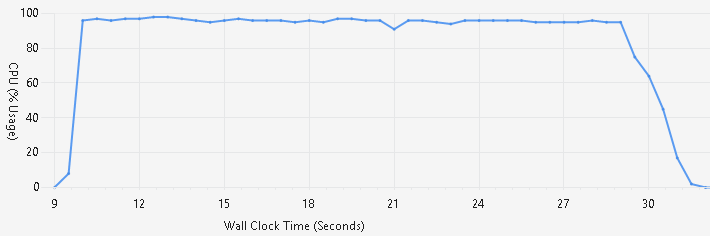
\includegraphics[width=0.8\textwidth]{di_hq_impeller_cpu}
	\caption[Direct intersection CPU utilization]{
		CPU utilization during a run of the direct intersection algorithm to reconstruct the surface of the \impeller scene.
	}
	\label{fig:di_cpu}
\end{figure}

\Cref{fig:di_results} contains renderings of the resulting triangle meshes.

\begin{figure}
	\centering
	\begin{subfigure}[b]{0.34\textwidth}
		\centering
		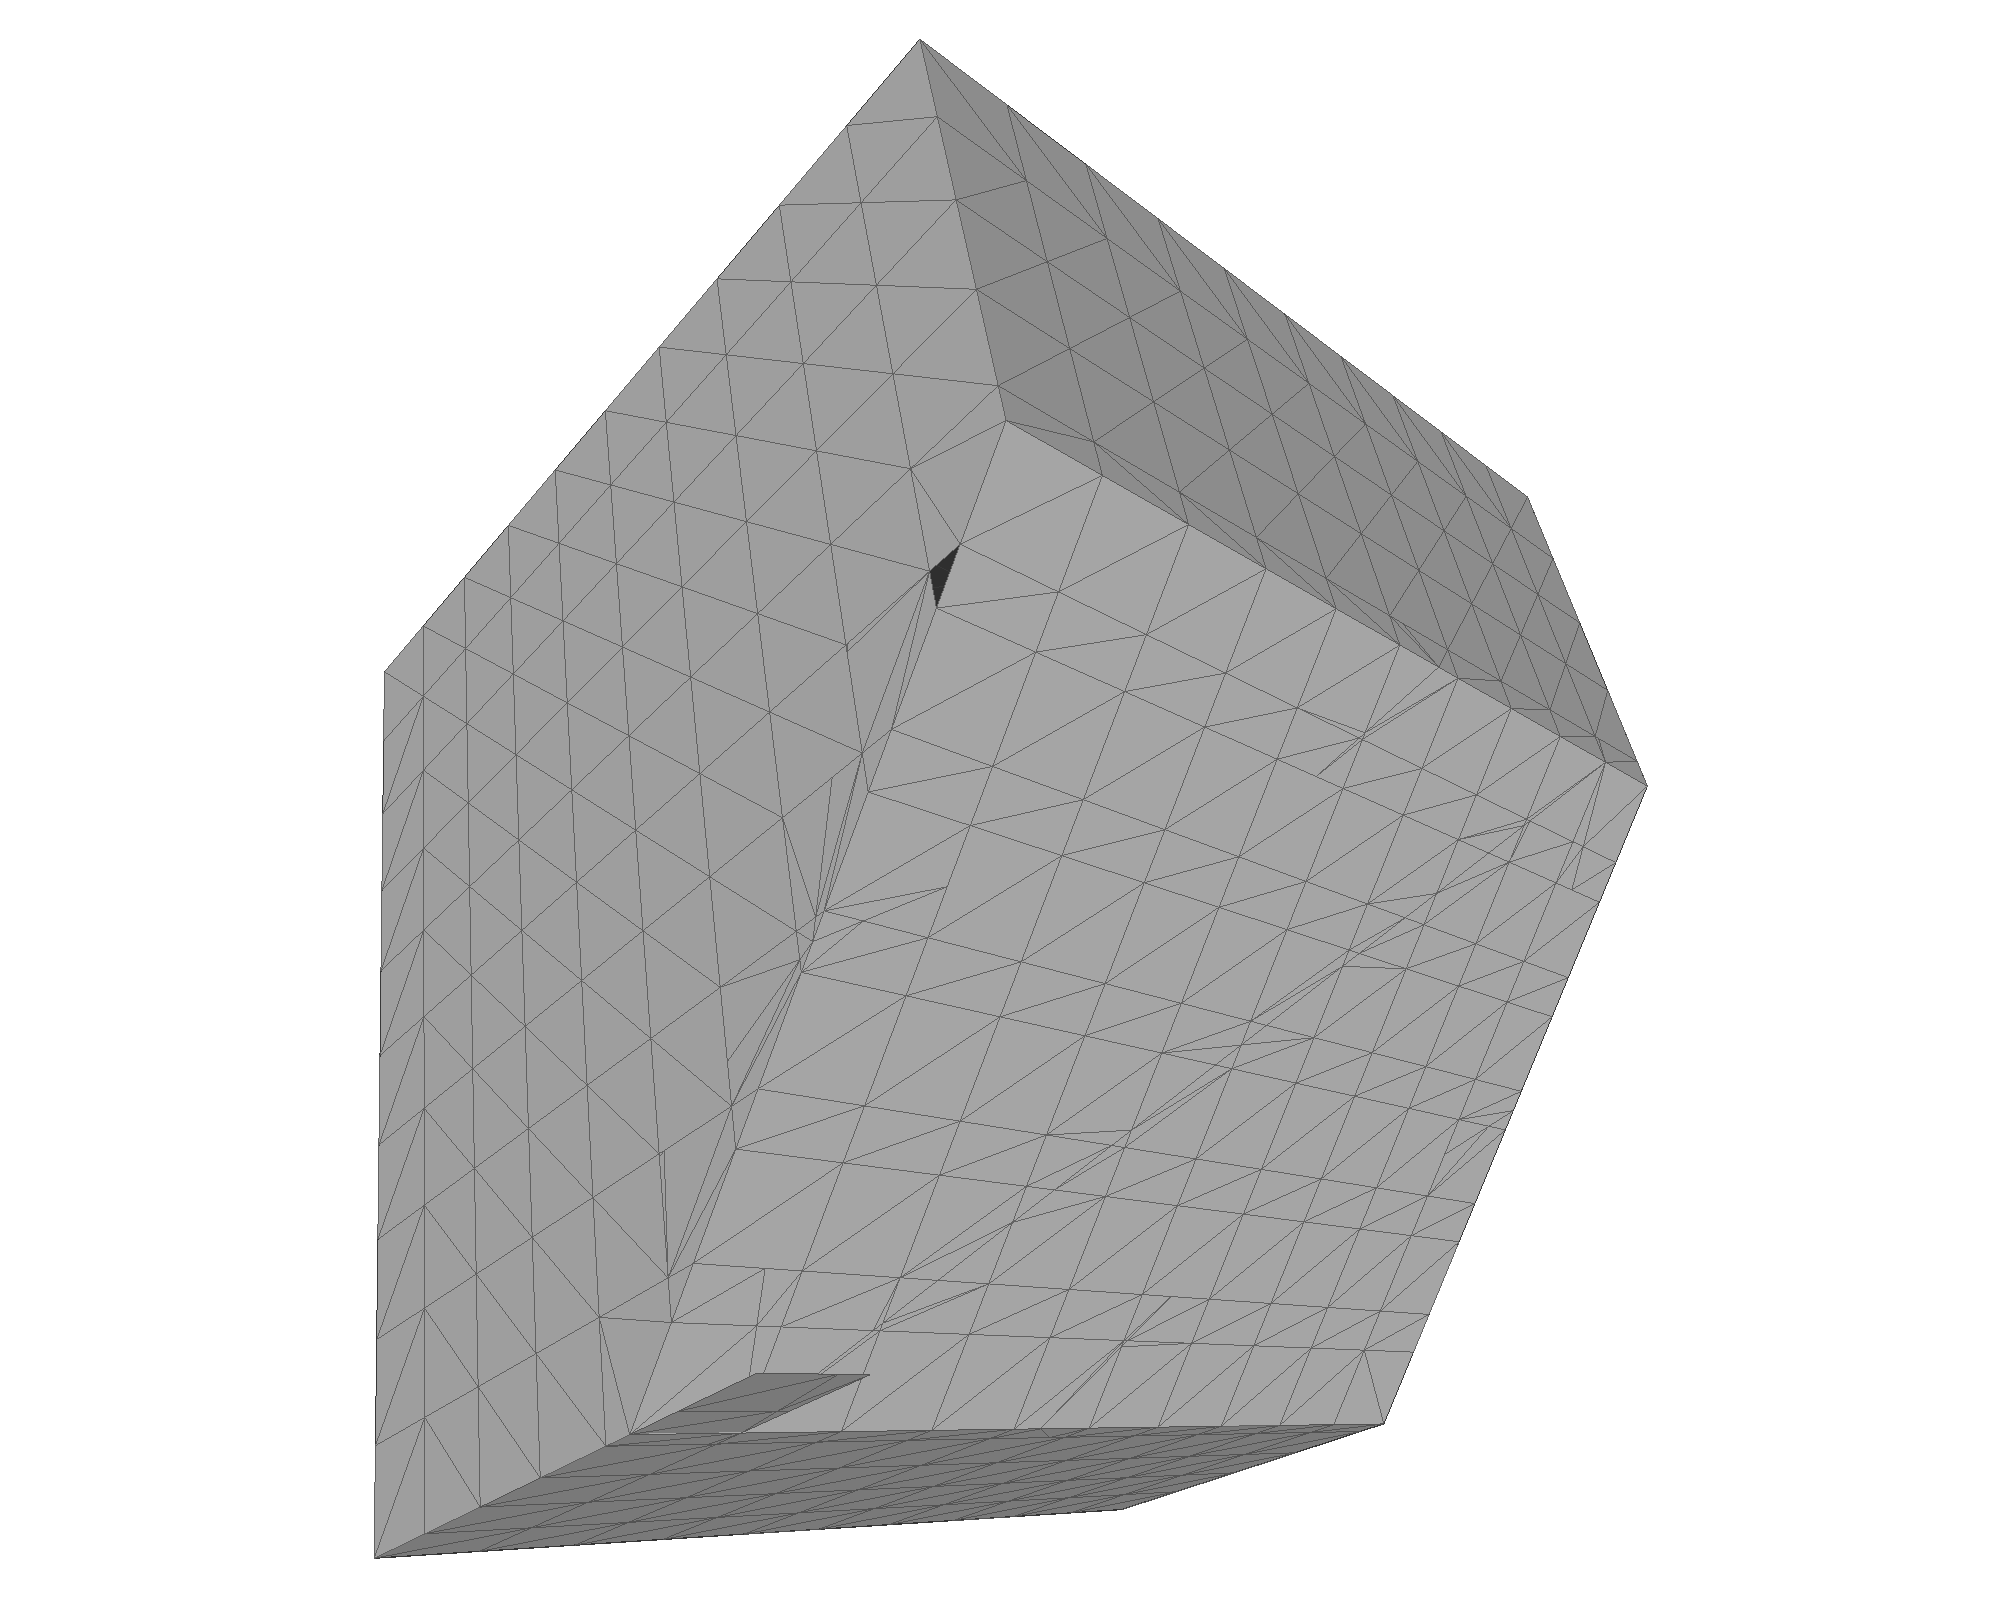
\includegraphics[width=\textwidth]{di_cube2}
		\caption{\cubes}
		\label{fig:di_cube2}
	\end{subfigure}
	\hspace{1cm}
	\begin{subfigure}[b]{0.34\textwidth}
		\centering
		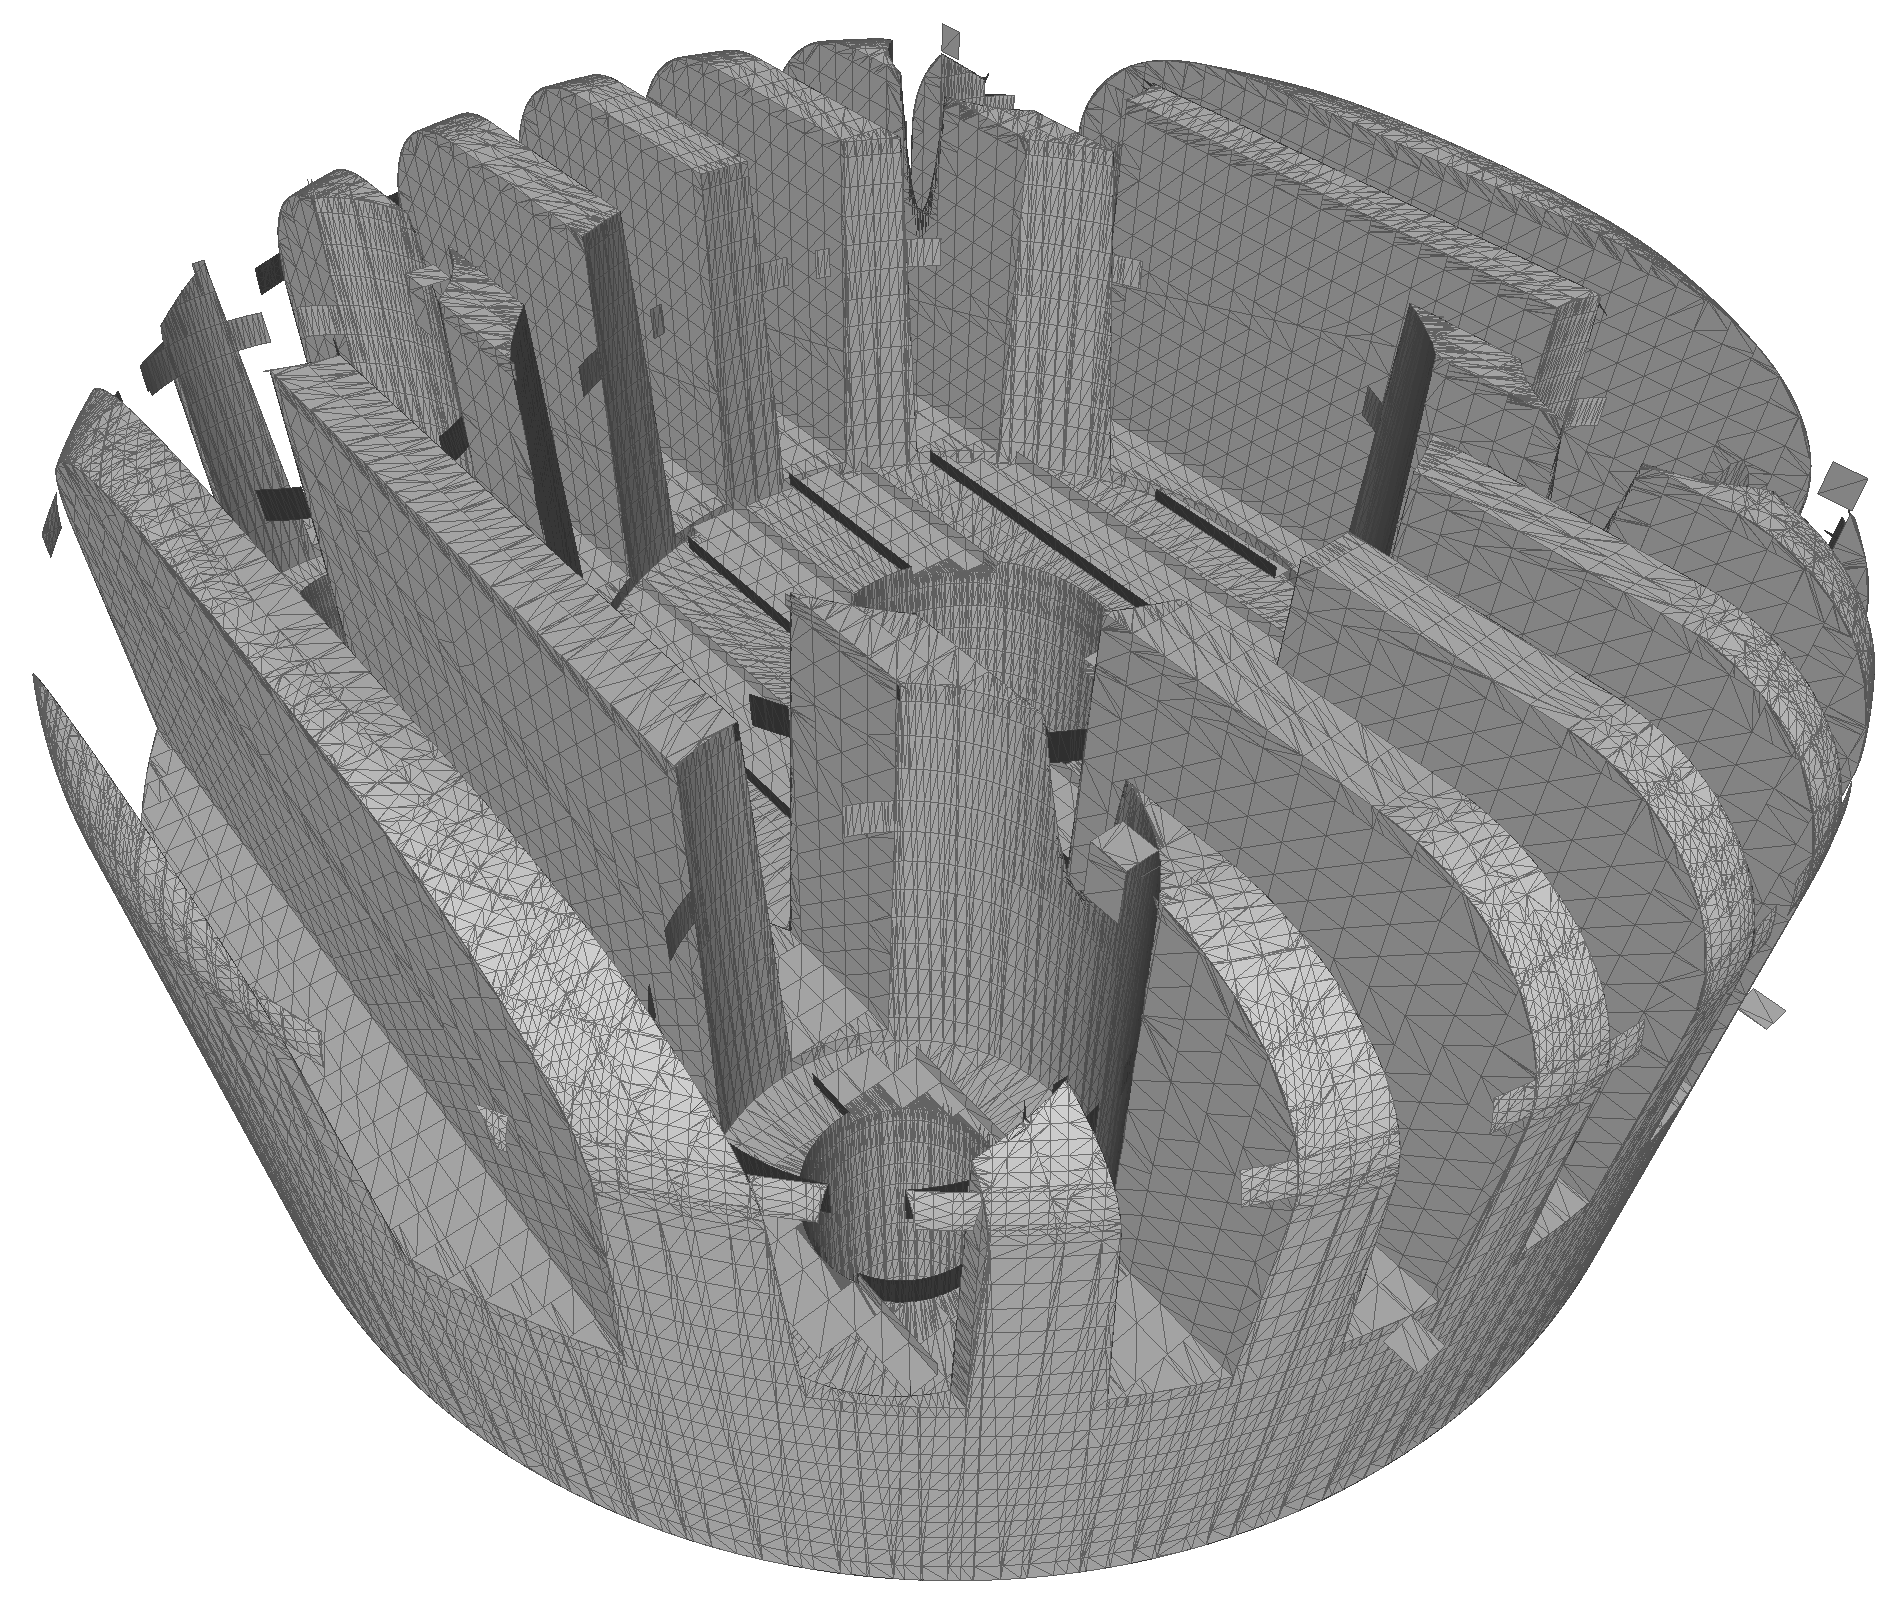
\includegraphics[width=\textwidth]{di_cylinder_head}
		\caption{\cylinderhead}
		\label{fig:di_cylinder_head}
	\end{subfigure}
	\begin{subfigure}[b]{0.34\textwidth}
		\centering
		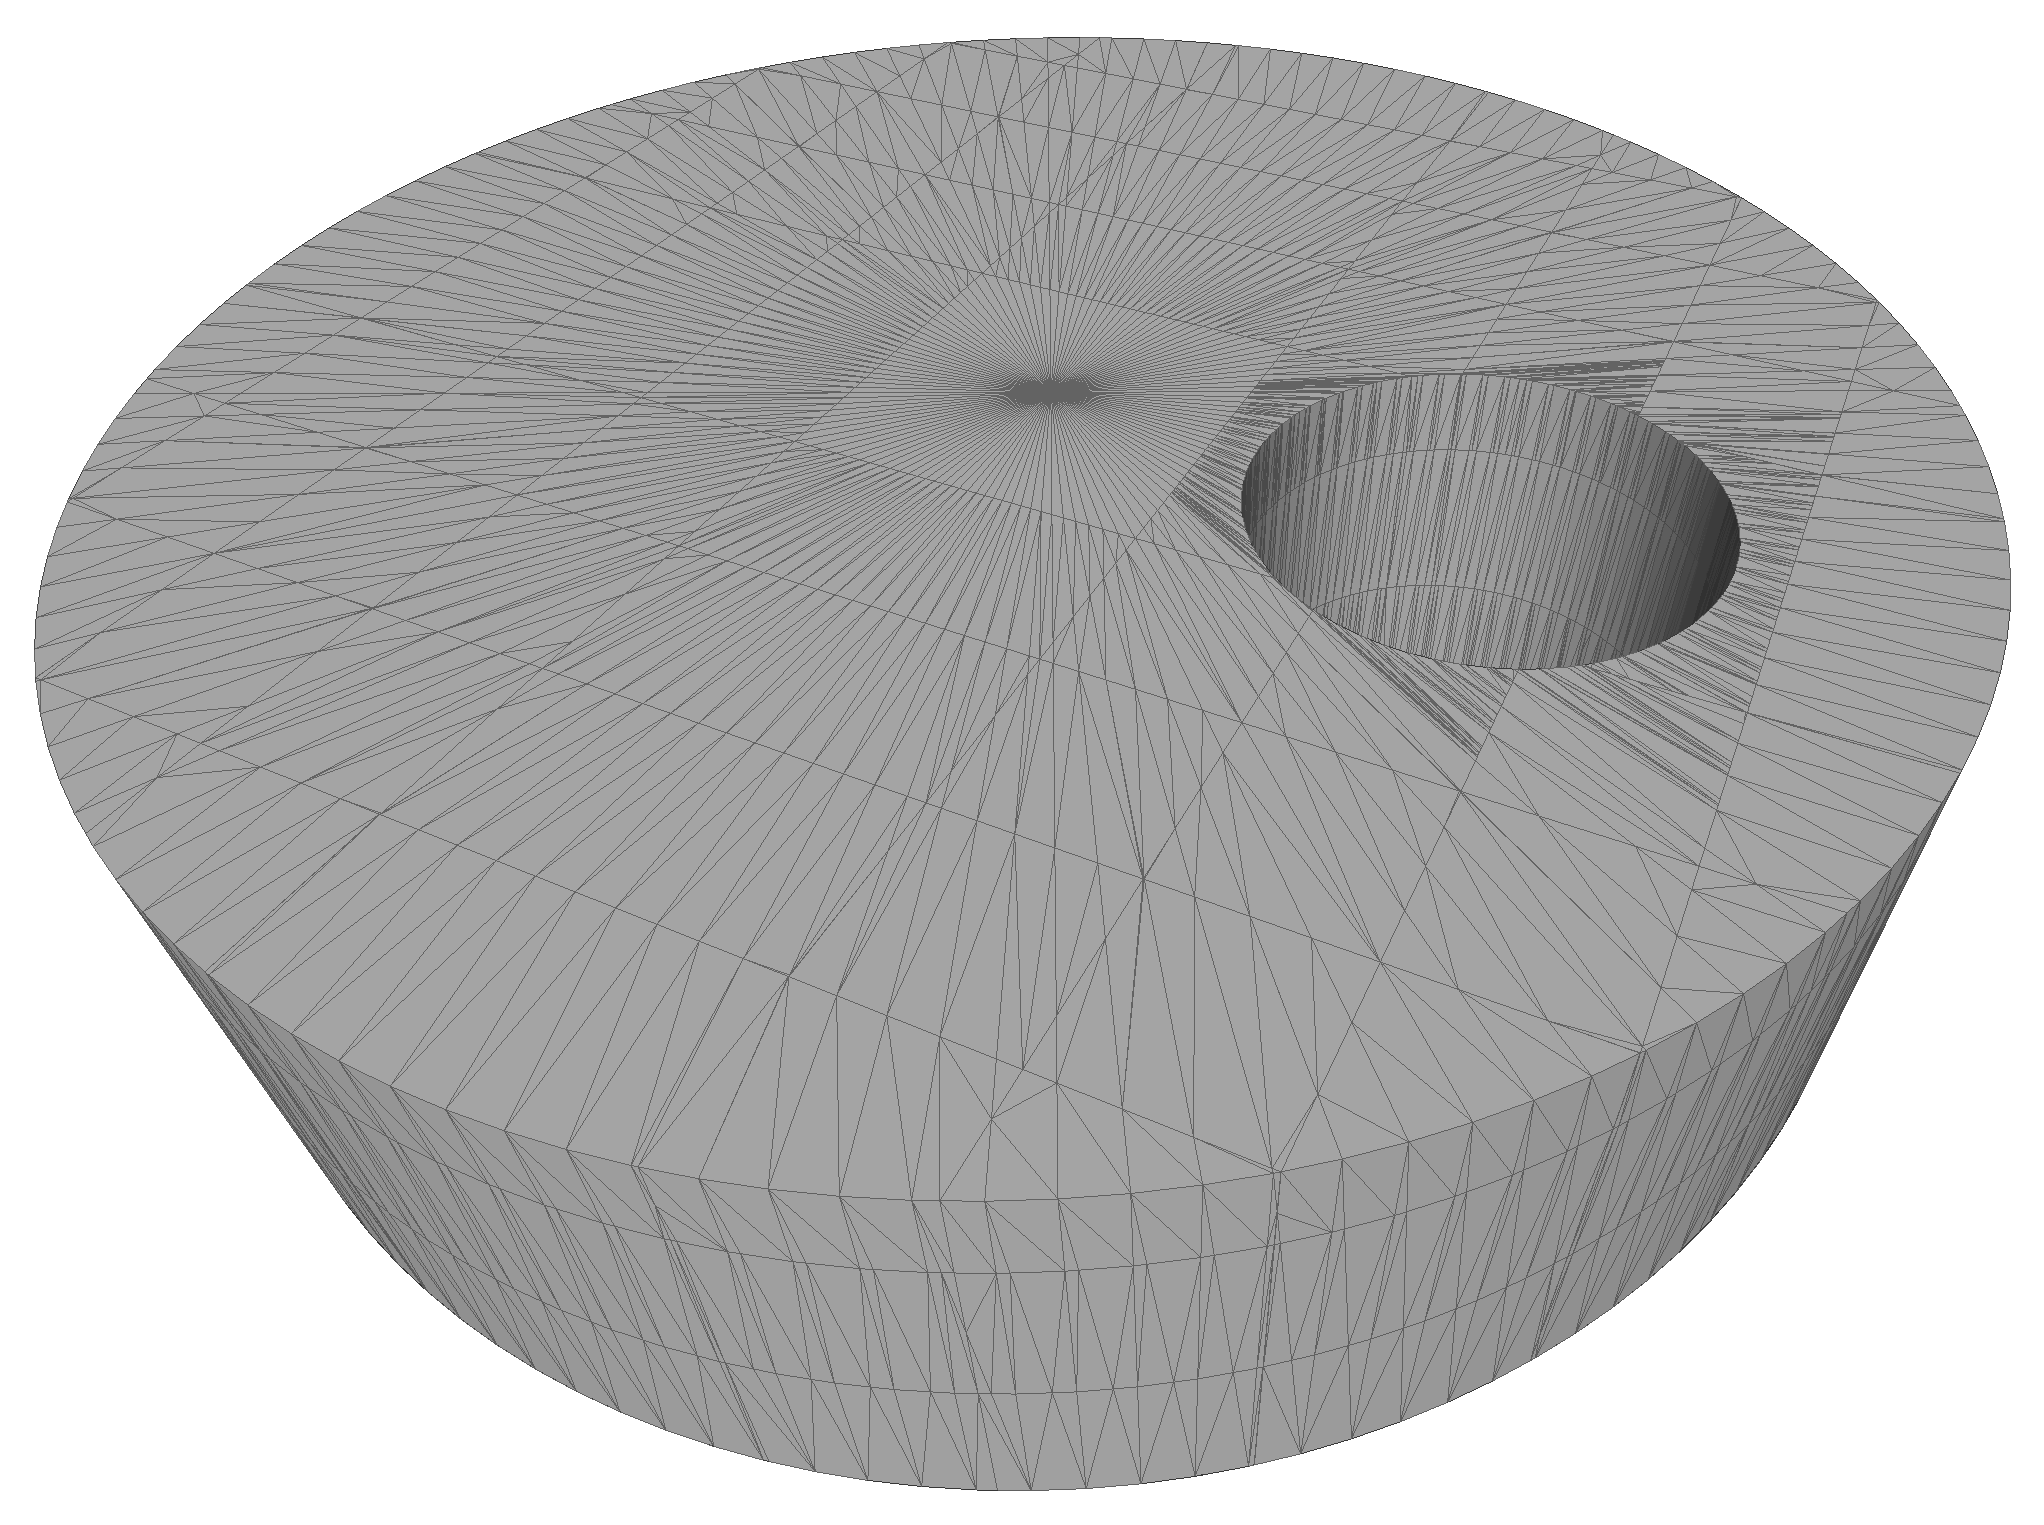
\includegraphics[width=\textwidth]{di_cylinders}
		\caption{\cylinders}
		\label{fig:di_cylinders}
	\end{subfigure}
	\hspace{1cm}
	\begin{subfigure}[b]{0.34\textwidth}
		\centering
		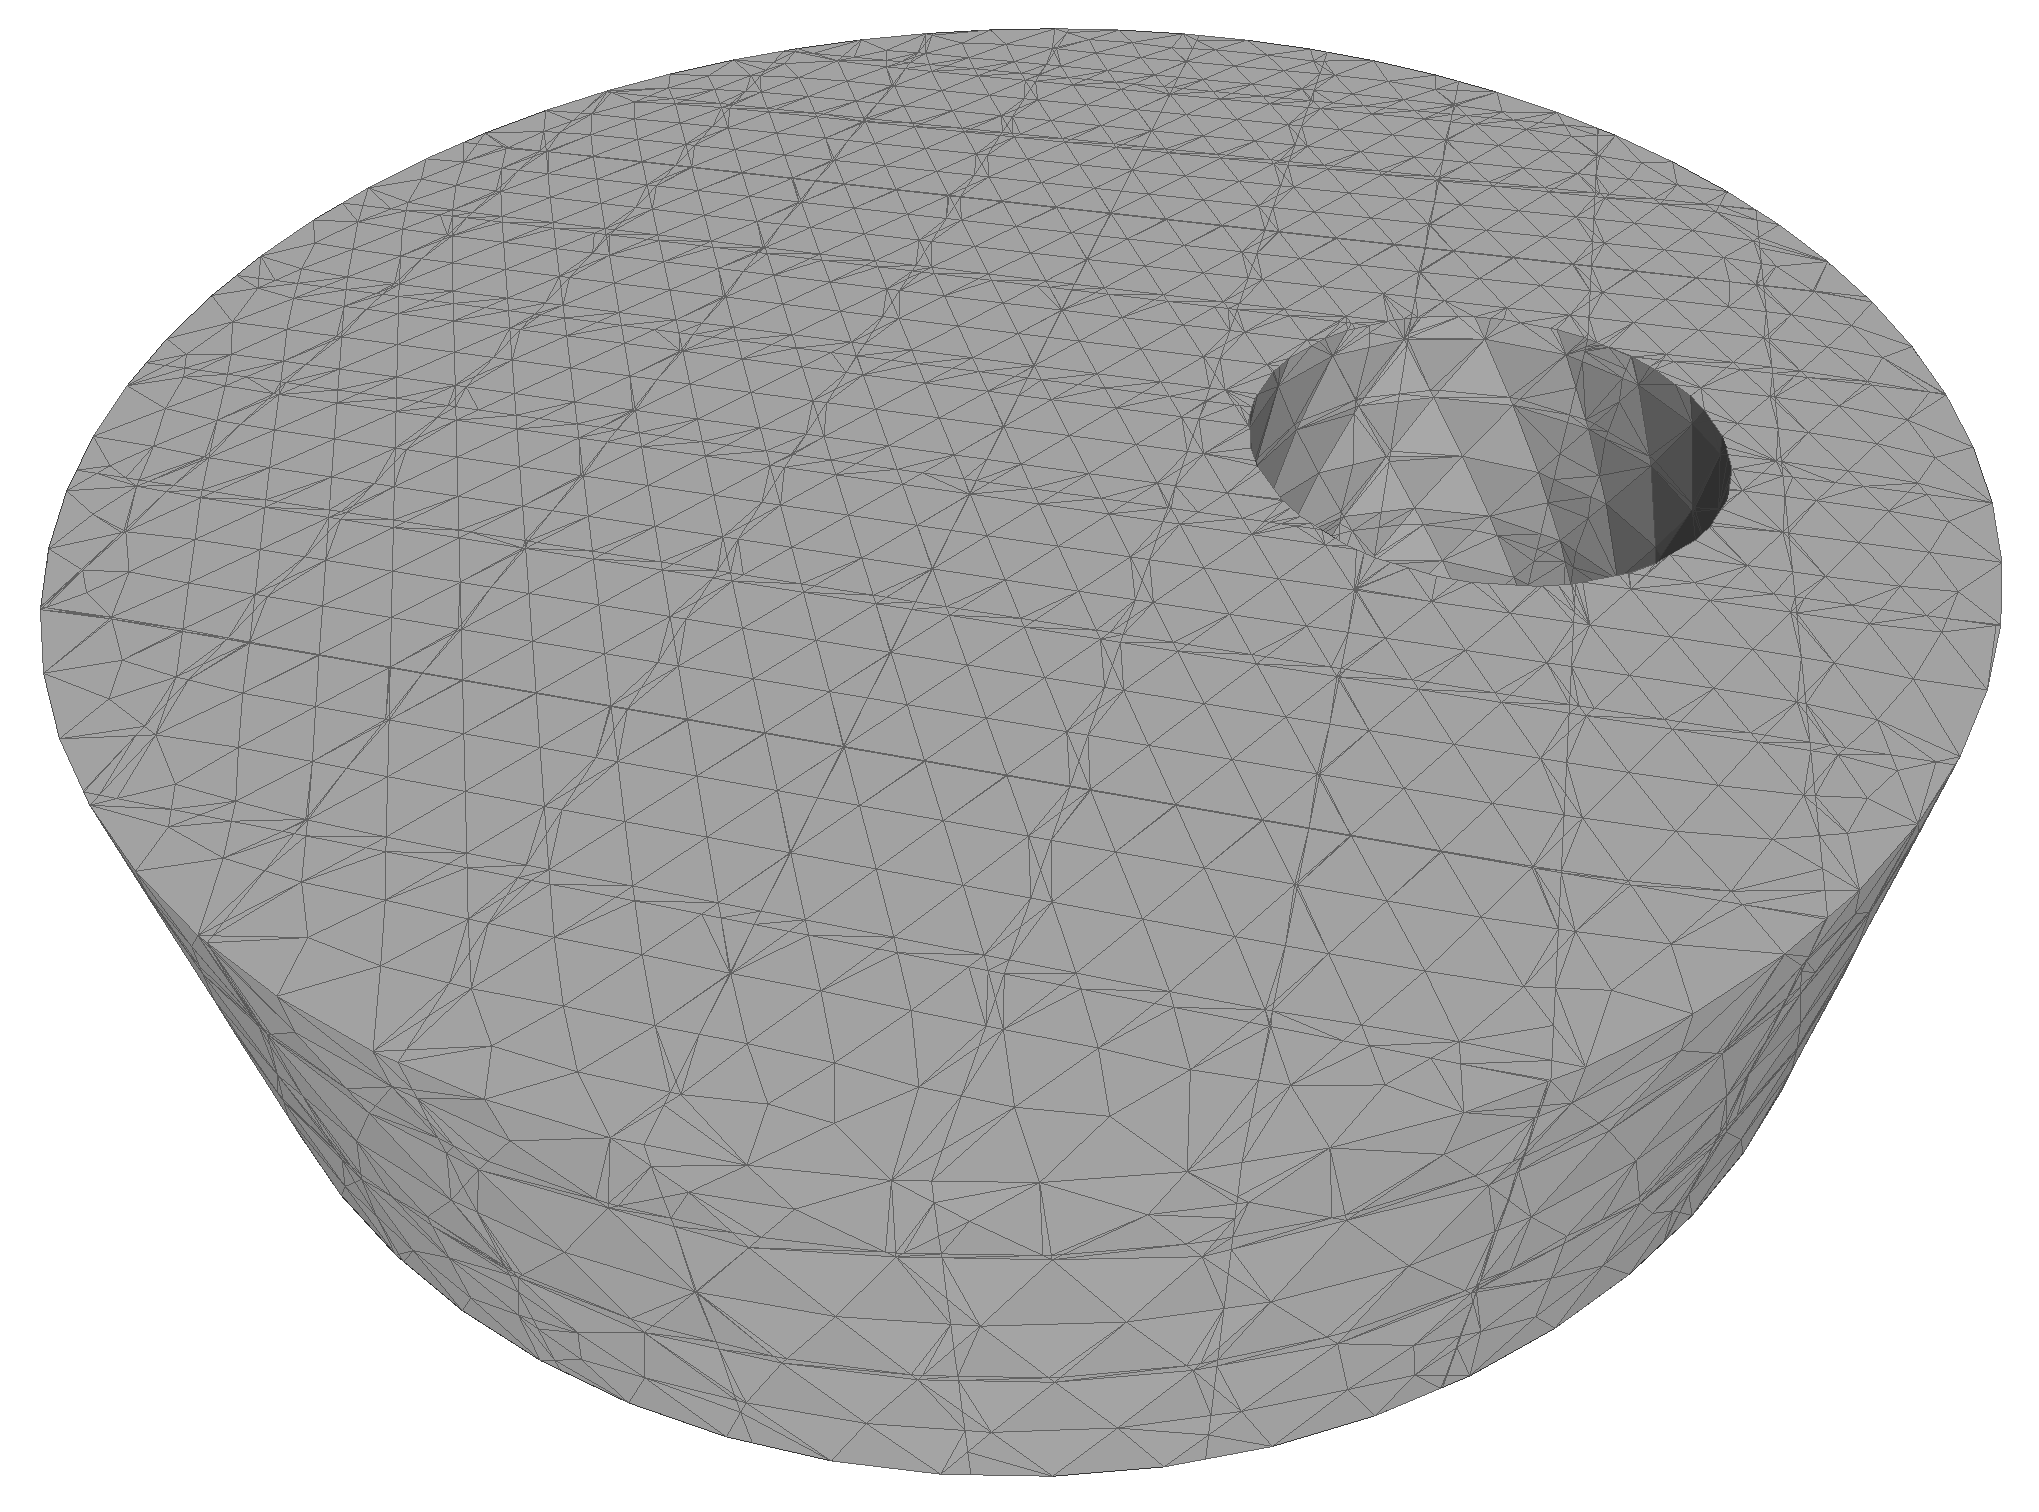
\includegraphics[width=\textwidth]{di_cylinders_delaunay}
		\caption{\cylindersd}
		\label{fig:di_cylinders_d}
	\end{subfigure}
	\begin{subfigure}[b]{0.34\textwidth}
		\centering
		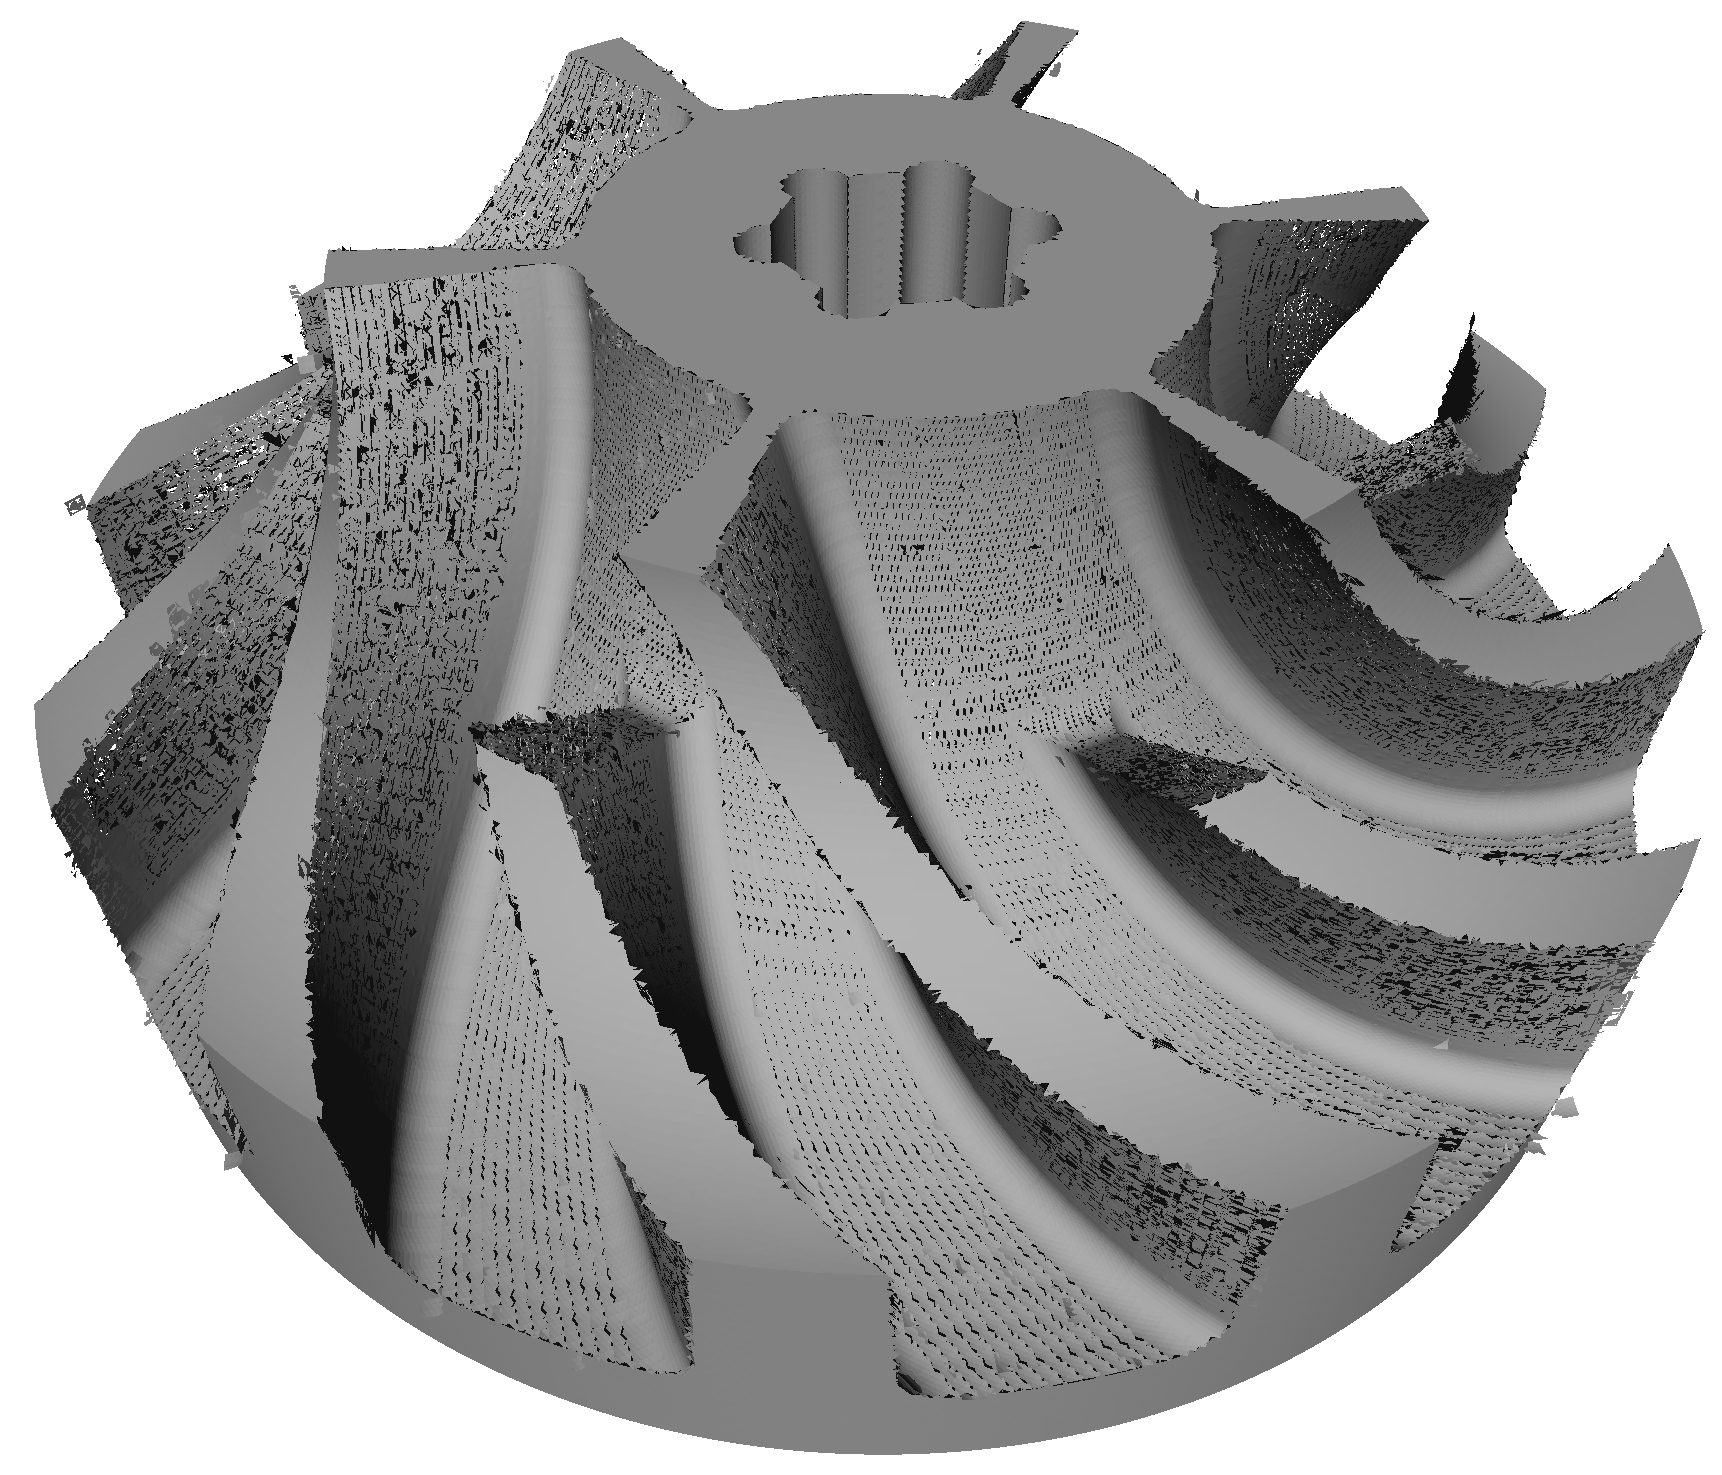
\includegraphics[width=\textwidth]{di_hq_impeller}
		\caption{\impeller}
		\label{fig:di_impeller}
	\end{subfigure}
	\hspace{1cm}
	\begin{subfigure}[b]{0.34\textwidth}
		\centering
		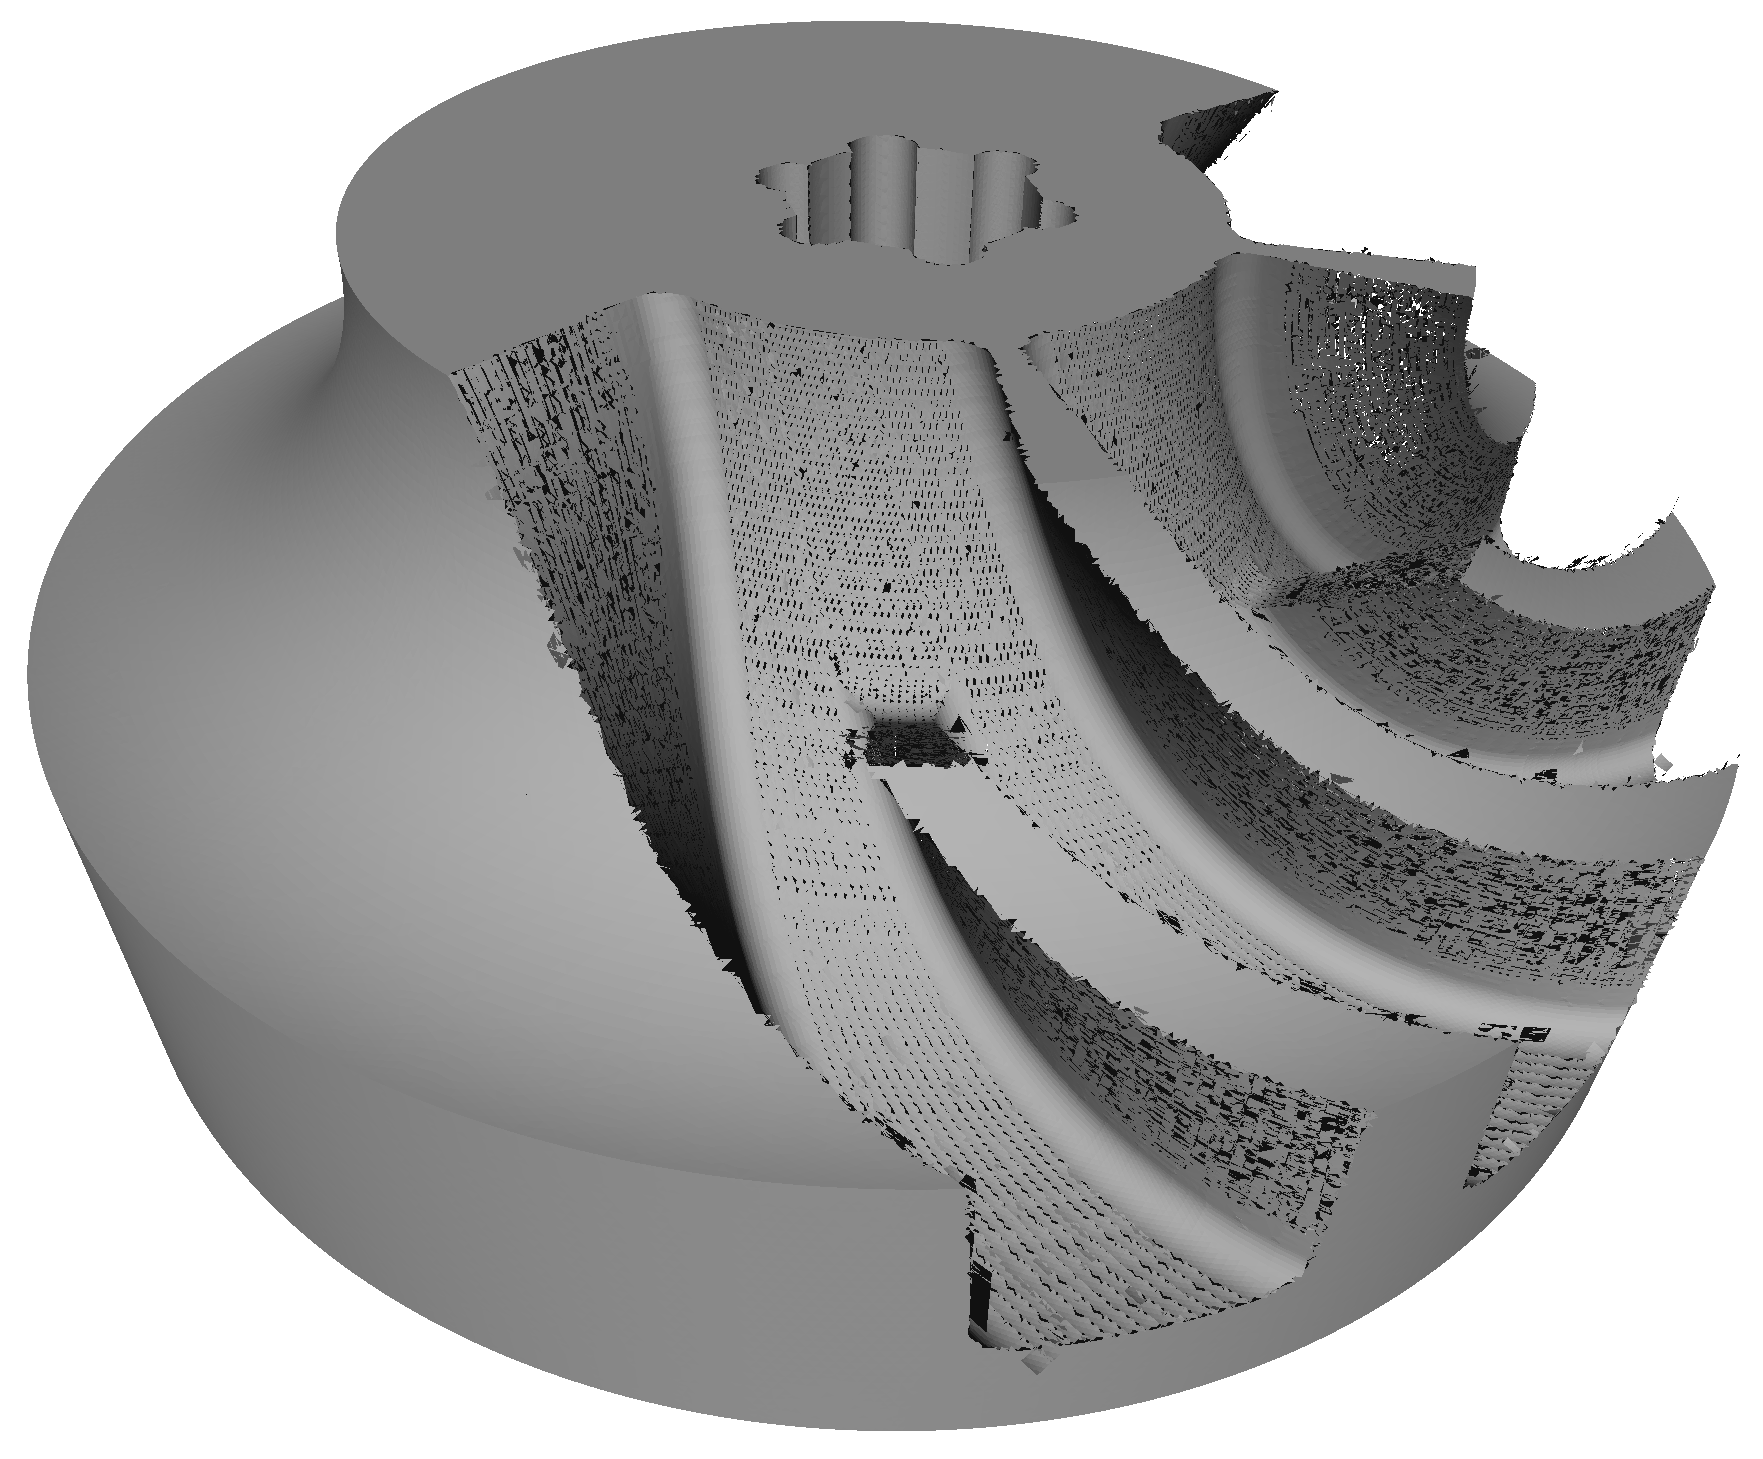
\includegraphics[width=\textwidth]{di_hq_impeller_2}
		\caption{\impellerhalf}
		\label{fig:di_impeller_2}
	\end{subfigure}
	\begin{subfigure}[b]{0.33\textwidth}
		\centering
		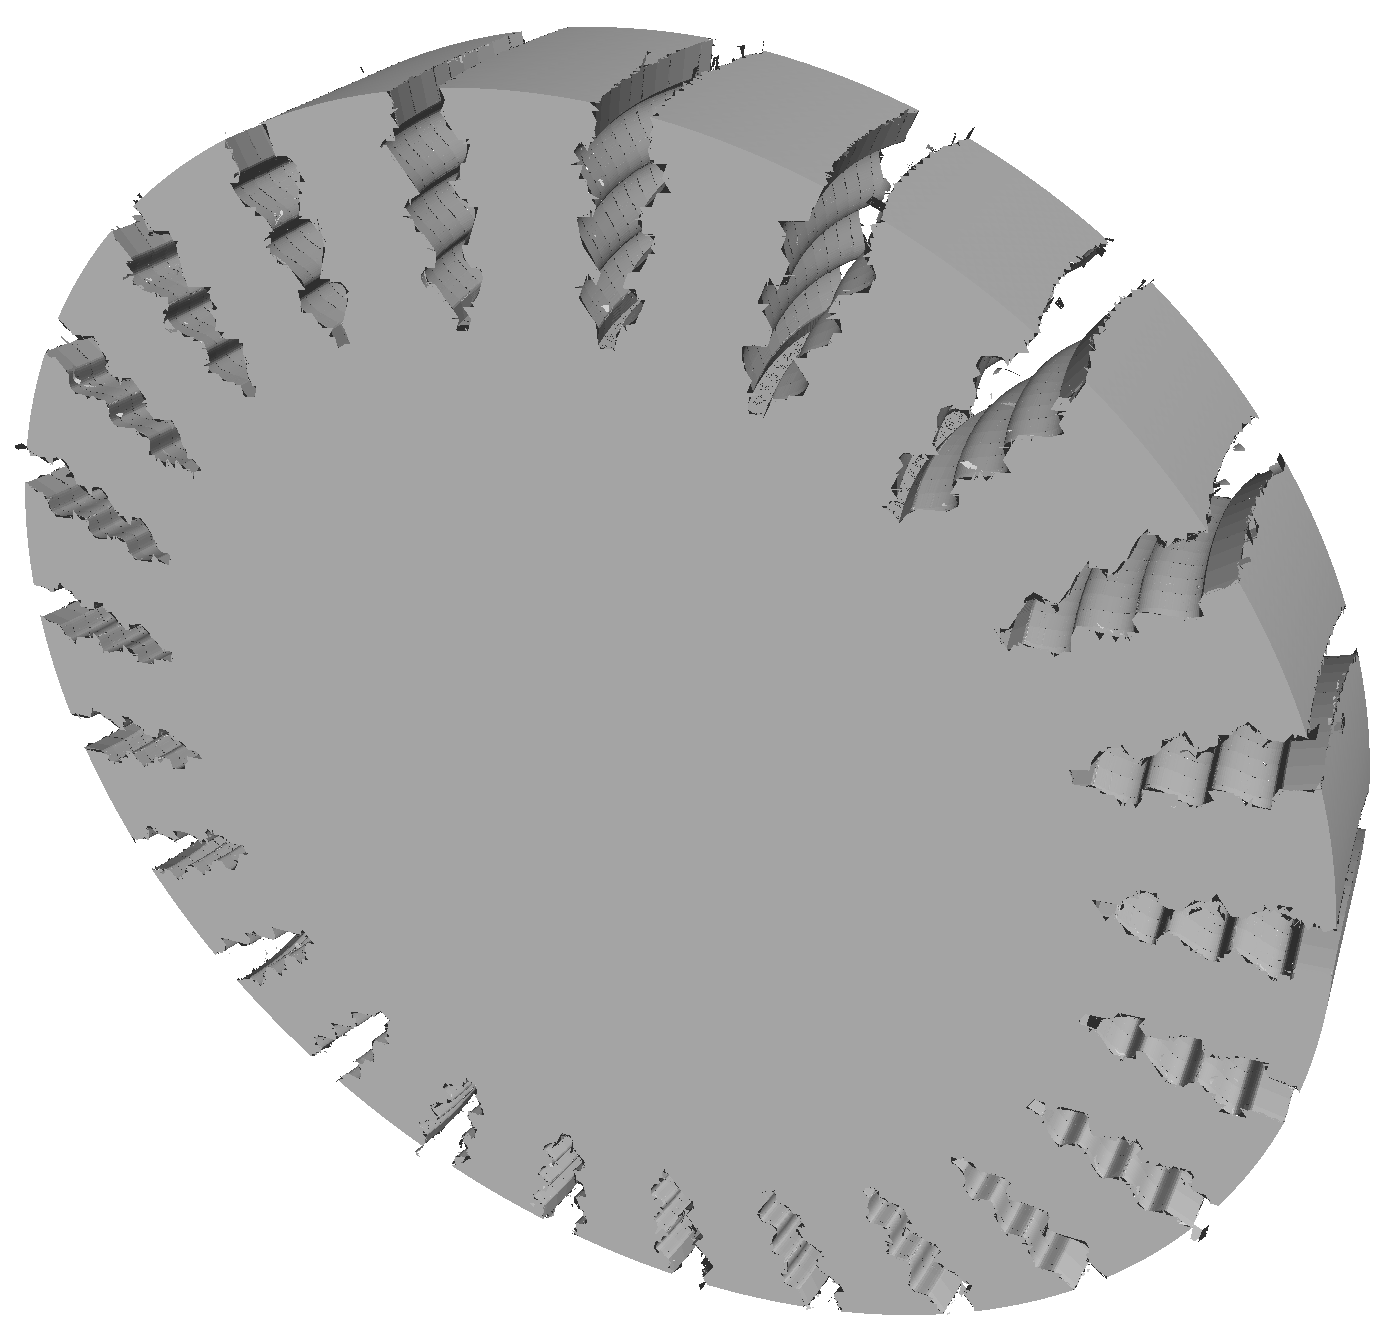
\includegraphics[width=\textwidth]{di_turbine}
		\caption{\turbine}
		\label{fig:di_turbine}
	\end{subfigure}
	\caption[Direct intersection result renderings]{
		Renderings of the result meshes after applying the direct intersection reconstruction approach on the selected test scenes in \cref{tbl:test_scenes}.
	}
	\label{fig:di_results}
\end{figure}

\Cref{fig:di_scenes_artifacts} shows two detailed views, one centered on a smaller blade of the \impeller and one centered on a milling groove of the \turbine.

\begin{figure}
	\centering
	\begin{subfigure}[b]{\textwidth}
		\centering
		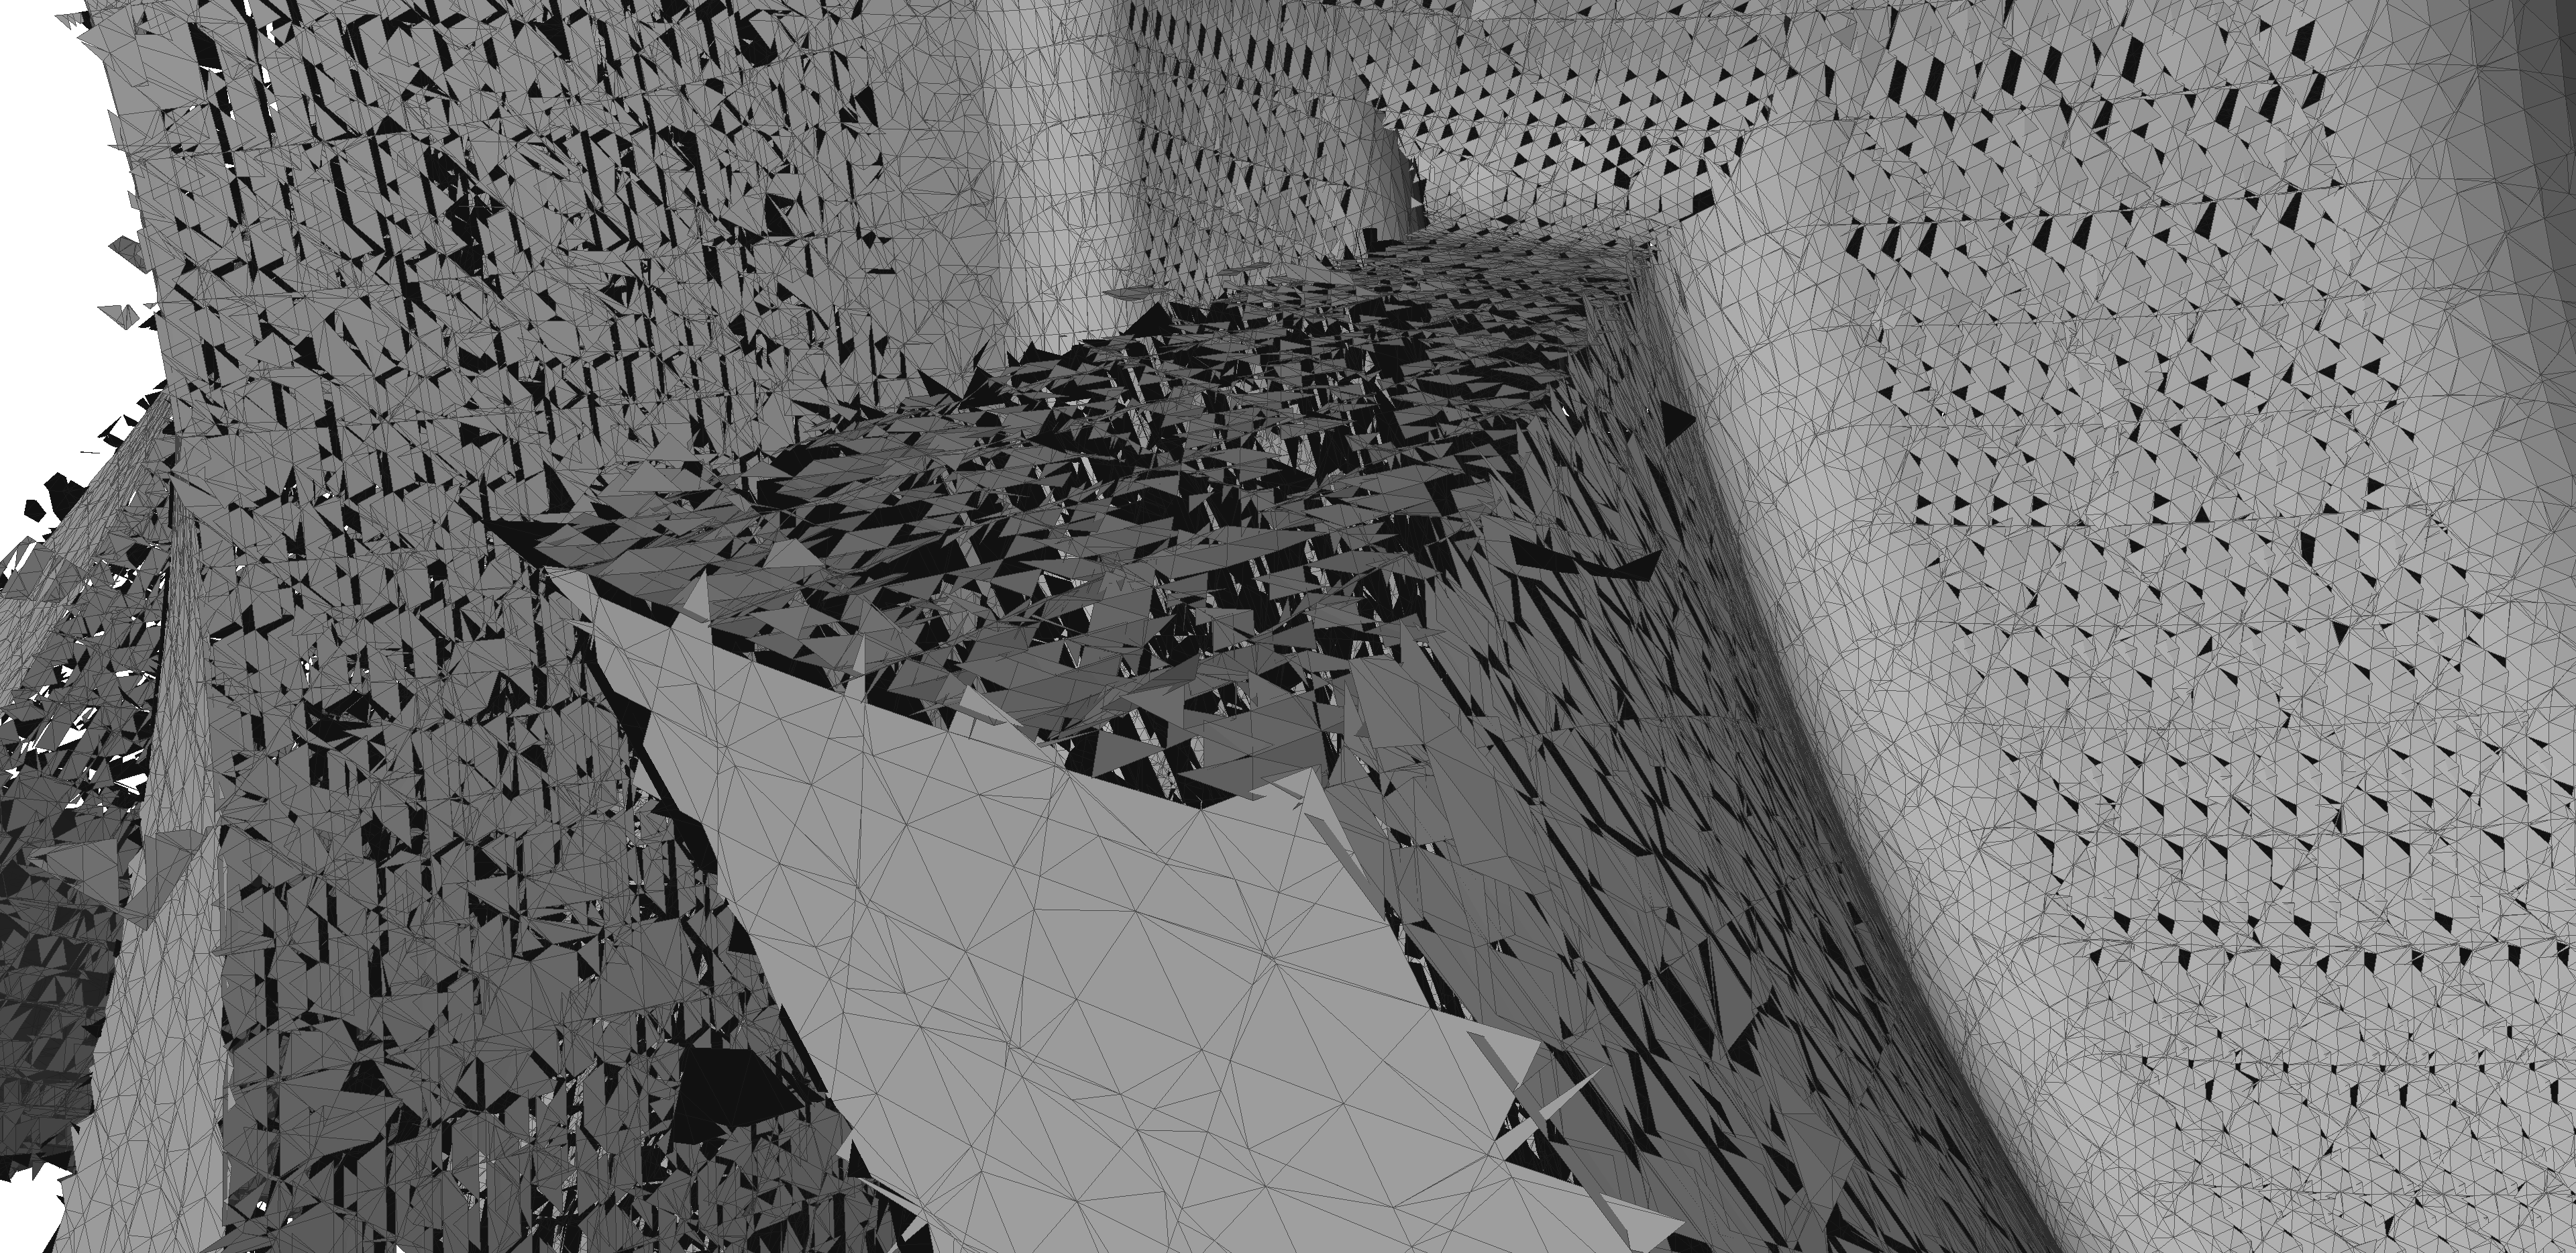
\includegraphics[width=0.8\textwidth]{di_hq_impeller_detail}
		\caption{\impeller}
		\label{fig:di_impeller_detail}
	\end{subfigure}\\
	\begin{subfigure}[b]{\textwidth}
		\centering
		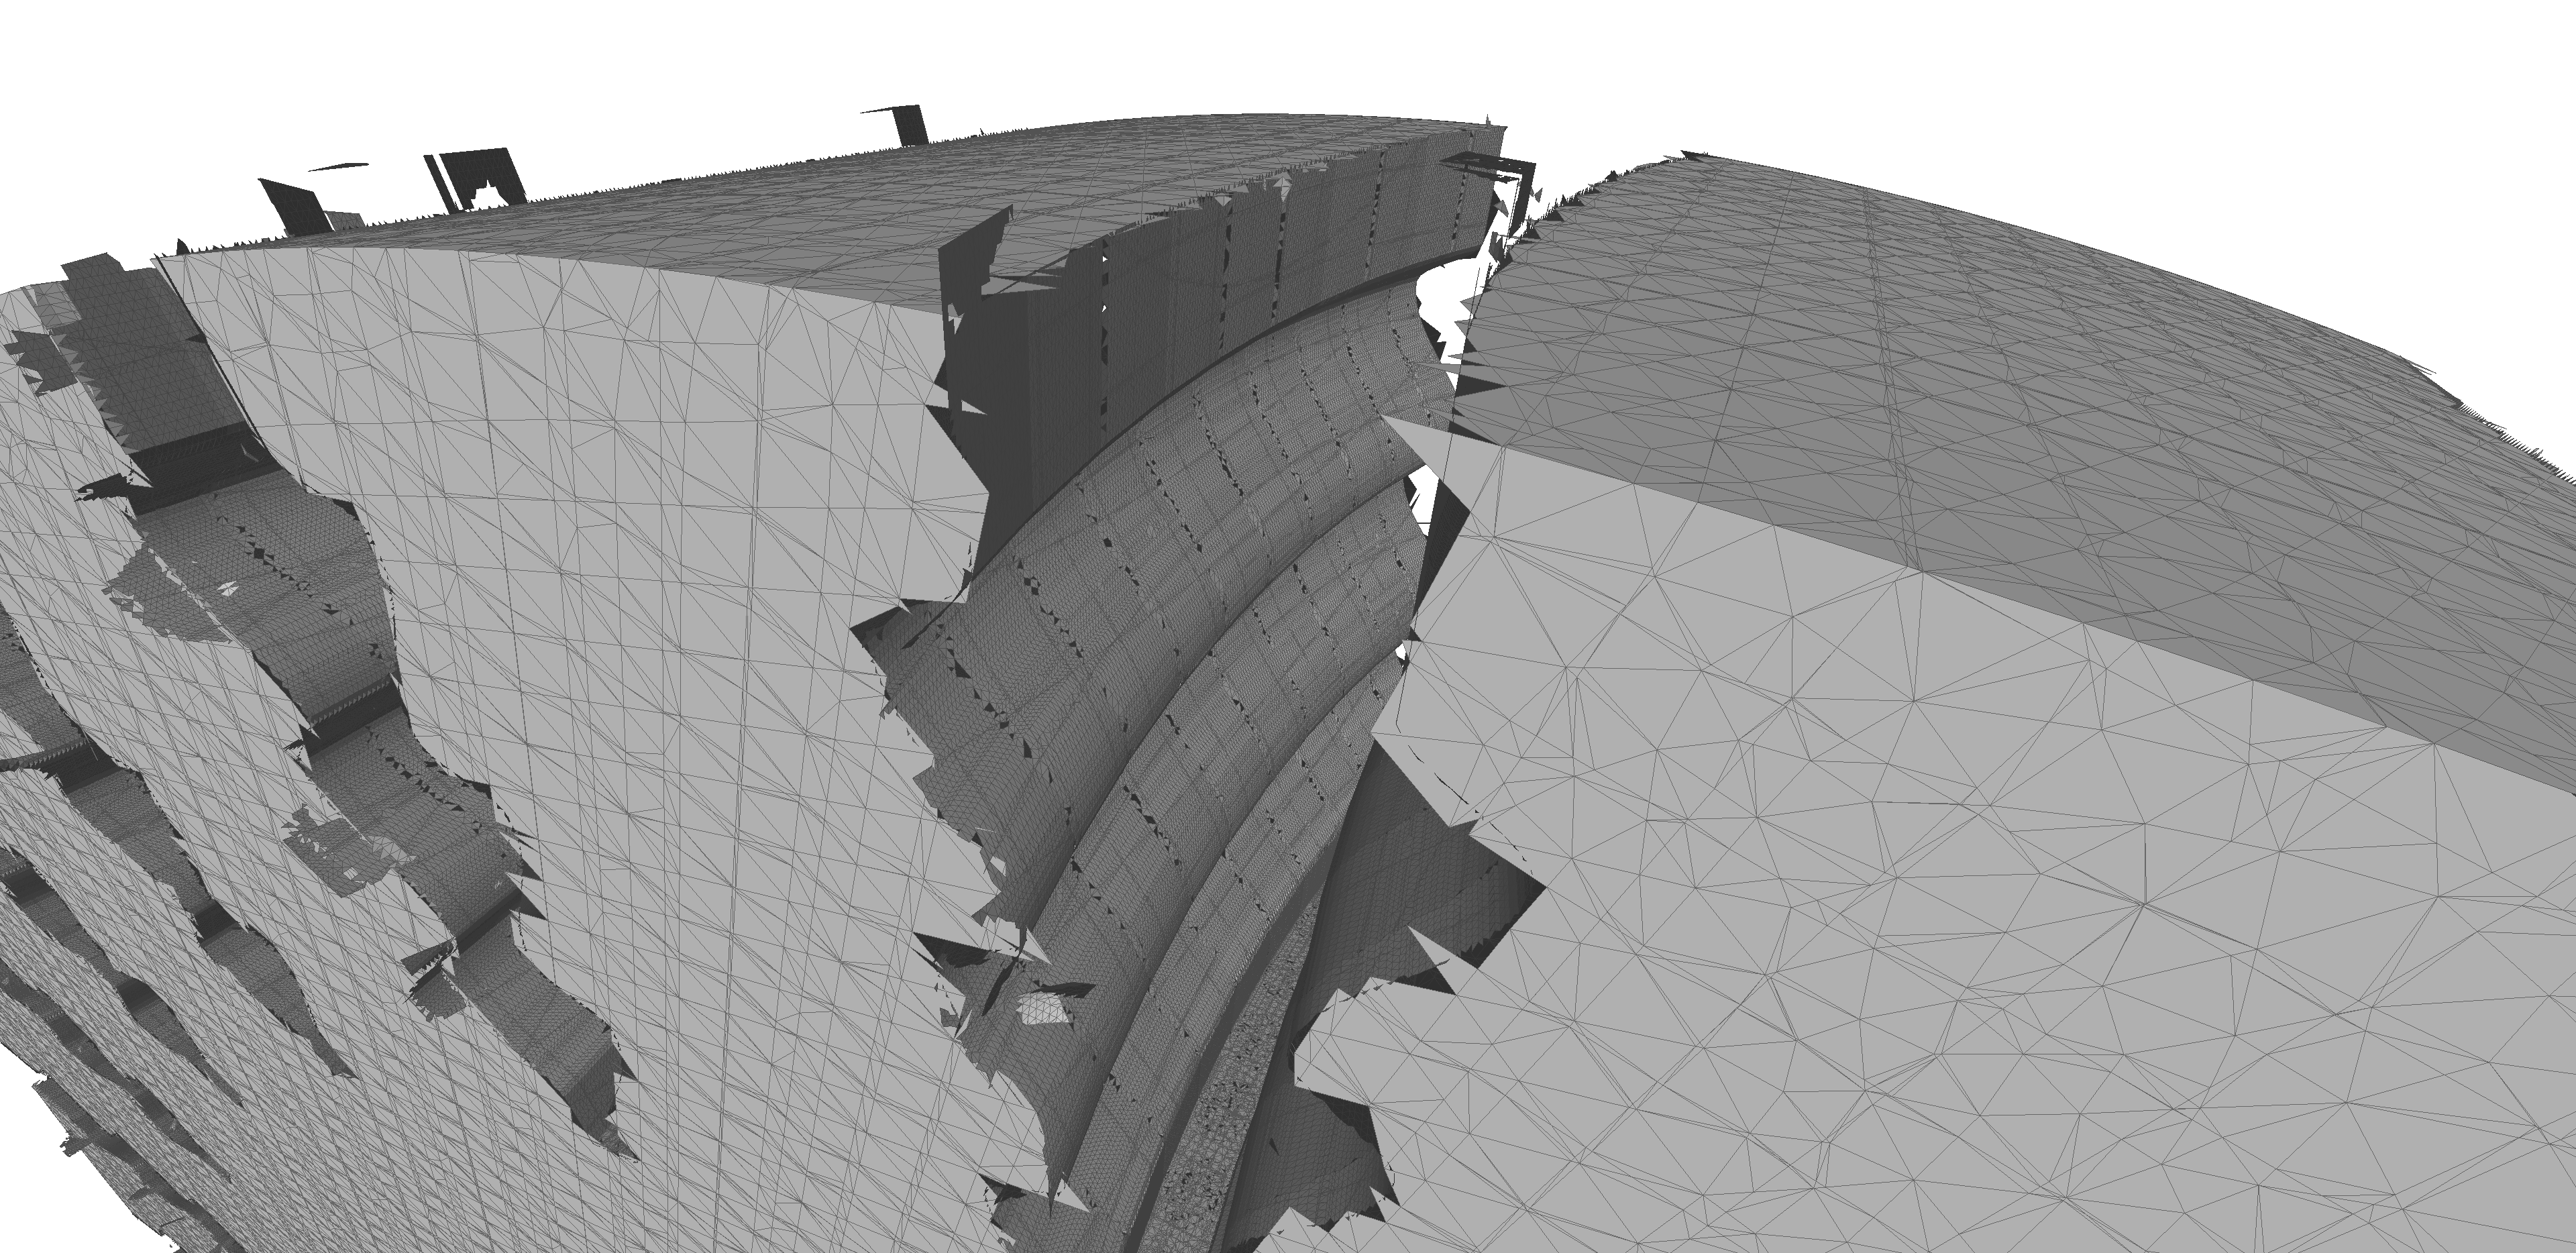
\includegraphics[width=0.8\textwidth]{di_turbine_detail}
		\caption{\turbine}
		\label{fig:di_turbine_detail}
	\end{subfigure}
	\caption[Direct intersection artifacts]{
		Renderings of selected areas from the \impeller \subref{fig:di_impeller_detail} and \turbine \subref{fig:di_turbine_detail} scene after applying the direct intersection reconstruction approach.
	}
	\label{fig:di_scenes_artifacts}
\end{figure}

The created boundary edges are listed in \cref{tbl:direct_intersection_boundary_edges}.

\begin{table}
	\centering
	\begin{tabular}{l|r}
		scene         &  boundary edges         \\
		\midrule
		\cubes        & \SI{ 75}{     \nothing} \\
		\cylindersd   & \SI{ 69}{     \nothing} \\
		\cylinders    & \SI{  1}{\kilo\nothing} \\ %   1078
		\cylinderhead & \SI{ 22}{\kilo\nothing} \\ %  22432
		\impeller     & \SI{660}{\kilo\nothing} \\ % 659695
		\impellerhalf & \SI{326}{\kilo\nothing} \\ % 326171
		\turbine      & \SI{402}{\kilo\nothing} \\ % 401917
	\end{tabular}
	\caption[Direct intersection boundary edges]{
		Created boundary edges by the direct intersection surface extraction.
	}
	\label{tbl:direct_intersection_boundary_edges}
\end{table}


\section{Tri-dexel}
\label{sec:tri_dexel_results}

For testing the tri-dexel surface reconstruction approach, \cf \cref{ch:tri_dexel}, a few different grid resolutions have been used, which are 50, 100, 200 and 400.
\Cref{tbl:tri_dexel_results} contains the runtime and output size of the test runs.

\begin{table}
	\begin{subtable}{\textwidth}
		\centering
		\begin{tabular}{l|rr|rr|rr|rr}
			resolution    & \multicolumn{2}{c}{50} & \multicolumn{2}{c}{100} & \multicolumn{2}{c}{200} & \multicolumn{2}{c}{400} \\
			scene         & t\sub{out} & time & t\sub{out} & time & t\sub{out} & time & t\sub{out} & time \\
			\midrule
			\cubes        & \SI{55}{\kilo\nothing} & \SI{137}{\milli\second} & \SI{222}{\kilo\nothing} & \SI{1.1}{\second} & \SI{901}{\kilo\nothing} & \SI{10.5}{\second} & \SI{3.6}{\mega\nothing} & \SI{203}{\second} \\
			\cylindersd   & \SI{33}{\kilo\nothing} & \SI{ 39}{\milli\second} & \SI{112}{\kilo\nothing} & \SI{0.3}{\second} & \SI{436}{\kilo\nothing} & \SI{ 2.1}{\second} & \SI{1.7}{\mega\nothing} & \SI{ 27}{\second} \\
			\cylinders    & \SI{30}{\kilo\nothing} & \SI{ 34}{\milli\second} & \SI{112}{\kilo\nothing} & \SI{0.3}{\second} & \SI{435}{\kilo\nothing} & \SI{ 2.1}{\second} & \SI{1.7}{\mega\nothing} & \SI{ 26}{\second} \\
			\cylinderhead & \SI{74}{\kilo\nothing} & \SI{ 56}{\milli\second} & \SI{263}{\kilo\nothing} & \SI{0.4}{\second} & \SI{965}{\kilo\nothing} & \SI{ 2.9}{\second} & \SI{3.8}{\mega\nothing} & \SI{ 32}{\second} \\
			\impeller     & \SI{76}{\kilo\nothing} & \SI{135}{\milli\second} & \SI{242}{\kilo\nothing} & \SI{0.6}{\second} & \SI{853}{\kilo\nothing} & \SI{ 3.3}{\second} & \SI{3.0}{\mega\nothing} & \SI{ 27}{\second} \\
			\impellerhalf & \SI{62}{\kilo\nothing} & \SI{ 95}{\milli\second} & \SI{195}{\kilo\nothing} & \SI{0.5}{\second} & \SI{696}{\kilo\nothing} & \SI{ 3.1}{\second} & \SI{2.5}{\mega\nothing} & \SI{ 31}{\second} \\
			\turbine      & \SI{38}{\kilo\nothing} & \SI{179}{\milli\second} & \SI{162}{\kilo\nothing} & \SI{0.8}{\second} & \SI{629}{\kilo\nothing} & \SI{ 3.7}{\second} & \SI{2.3}{\mega\nothing} & \SI{ 21}{\second} \\
		\end{tabular}
		\caption{
			without cell slicing.
		}
		\label{tbl:tri_dexel_results_no_slicing}
	\end{subtable}
	\bigskip\\
	\begin{subtable}{\textwidth}
		\centering
		\begin{tabular}{l|rr|rr|rr|rr}
			resolution    & \multicolumn{2}{c}{50} & \multicolumn{2}{c}{100} & \multicolumn{2}{c}{200} & \multicolumn{2}{c}{400} \\
			scene         & t\sub{out} & time & t\sub{out} & time & t\sub{out} & time & t\sub{out} & time \\
			\midrule
			\cubes        & \SI{55}{\kilo\nothing} & \SI{ 138}{\milli\second} & \SI{222}{\kilo\nothing} & \SI{1.1}{\second} & \SI{901}{\kilo\nothing} & \SI{10.5}{\second} & \SI{3.6}{\mega\nothing} & \SI{198}{\second} \\
			\cylindersd   & \SI{33}{\kilo\nothing} & \SI{  38}{\milli\second} & \SI{113}{\kilo\nothing} & \SI{0.3}{\second} & \SI{436}{\kilo\nothing} & \SI{ 2.1}{\second} & \SI{1.7}{\mega\nothing} & \SI{ 27}{\second} \\
			\cylinders    & \SI{30}{\kilo\nothing} & \SI{  33}{\milli\second} & \SI{112}{\kilo\nothing} & \SI{0.3}{\second} & \SI{435}{\kilo\nothing} & \SI{ 2.1}{\second} & \SI{1.7}{\mega\nothing} & \SI{ 26}{\second} \\
			\cylinderhead & \SI{81}{\kilo\nothing} & \SI{ 102}{\milli\second} & \SI{276}{\kilo\nothing} & \SI{0.5}{\second} & \SI{988}{\kilo\nothing} & \SI{ 3.0}{\second} & \SI{3.8}{\mega\nothing} & \SI{ 32}{\second} \\
			\impeller     & \SI{82}{\kilo\nothing} & \SI{ 743}{\milli\second} & \SI{252}{\kilo\nothing} & \SI{1.8}{\second} & \SI{872}{\kilo\nothing} & \SI{ 6.3}{\second} & \SI{3.0}{\mega\nothing} & \SI{ 51}{\second} \\
			\impellerhalf & \SI{66}{\kilo\nothing} & \SI{ 358}{\milli\second} & \SI{200}{\kilo\nothing} & \SI{1.0}{\second} & \SI{708}{\kilo\nothing} & \SI{ 3.9}{\second} & \SI{2.5}{\mega\nothing} & \SI{ 38}{\second} \\
			\turbine      & \SI{47}{\kilo\nothing} & \SI{3068}{\milli\second} & \SI{180}{\kilo\nothing} & \SI{8.1}{\second} & \SI{657}{\kilo\nothing} & \SI{23.5}{\second} & \SI{2.3}{\mega\nothing} & \SI{145}{\second} \\
		\end{tabular}
		\caption{
			with cell slicing.
		}
		\label{tbl:tri_dexel_results_slicing}
	\end{subtable}
	\caption[Tri-dexel results]{
		Test results for the tri-dexel surface extraction approach without and with one recursion of cell slicing.
	}
	\label{tbl:tri_dexel_results}
\end{table}

The CPU utilization during a single run of the tri-dexel surface extraction of the \impeller scene with a grid resolution of 400 is shown in \cref{fig:td_hq_impeller_cpu}.

\begin{figure}
	\centering
	\begin{tikzpicture}
	\begin{axis}[
		width=0.95\textwidth,
		height=0.5\textwidth,
		xlabel={Wall clock time in \si{\second}},
		ylabel={CPU utilization in \si{\percent}},
		ymin=0,
		ymax=100,
		ytick={0,20,...,100},
		%xtick={0,5,...,100}
	]
	\addplot table [x=time, y=utilization, col sep=comma]{spreadsheets/td_hq_impeller_cpu.csv};
	\end{axis}
	\end{tikzpicture}
	%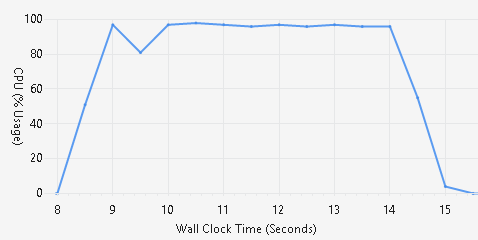
\includegraphics[width=0.9\textwidth]{images/td_hq_impeller_cpu}
	\caption[Tri-dexel CPU utilization]{
		CPU utilization during point cloud creation and a run of the tri-dexel algorithm with a grid resolution of 400, all features enabled, reconstructing the surface of the \impeller scene.
	}
	\label{fig:td_hq_impeller_cpu}
\end{figure}

\Cref{fig:di_results} contains renderings of the resulting triangle meshes.

\begin{figure}
	\centering
	\begin{subfigure}[b]{0.34\textwidth}
		\centering
		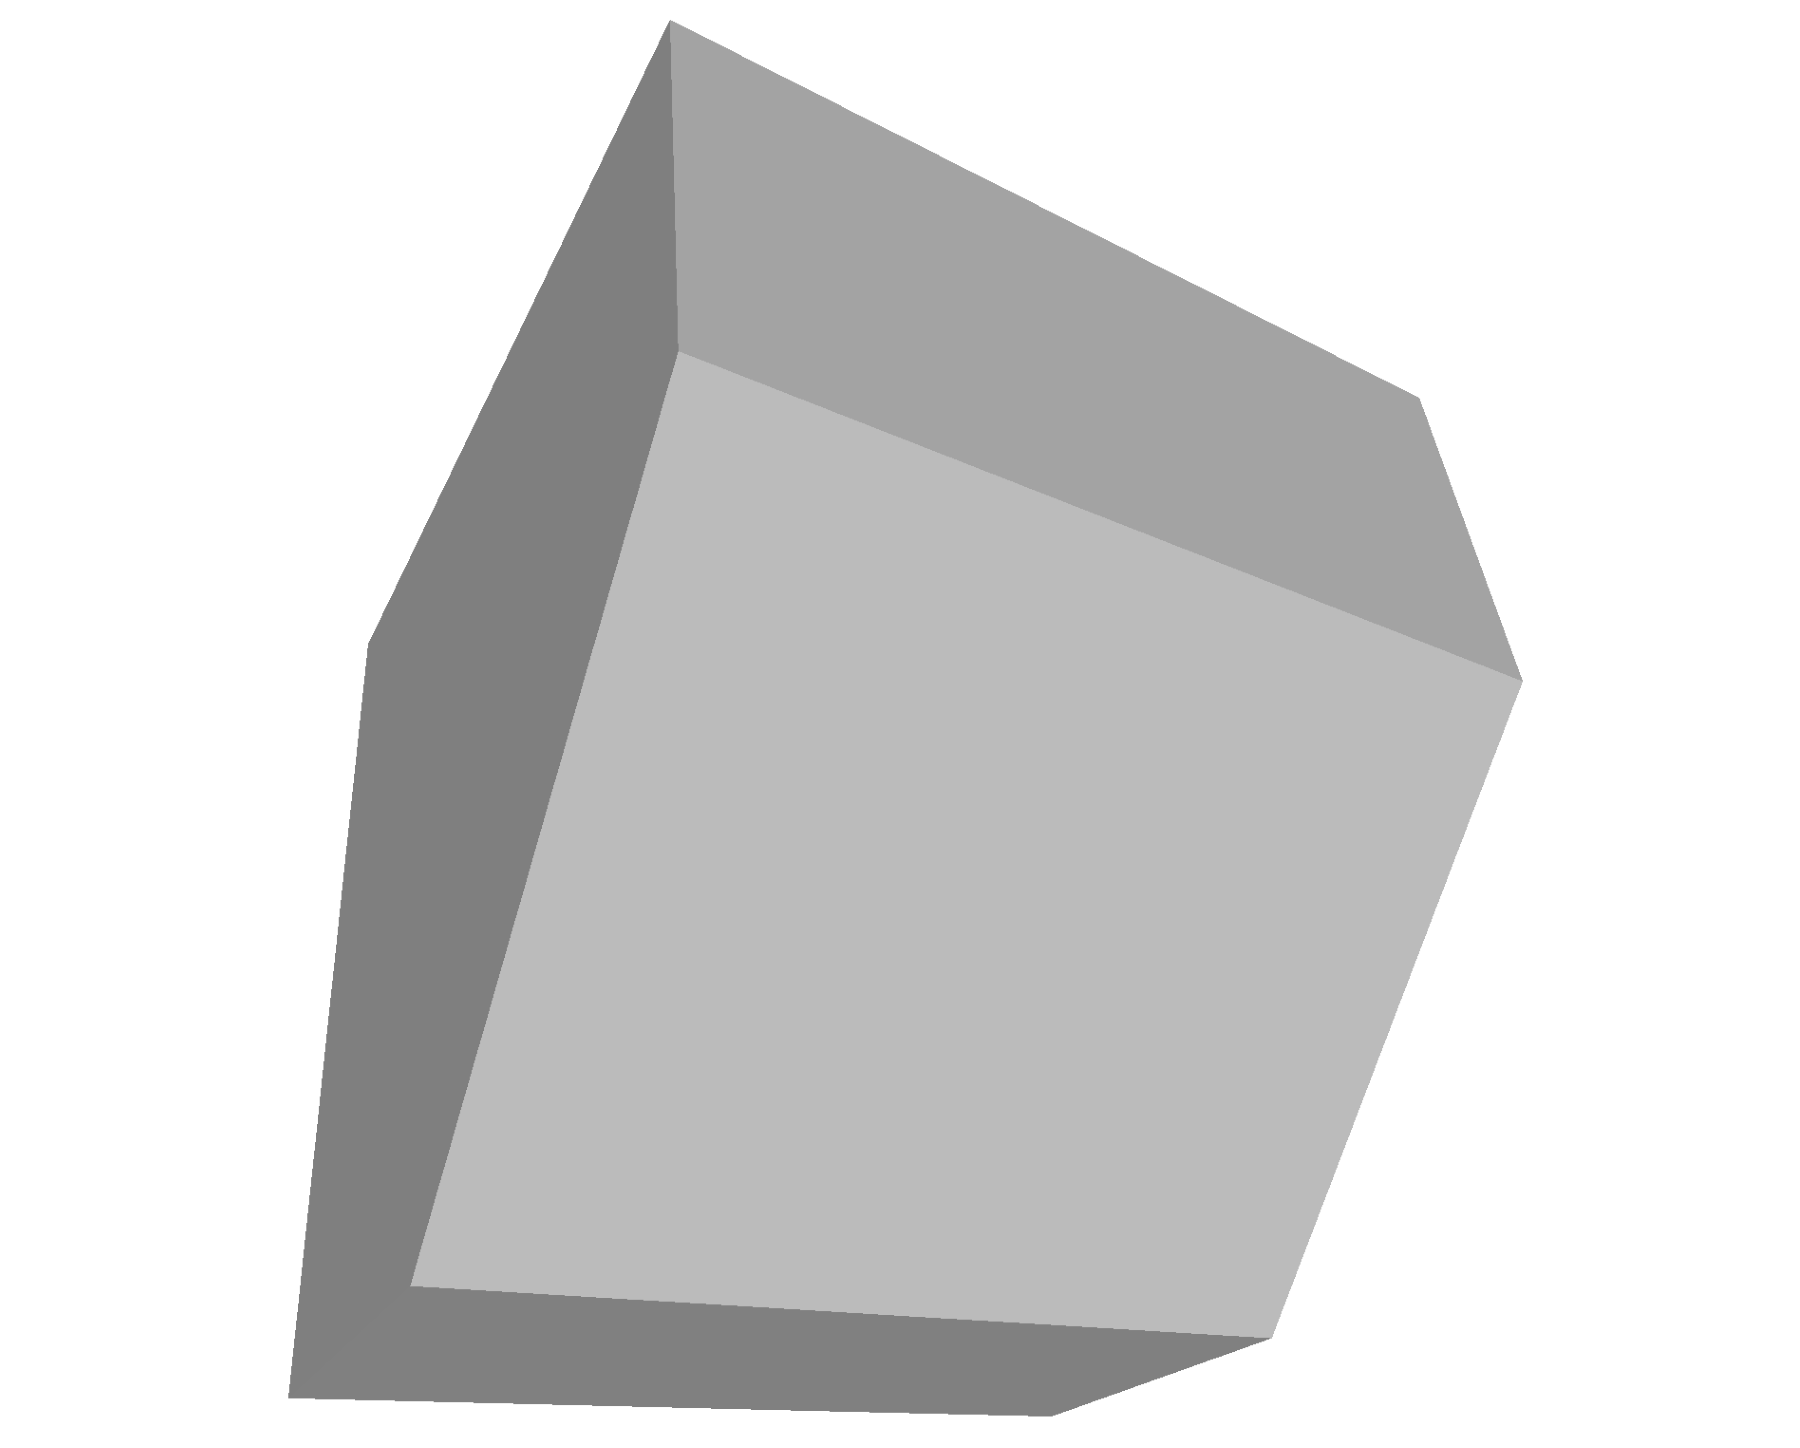
\includegraphics[width=\textwidth]{td_cube2}
		\caption{\cubes}
		\label{fig:td_cube2}
	\end{subfigure}
	\hspace{1cm}
	\begin{subfigure}[b]{0.34\textwidth}
		\centering
		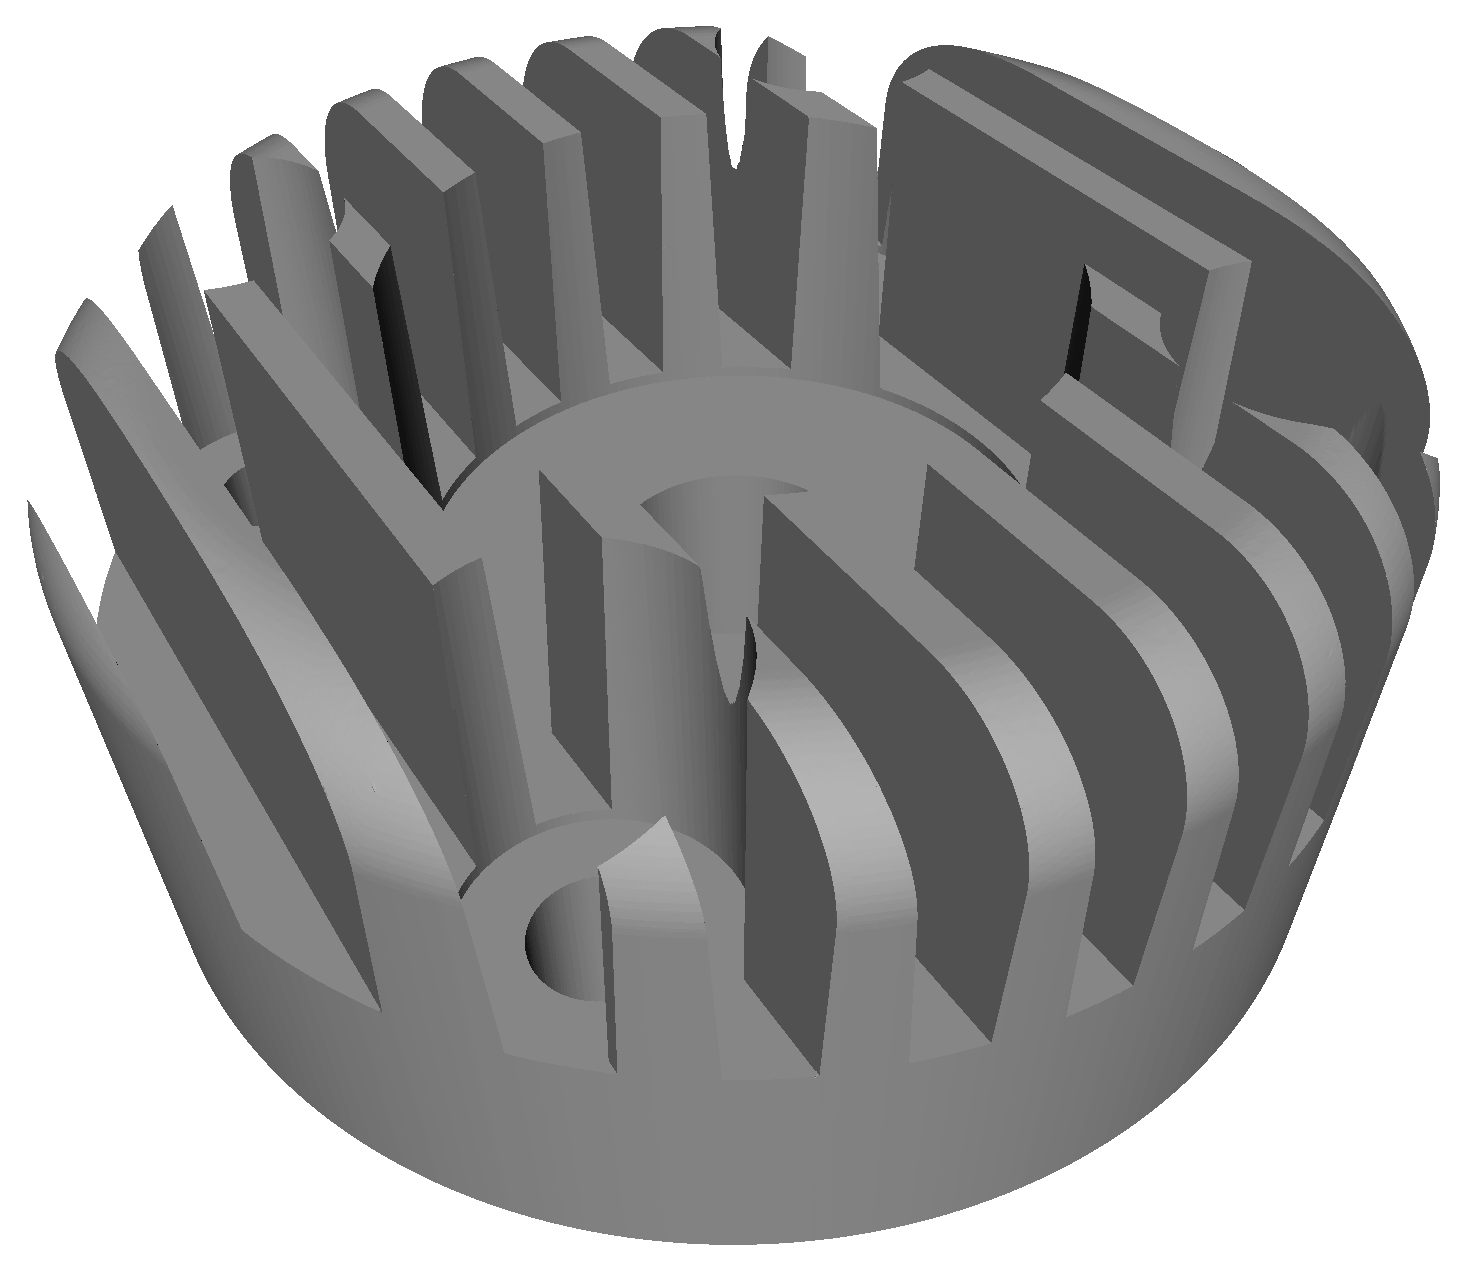
\includegraphics[width=\textwidth]{td_cylinder_head}
		\caption{\cylinderhead}
		\label{fig:td_cylinder_head}
	\end{subfigure}
	\begin{subfigure}[b]{0.34\textwidth}
		\centering
		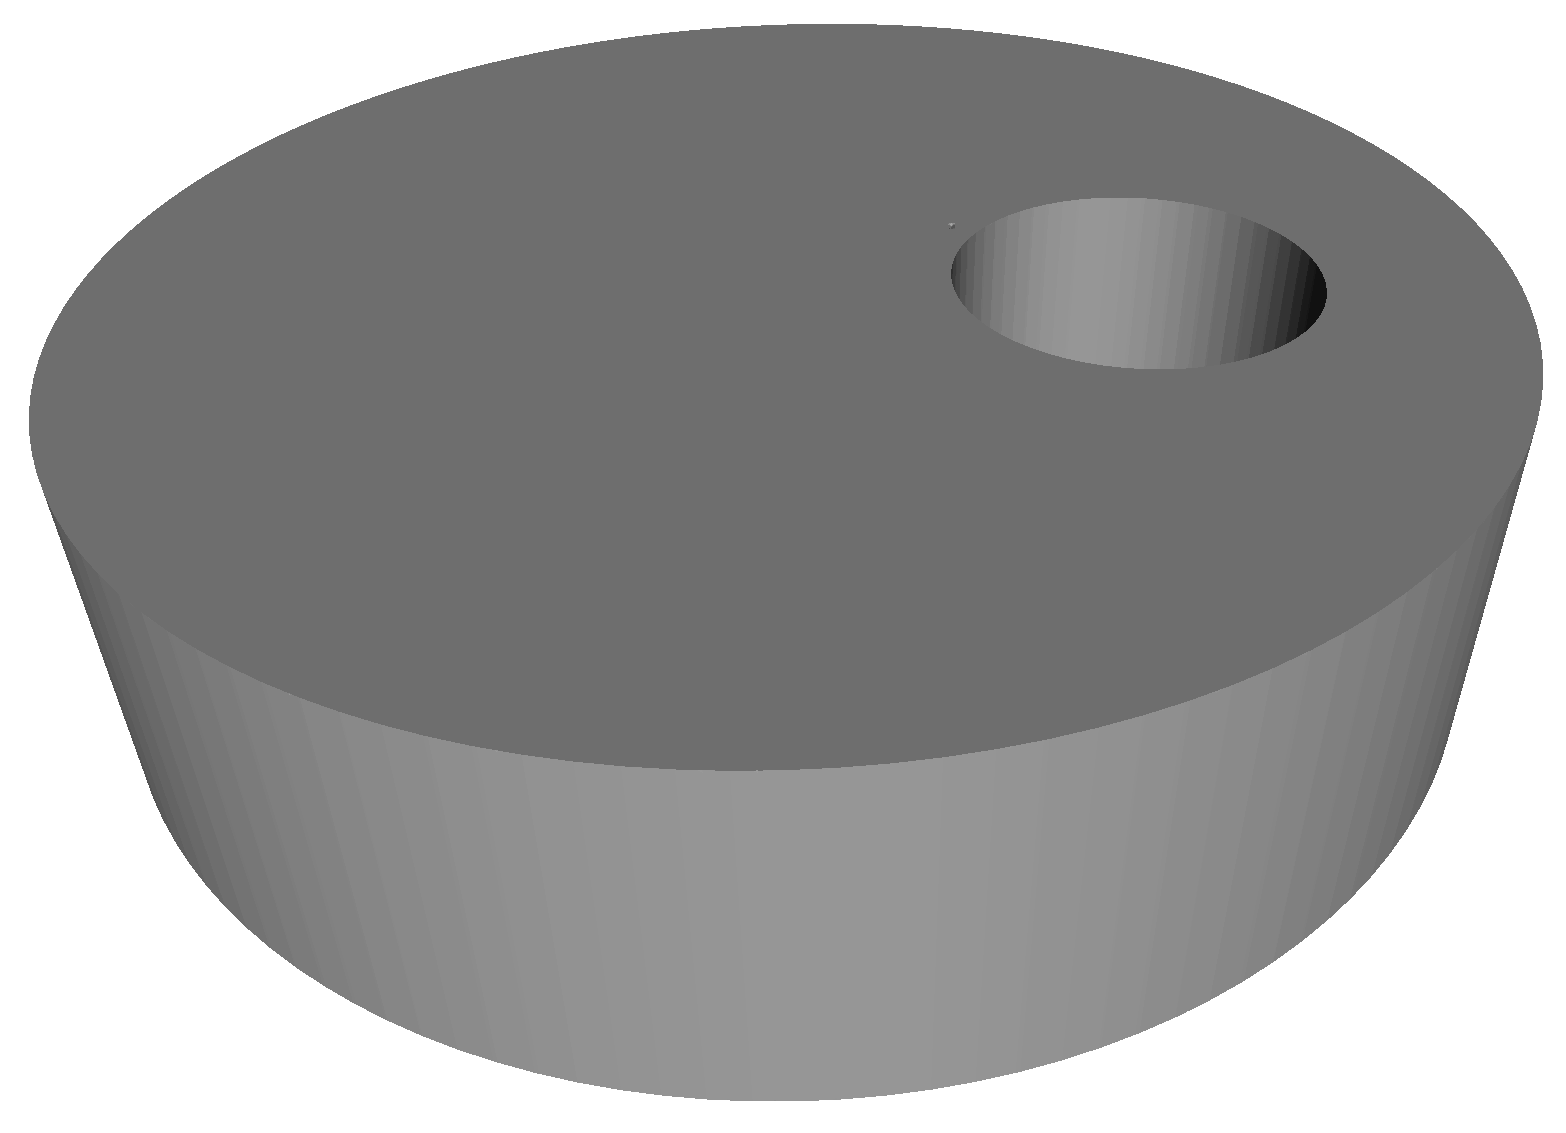
\includegraphics[width=\textwidth]{td_cylinders}
		\caption{\cylinders}
		\label{fig:td_cylinders}
	\end{subfigure}
	\hspace{1cm}
	\begin{subfigure}[b]{0.34\textwidth}
		\centering
		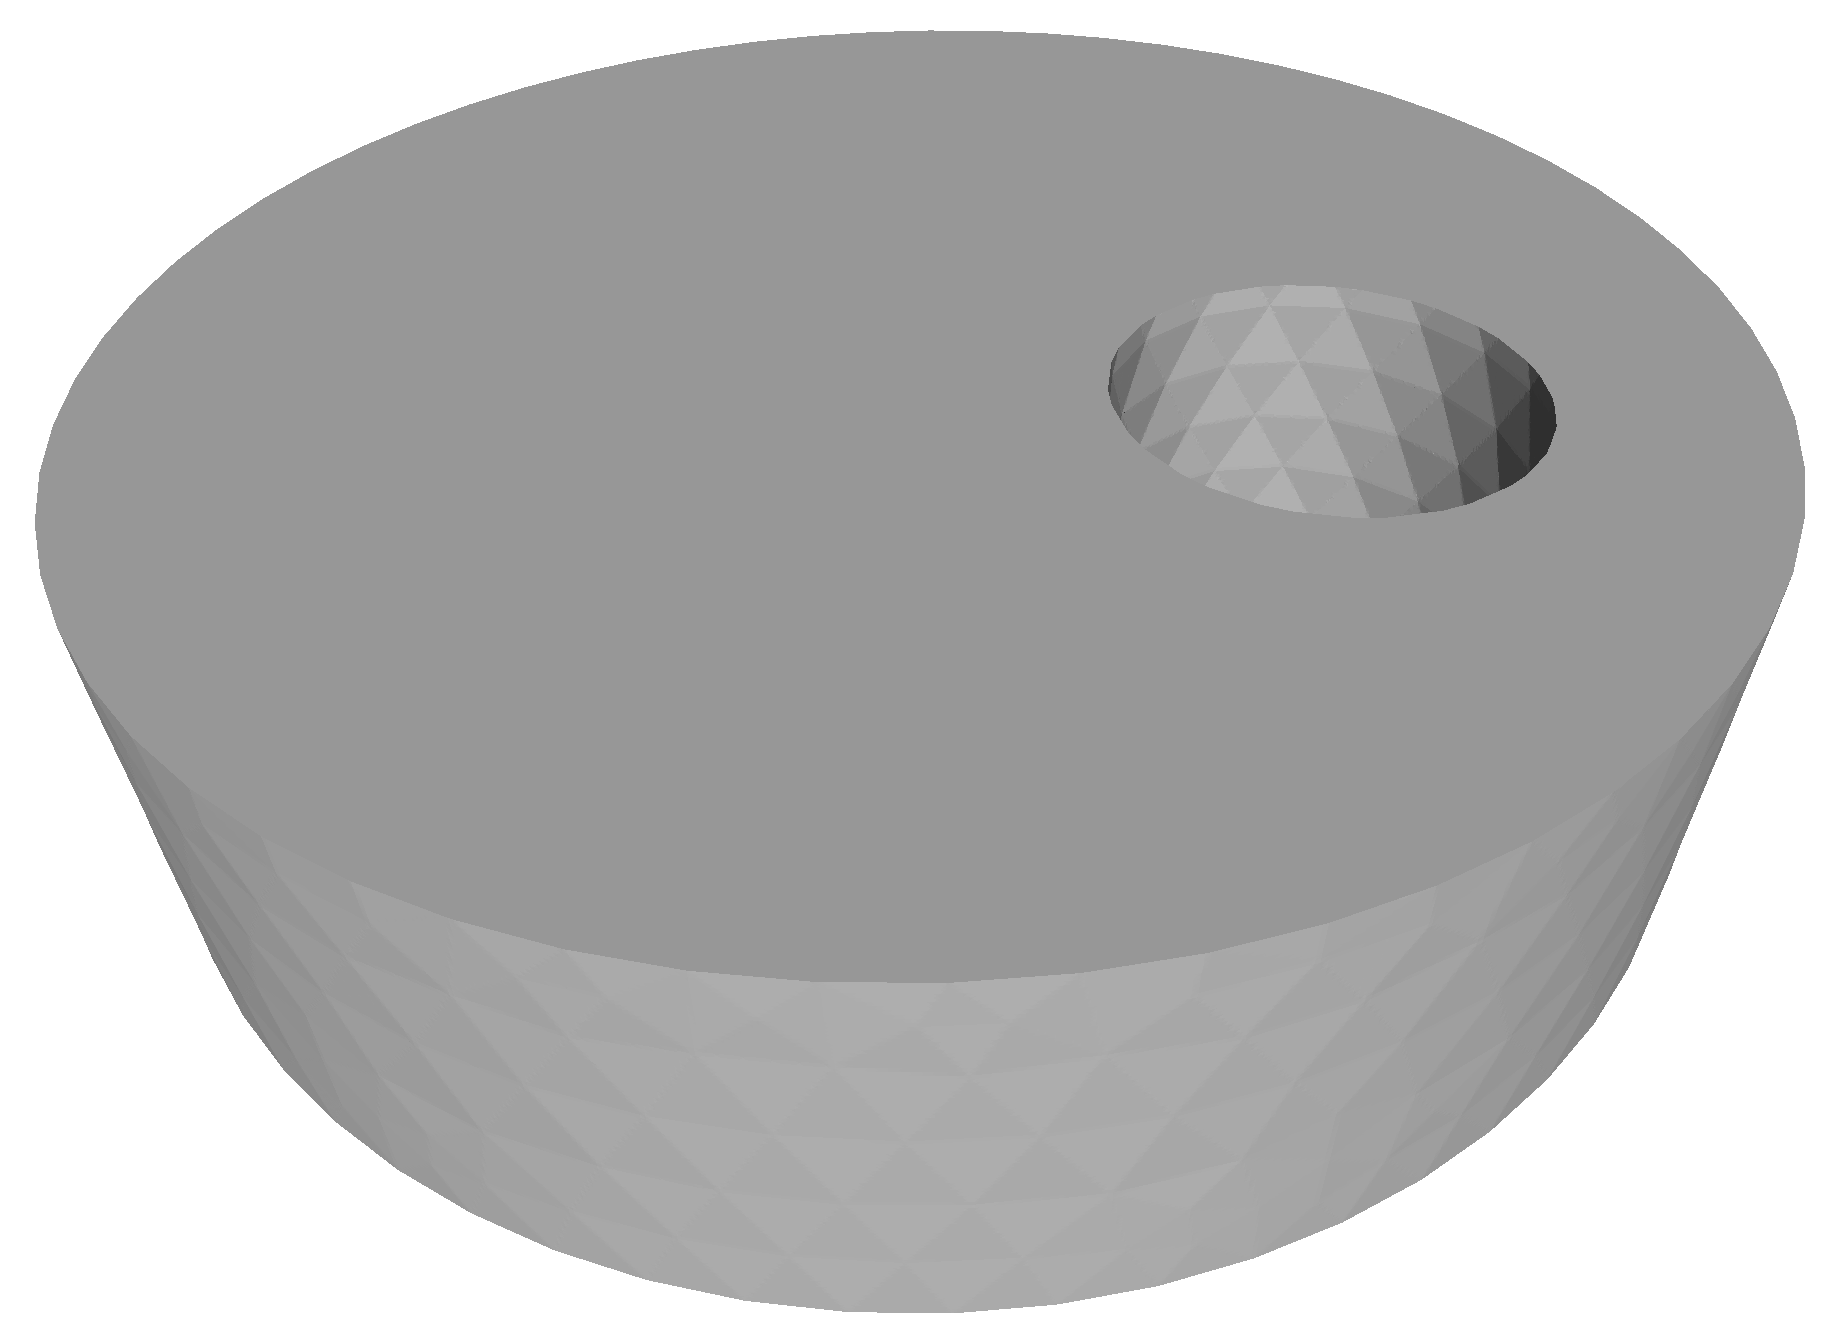
\includegraphics[width=\textwidth]{td_cylinders_d}
		\caption{\cylindersd}
		\label{fig:td_cylinders_delaunay}
	\end{subfigure}
	\begin{subfigure}[b]{0.34\textwidth}
		\centering
		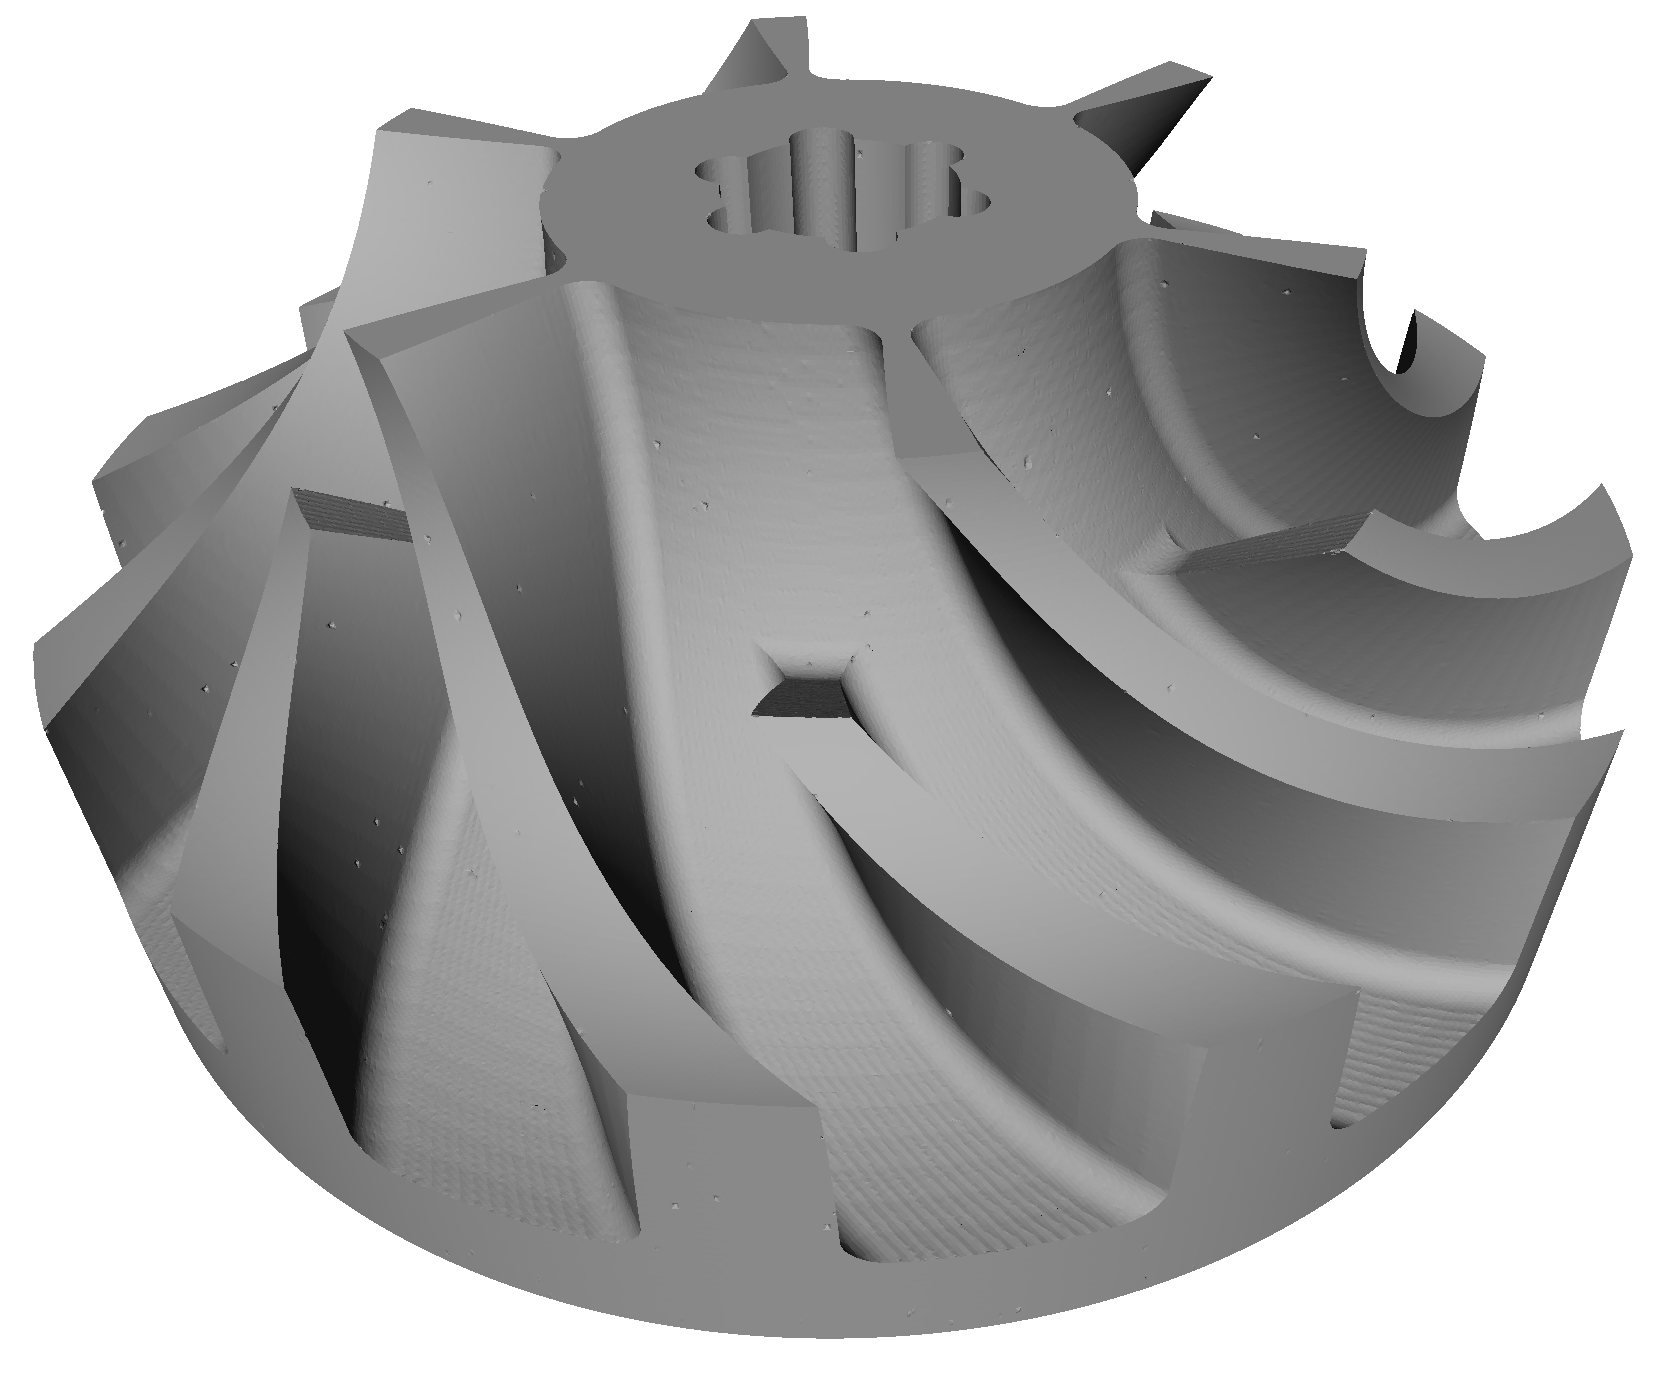
\includegraphics[width=\textwidth]{td_hq_impeller}
		\caption{\impeller}
		\label{fig:td_hq_impeller}
	\end{subfigure}
	\hspace{1cm}
	\begin{subfigure}[b]{0.34\textwidth}
		\centering
		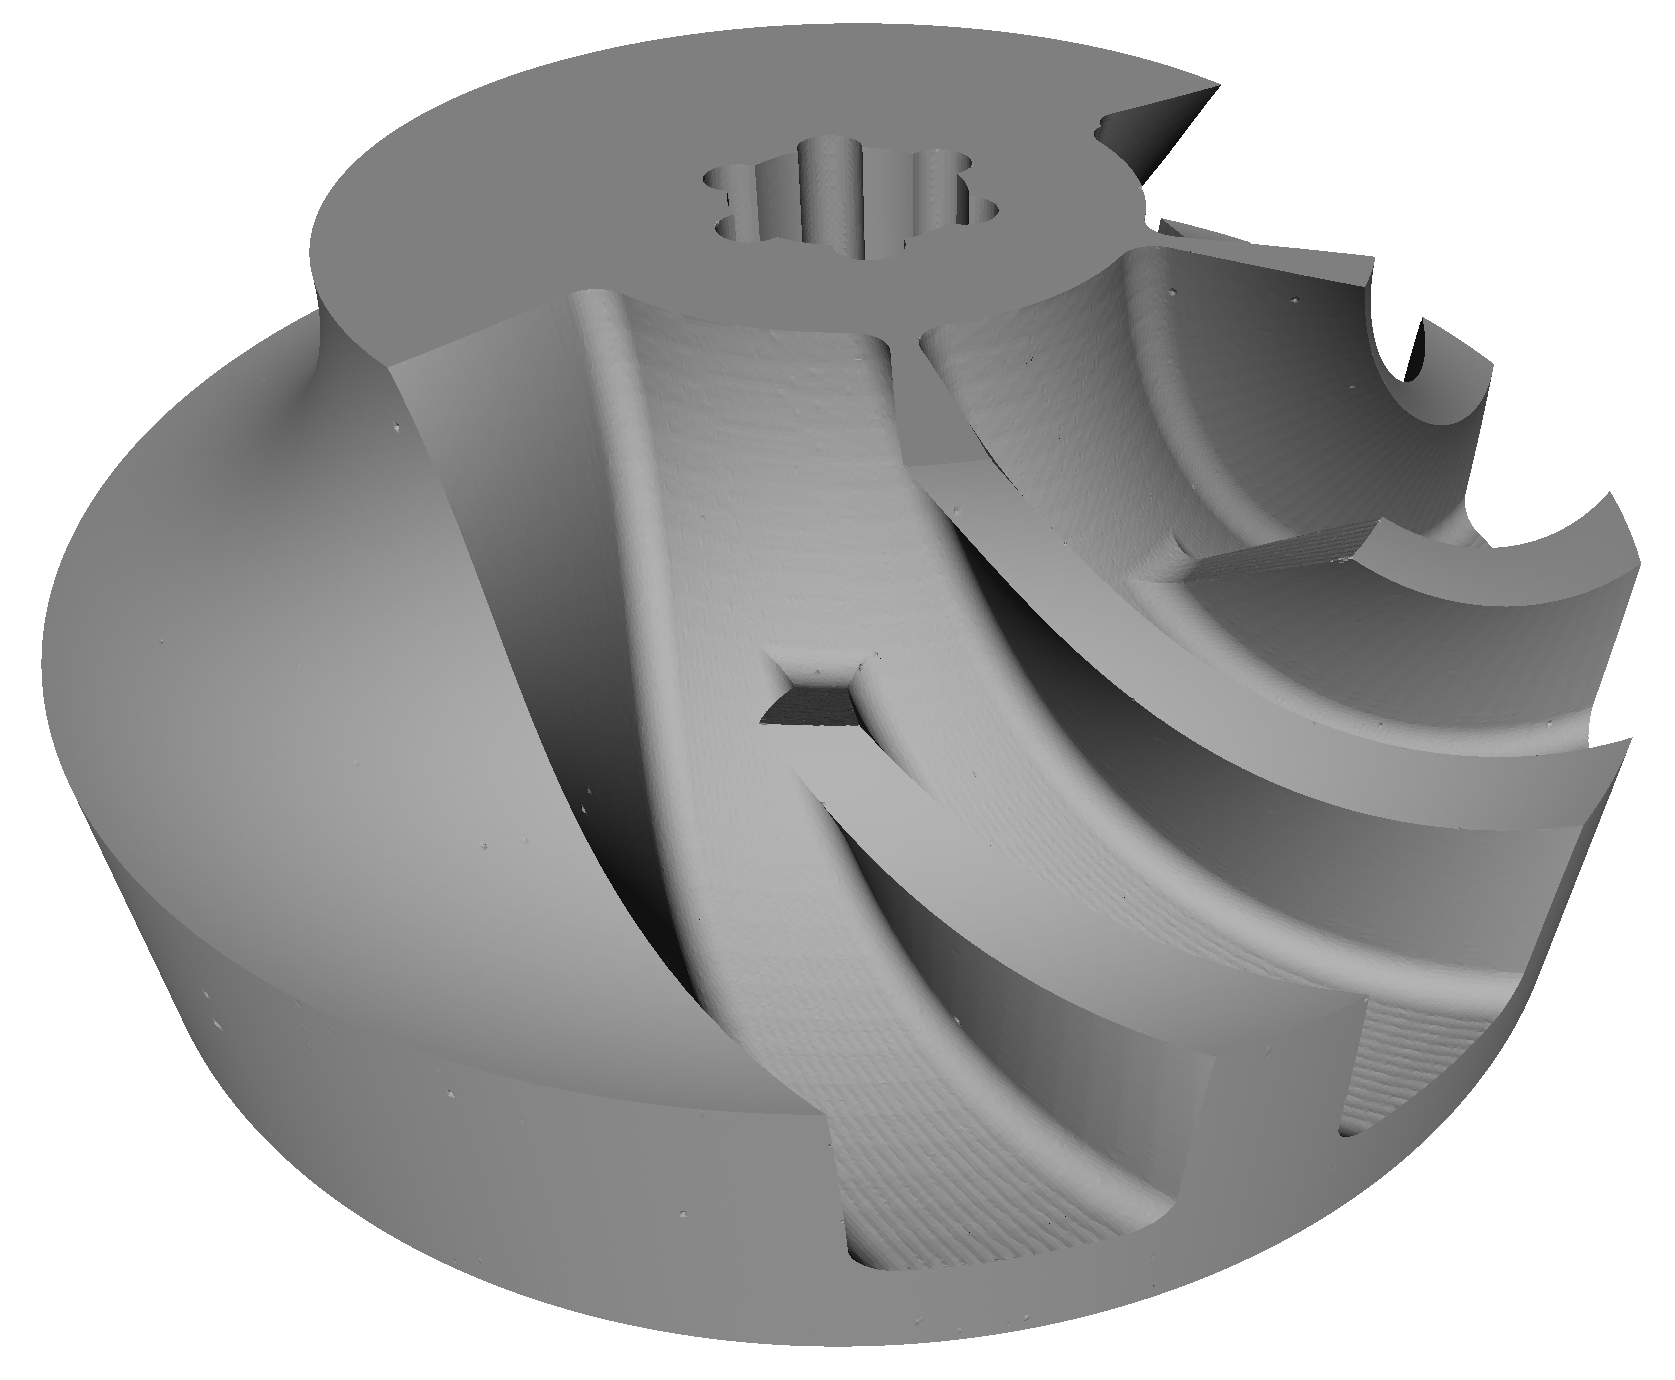
\includegraphics[width=\textwidth]{td_hq_impeller_2}
		\caption{\impellerhalf}
		\label{fig:td_hq_impeller_2}
	\end{subfigure}
	\begin{subfigure}[b]{0.33\textwidth}
		\centering
		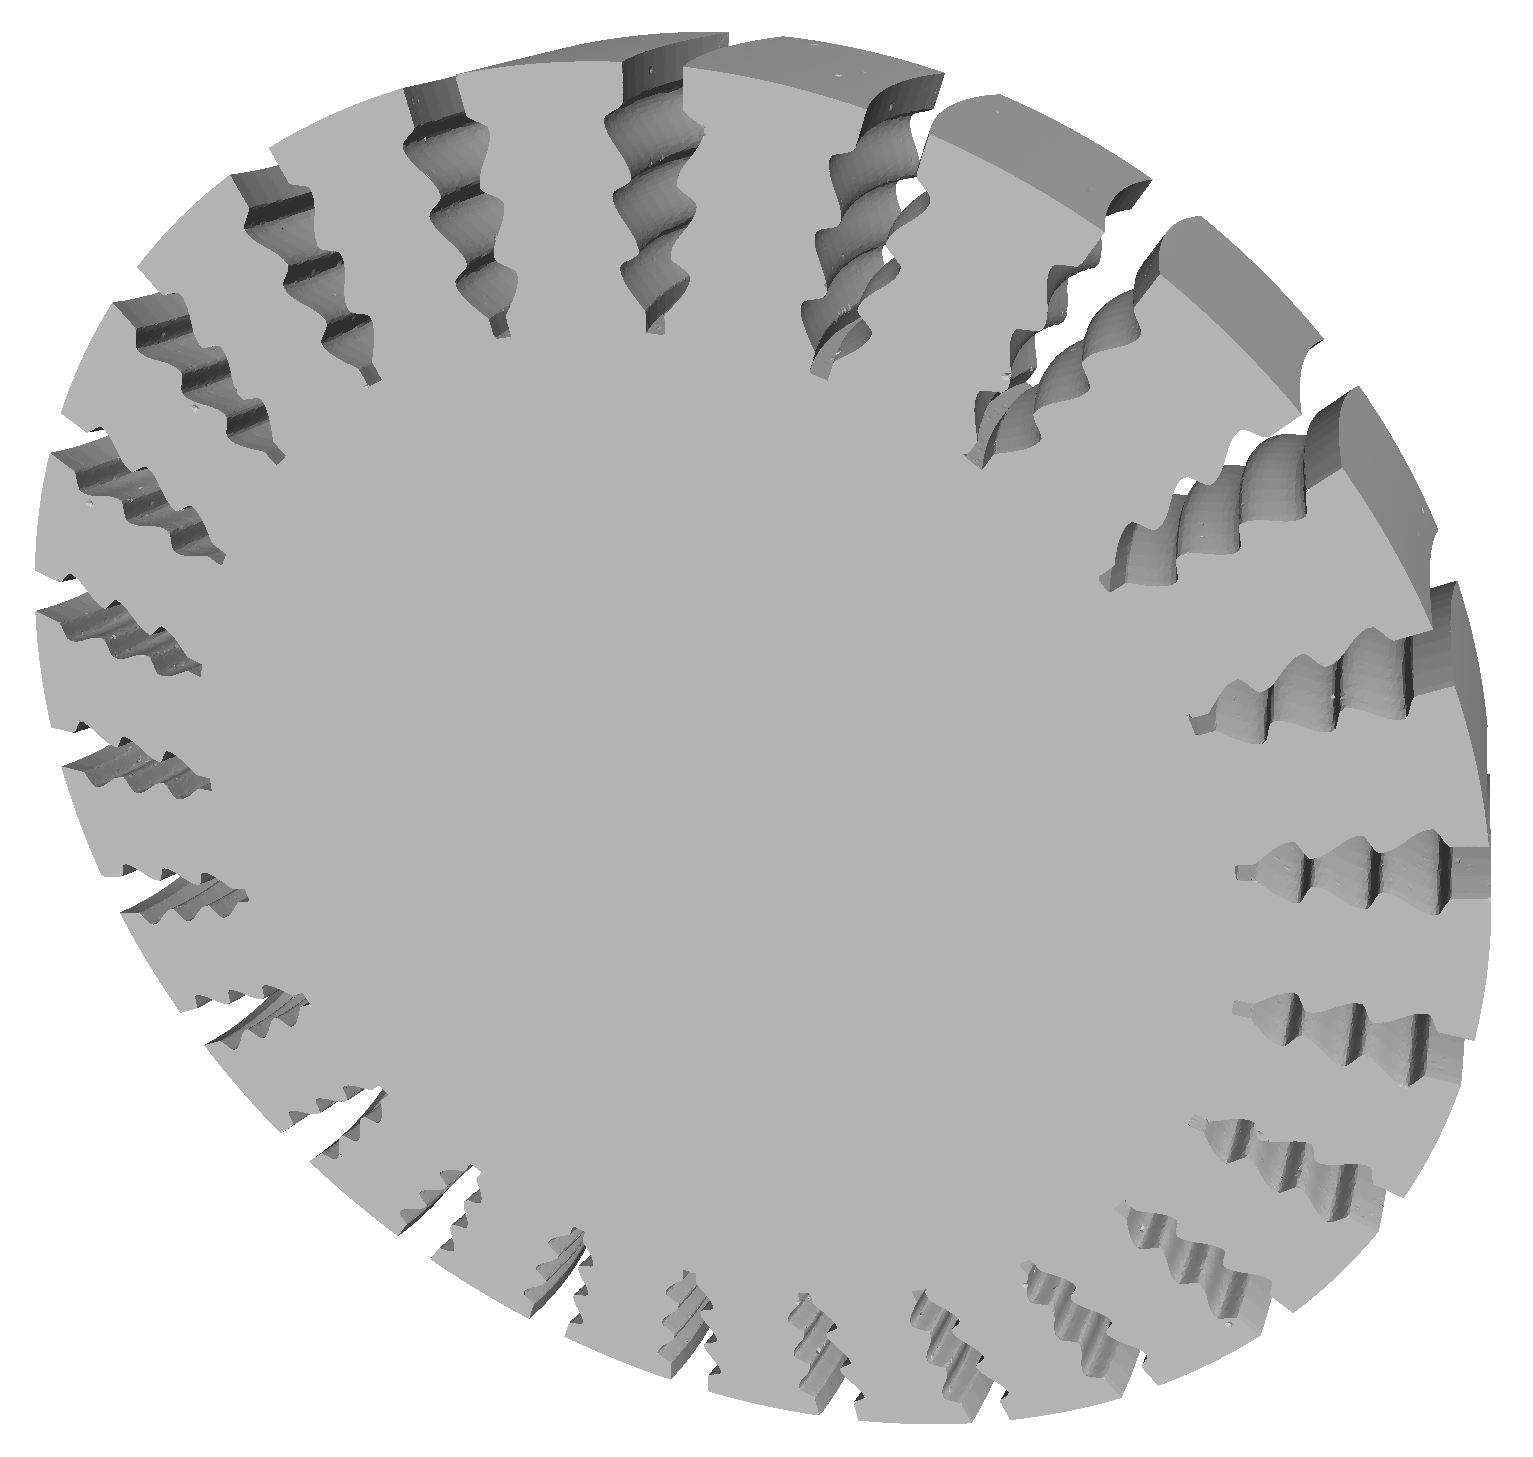
\includegraphics[width=\textwidth]{td_turbine}
		\caption{\turbine}
		\label{fig:td_turbine}
	\end{subfigure}
	\caption[Tri-dexel result renderings]{
		Renderings of the result meshes after applying the tri-dexel reconstruction approach with a grid resolution of 400 on the selected test scenes in \cref{tbl:test_scenes}.
	}
	\label{fig:td_results}
\end{figure}

\Cref{fig:td_hq_impeller_details} shows two detailed renderings of the \impeller scene.

\begin{figure}
	\centering
	\begin{subfigure}[b]{0.49\textwidth}
		\centering
		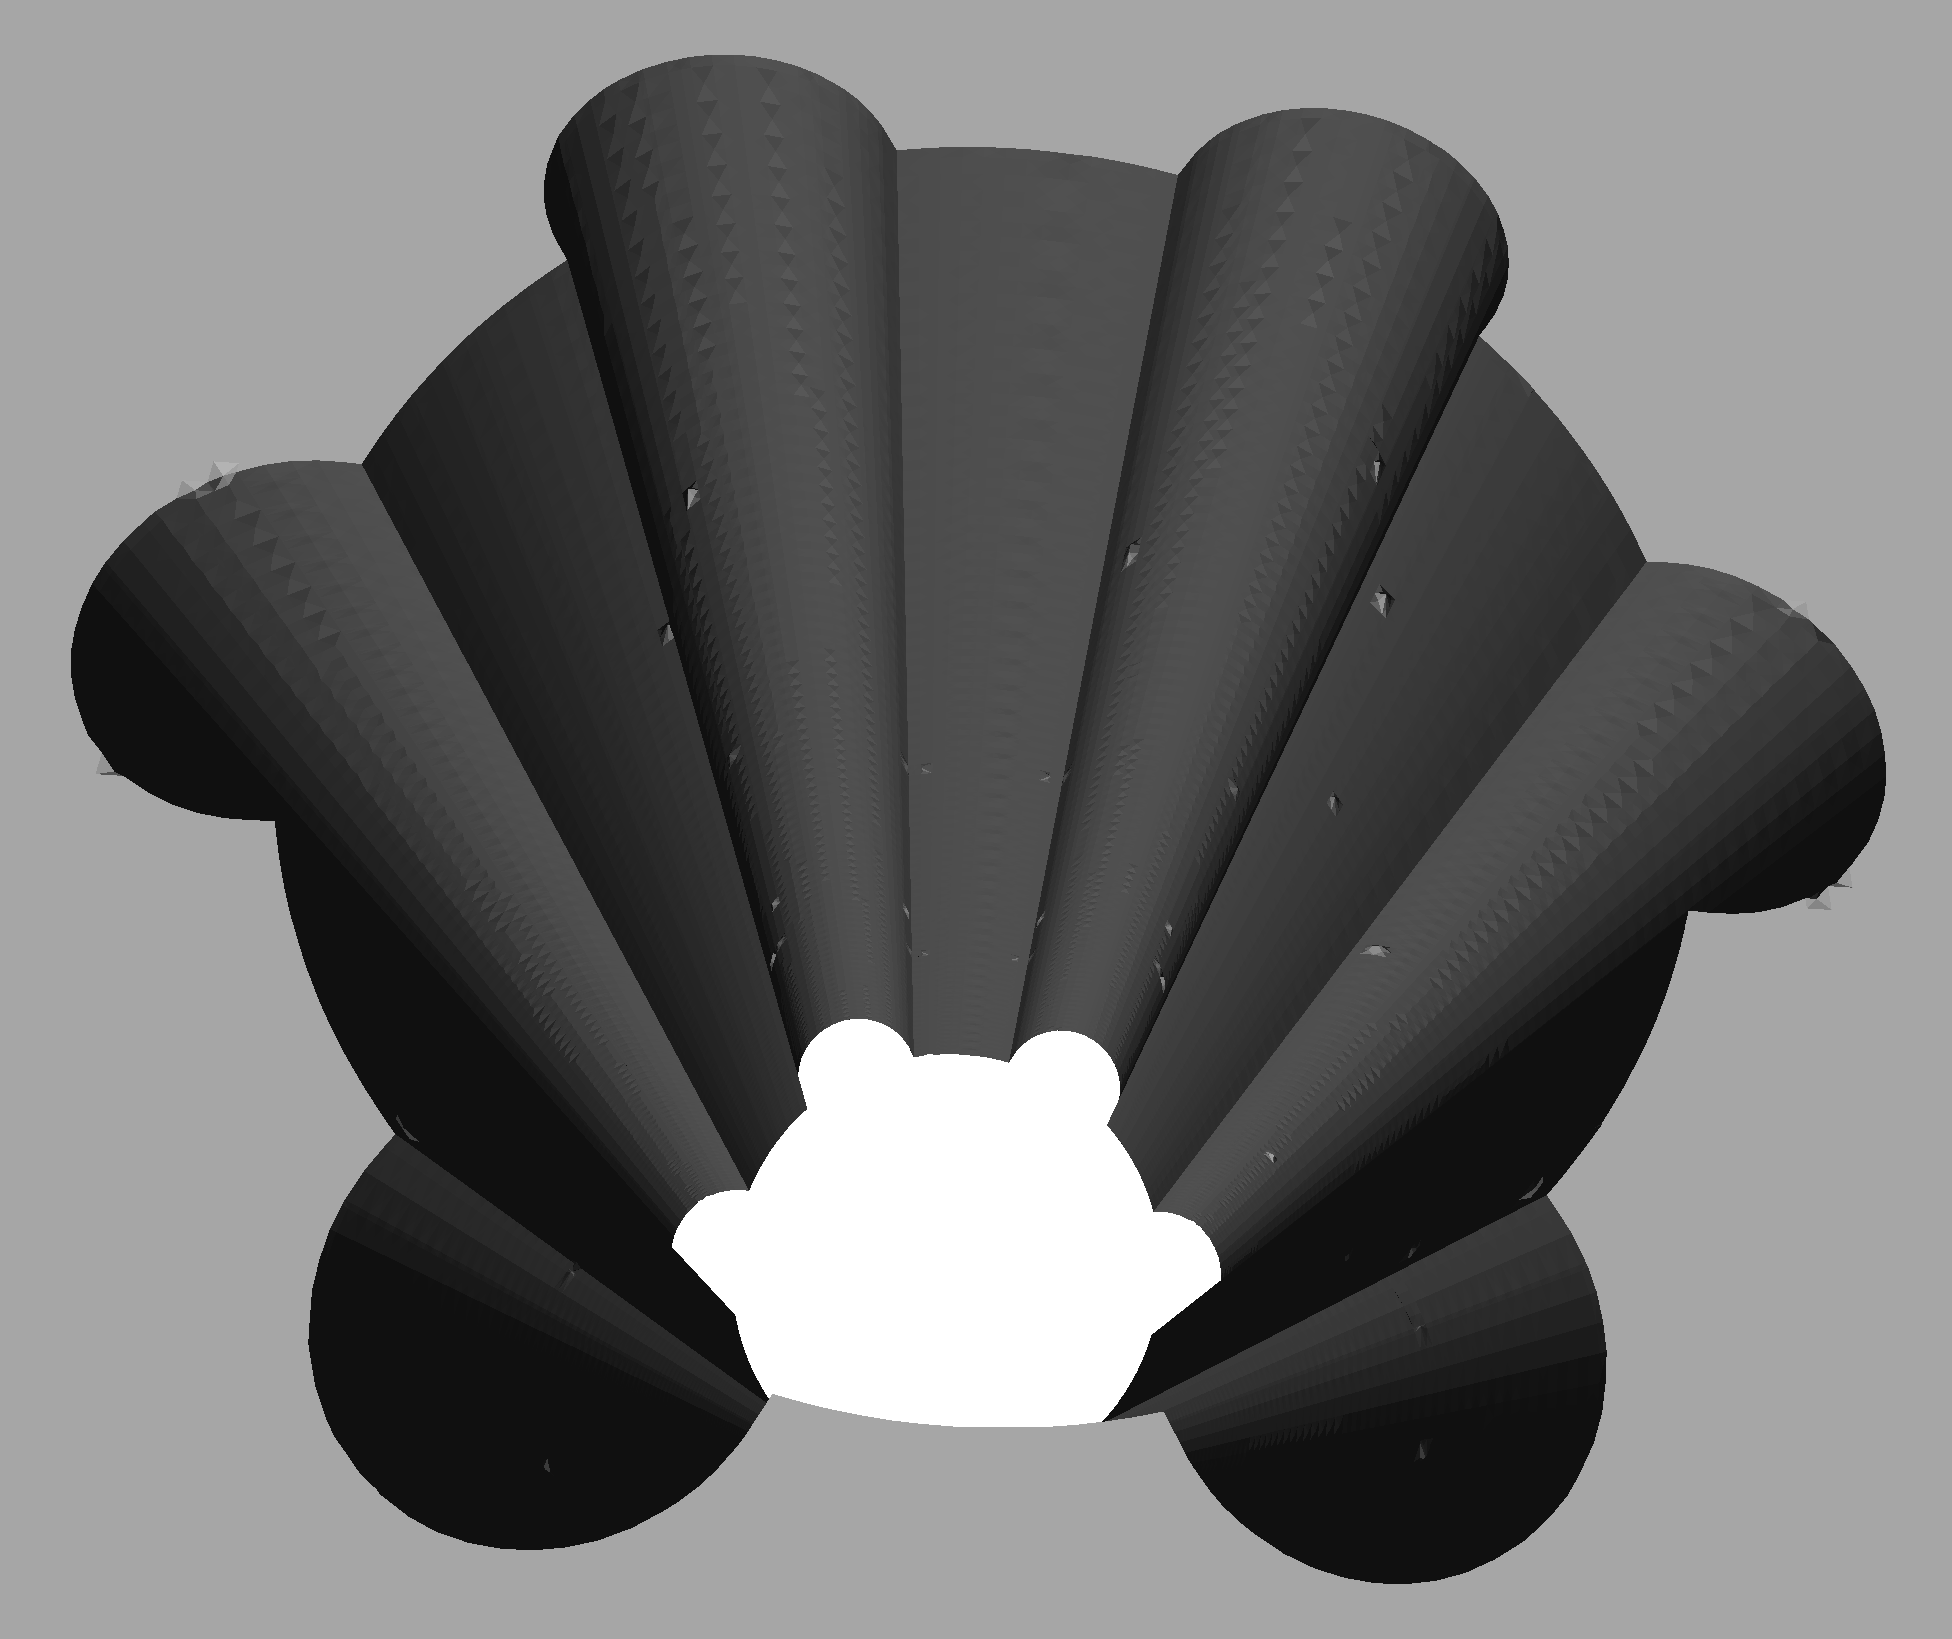
\includegraphics[width=\textwidth]{td_hq_impeller_drillings}
		\caption{\impeller drillings}
		\label{fig:td_hq_impeller_drillings}
	\end{subfigure}
	\begin{subfigure}[b]{0.49\textwidth}
		\centering
		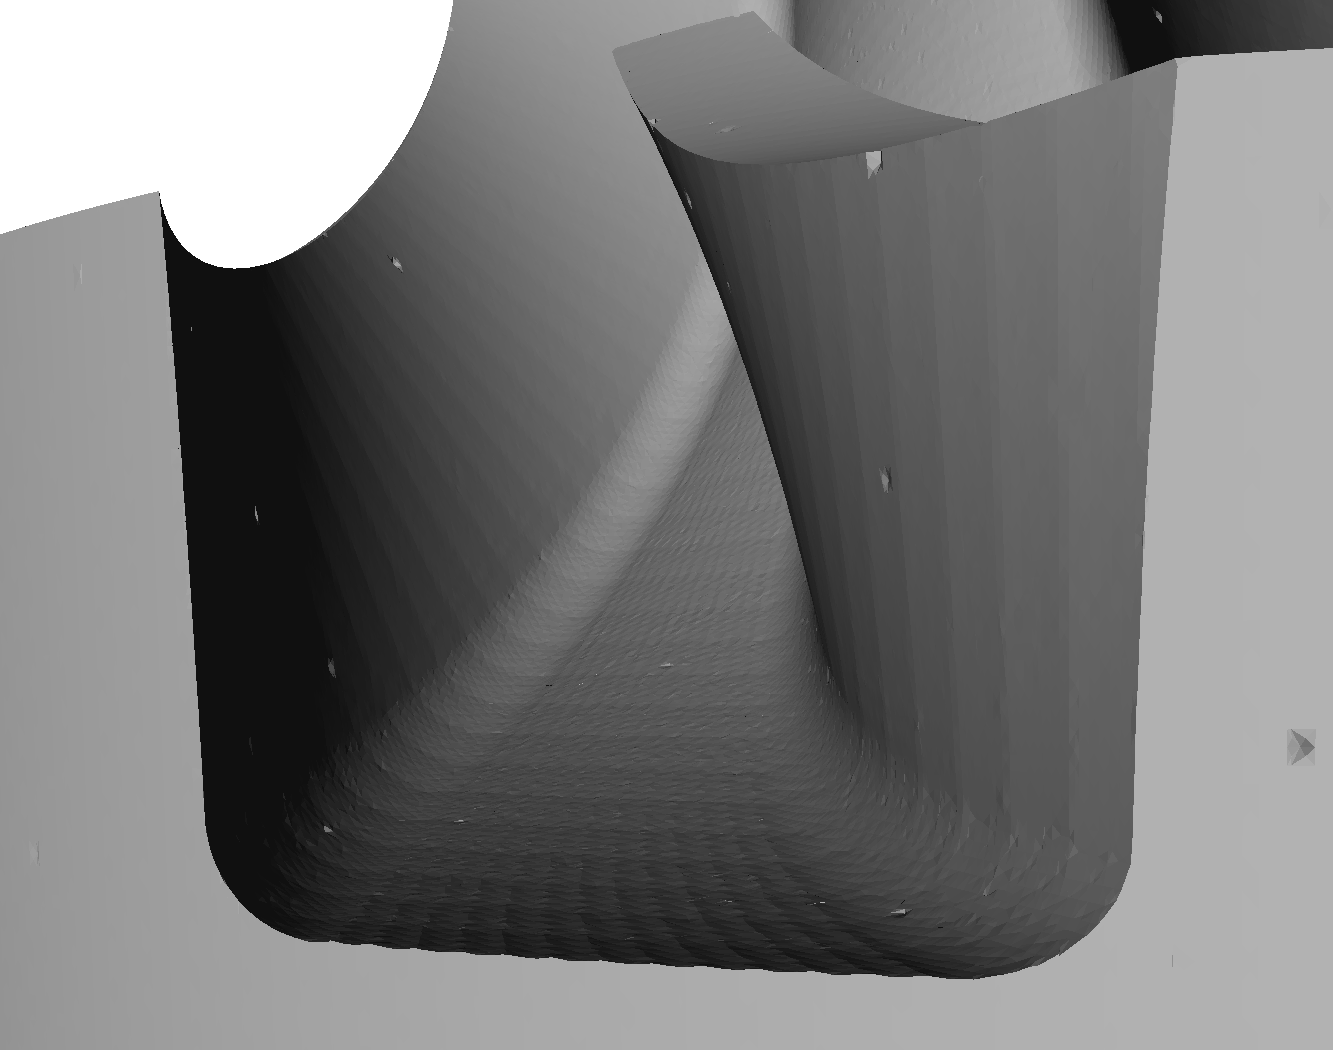
\includegraphics[width=\textwidth]{td_hq_impeller_blades}
		\caption{\impeller blades}
		\label{fig:td_hq_impeller_blades}
	\end{subfigure}
	\caption[Tri-dexel result details]{
		Details of the \impeller scene extracted using the tri-dexel approach with a grid resolution of 400.
	}
	\label{fig:td_hq_impeller_details}
\end{figure}

\Cref{fig:td_grooves} shows renderings of a detailed view on one of the grooves in different resolutions.

\begin{figure}
	\centering
	\begin{subfigure}[b]{0.24\textwidth}
		\centering
		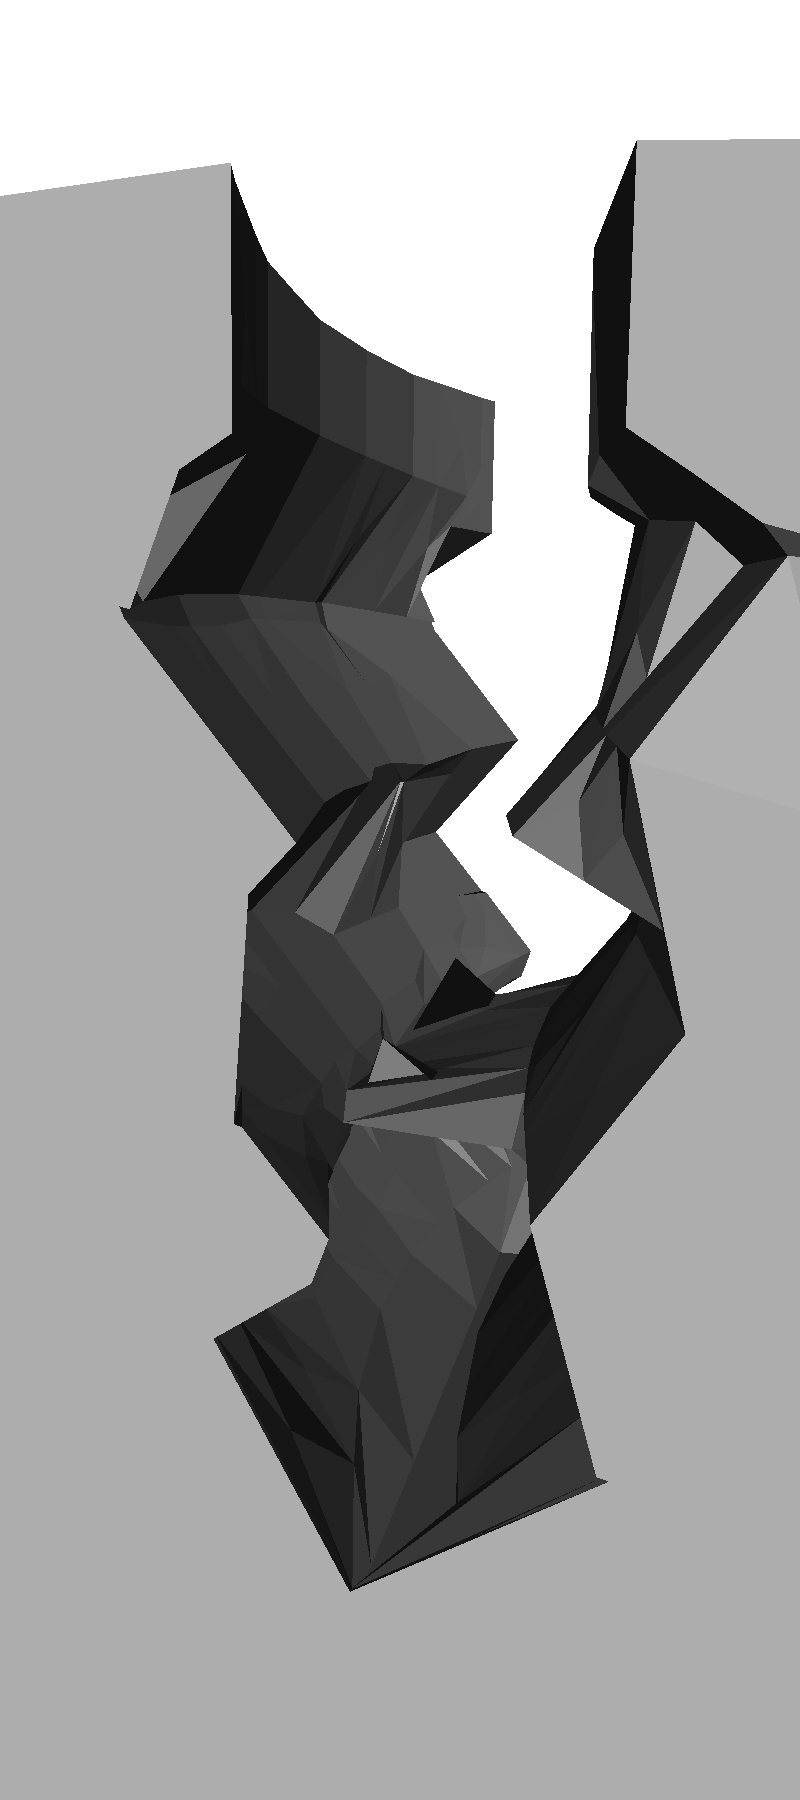
\includegraphics[width=\textwidth]{td_turbine_groove_50}
		\caption{50}
		\label{fig:td_turbine_groove_50}
	\end{subfigure}
	\begin{subfigure}[b]{0.24\textwidth}
		\centering
		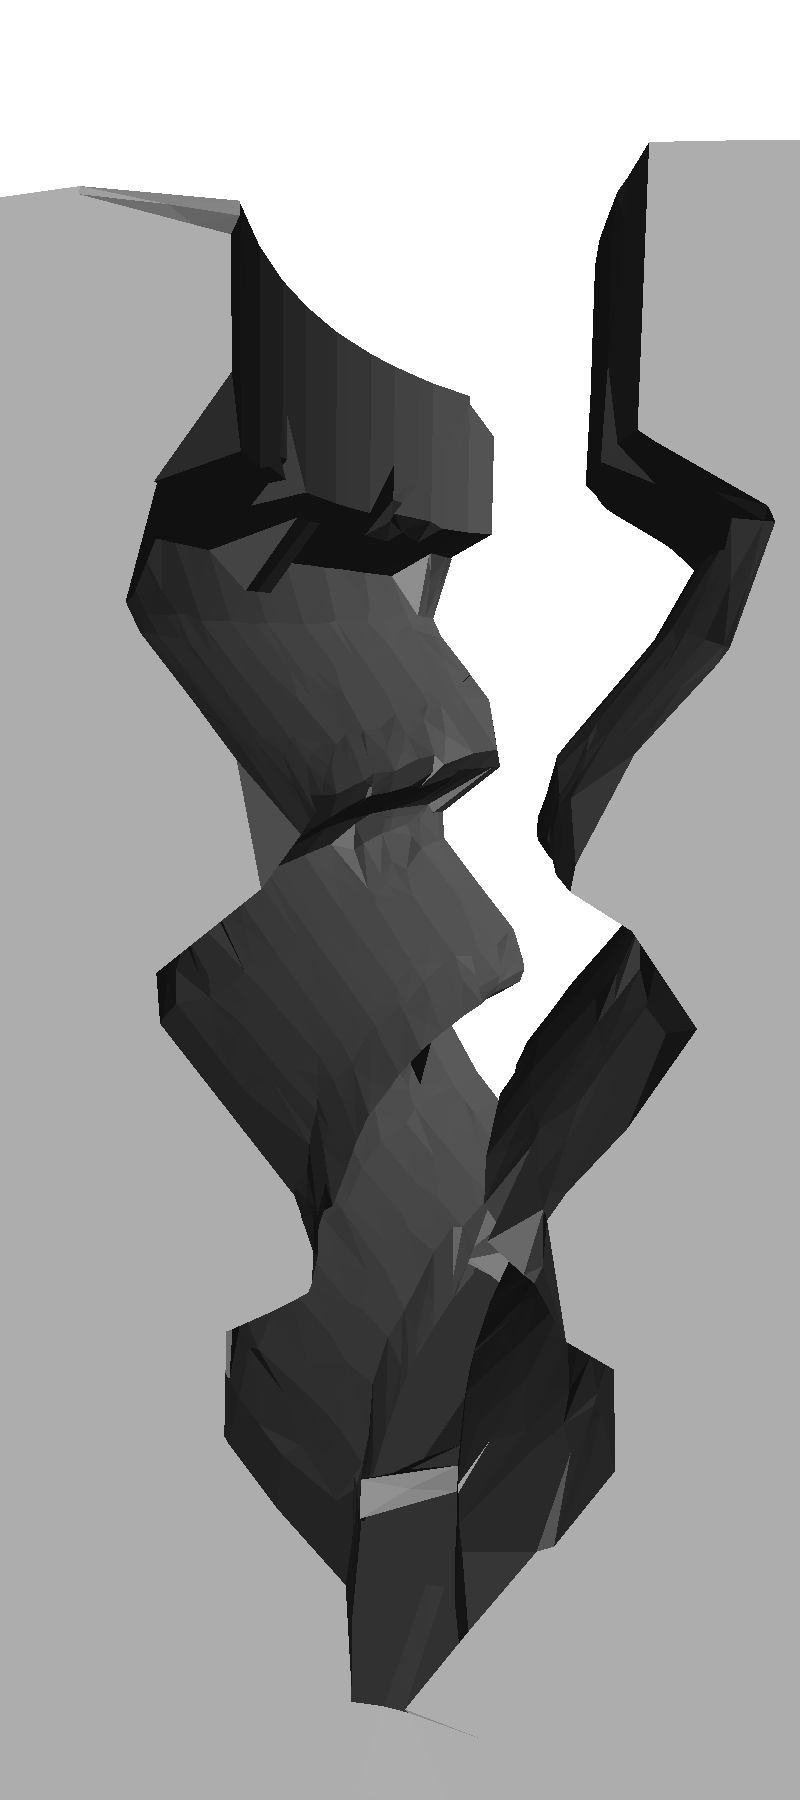
\includegraphics[width=\textwidth]{td_turbine_groove_100}
		\caption{100}
		\label{fig:td_turbine_groove_100}
	\end{subfigure}
	\begin{subfigure}[b]{0.24\textwidth}
		\centering
		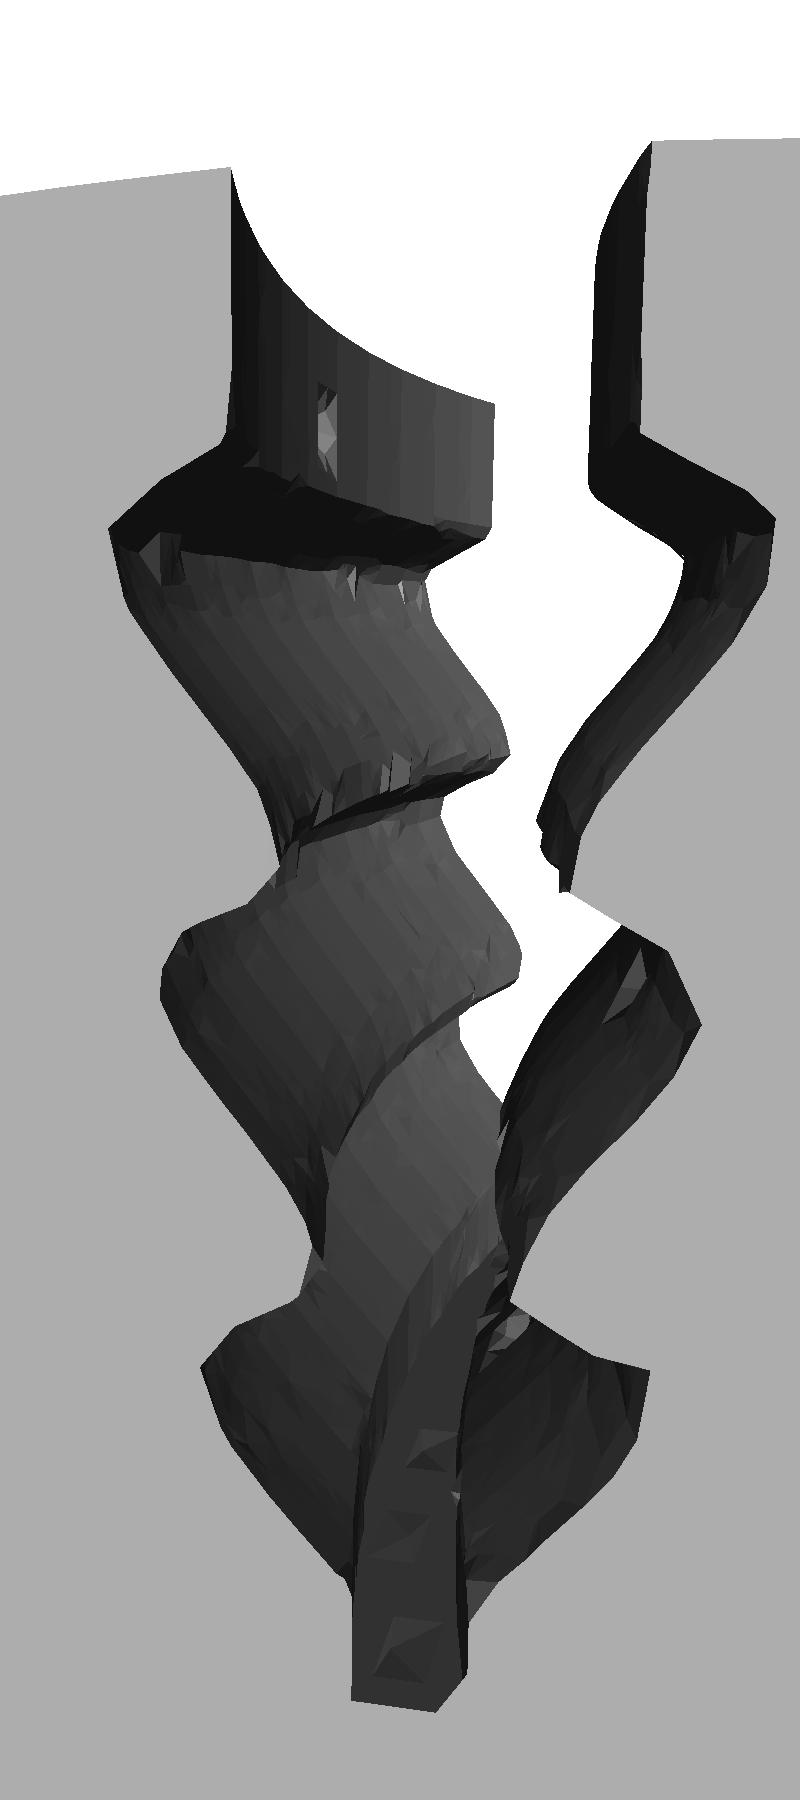
\includegraphics[width=\textwidth]{td_turbine_groove_200}
		\caption{200}
		\label{fig:td_turbine_groove_200}
	\end{subfigure}
	\begin{subfigure}[b]{0.24\textwidth}
		\centering
		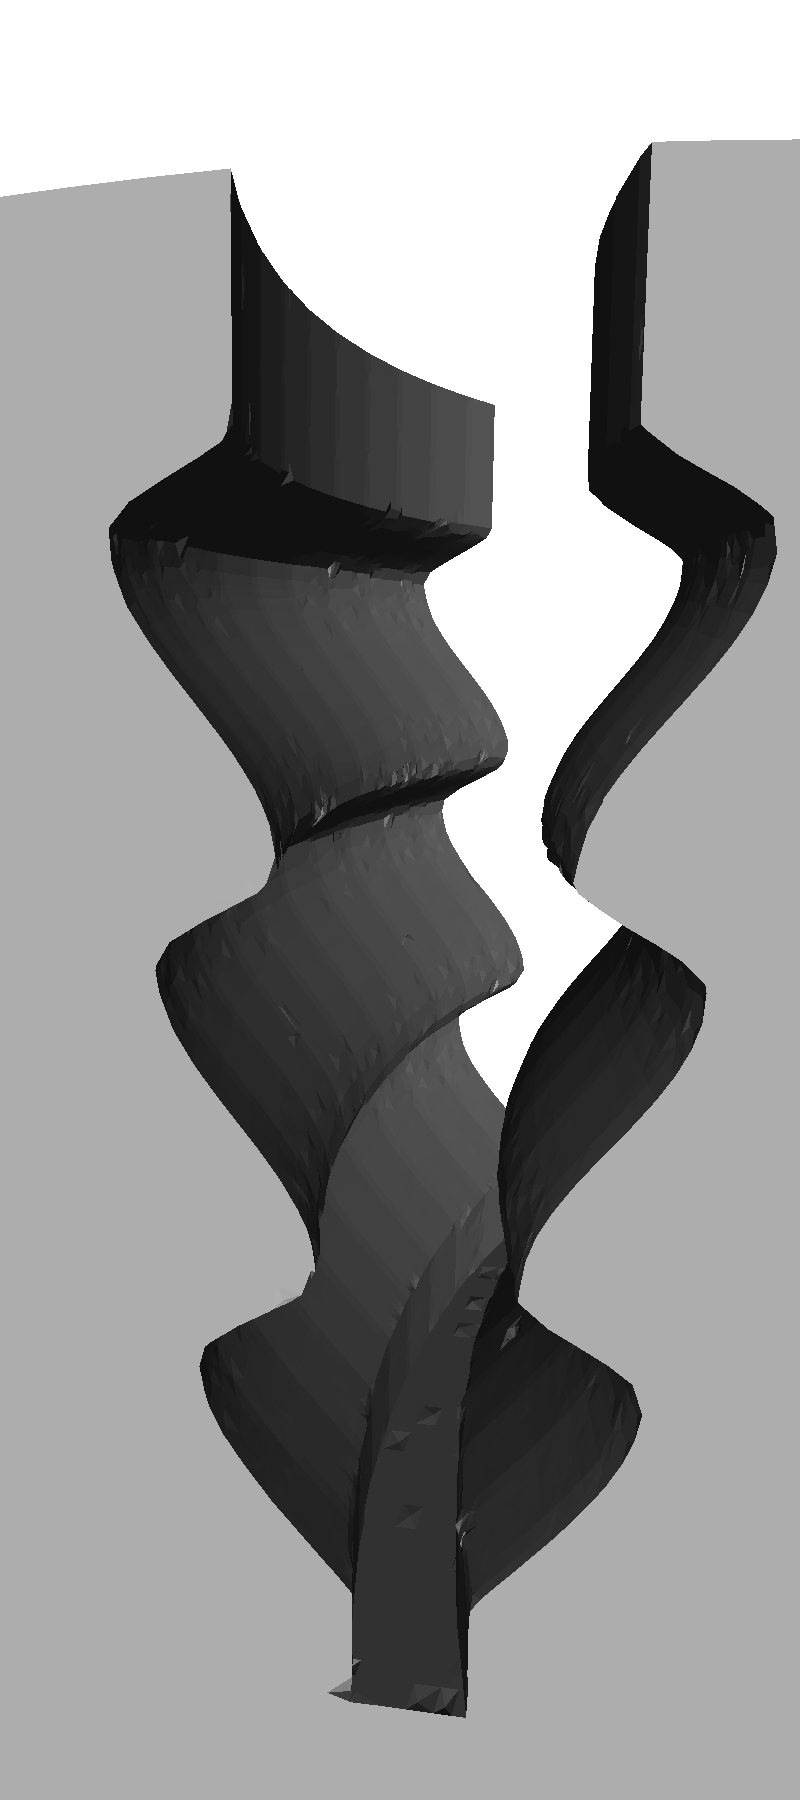
\includegraphics[width=\textwidth]{td_turbine_groove_400}
		\caption{400}
		\label{fig:td_turbine_groove_400}
	\end{subfigure}
	\caption[Tri-dexel \turbine grooves]{
		Detailed renderings with the same perspective of a groove of the \turbine scene.
		The meshes were created using the tri-dexel reconstruction algorithm with the grid resolutions 50, 100, 200 and 400.
	}
	\label{fig:td_grooves}
\end{figure}

\Cref{fig:td_features_and_cell_slicing} shows the different outcome when using no refinement/feature reconstruction, using feature reconstruction and using feature reconstruction and cell slicing.

\begin{figure}
	\centering
	\begin{subfigure}[b]{0.67\textwidth}
		\centering
		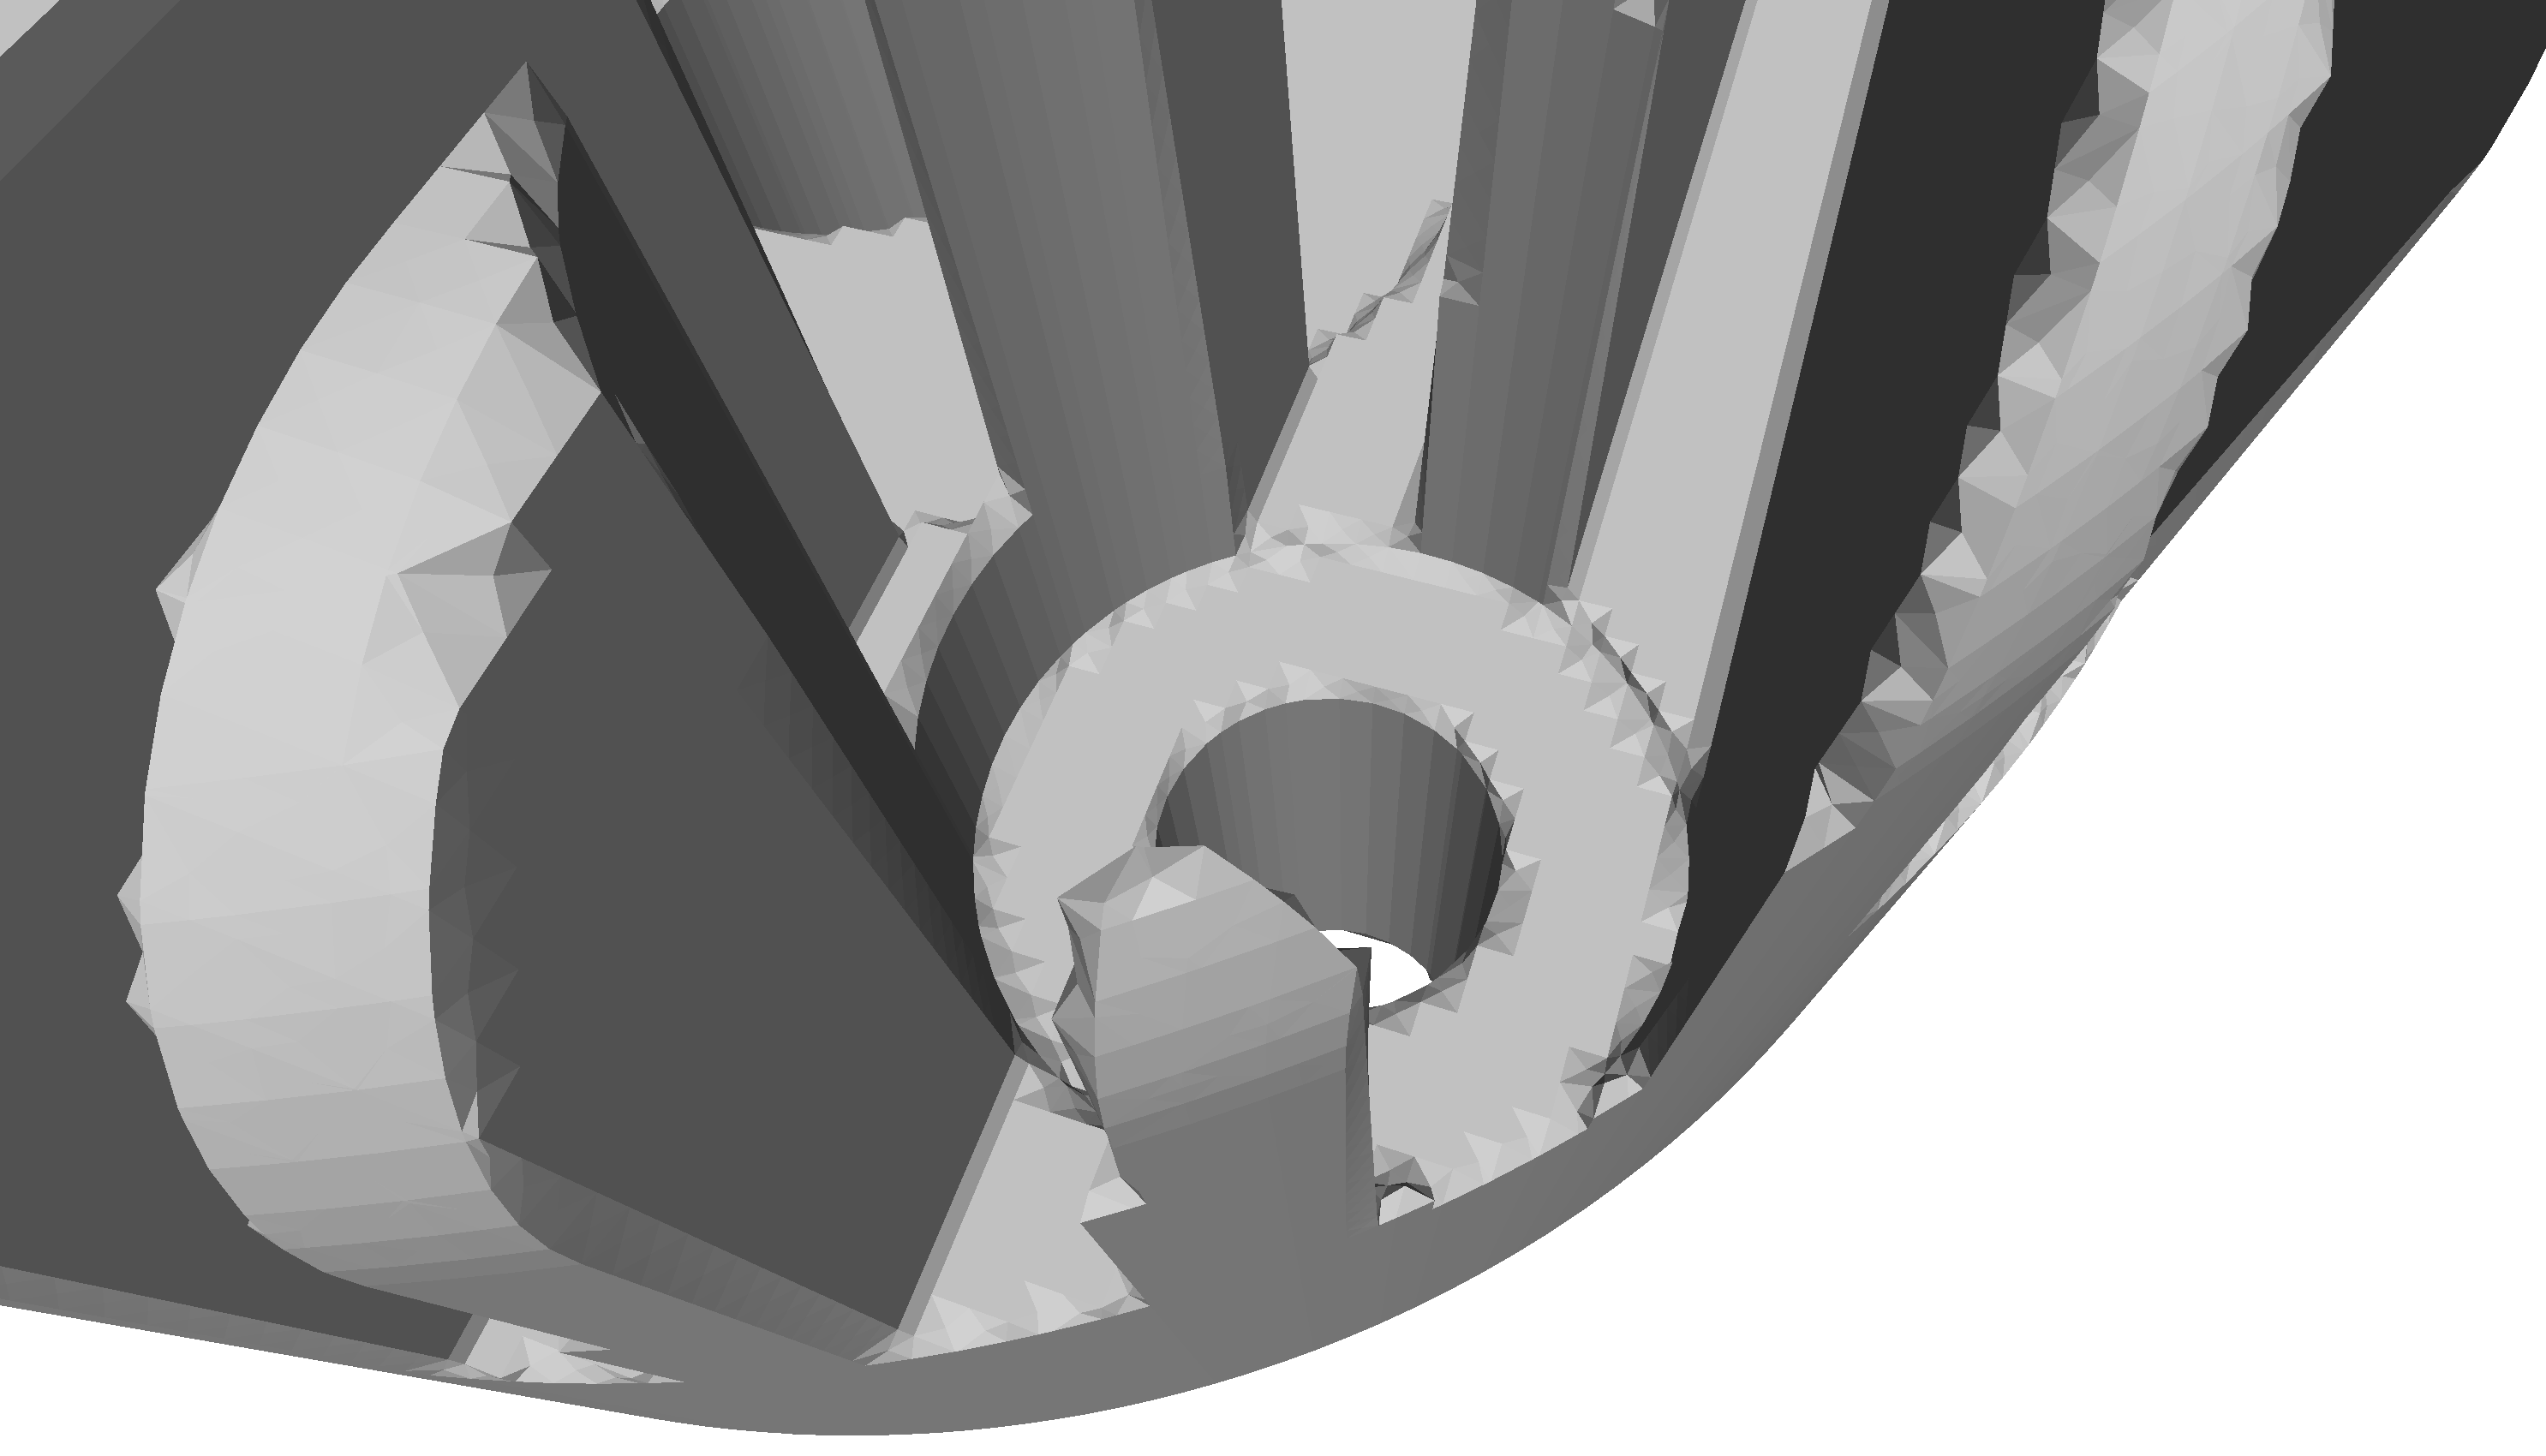
\includegraphics[width=\textwidth]{td_cylinder_head_drilling_no_features}
		\caption{no feature reconstruction}
		\label{fig:td_cylinder_head_drilling_no_features}
	\end{subfigure}
	\bigskip\\
	\begin{subfigure}[b]{0.67\textwidth}
		\centering
		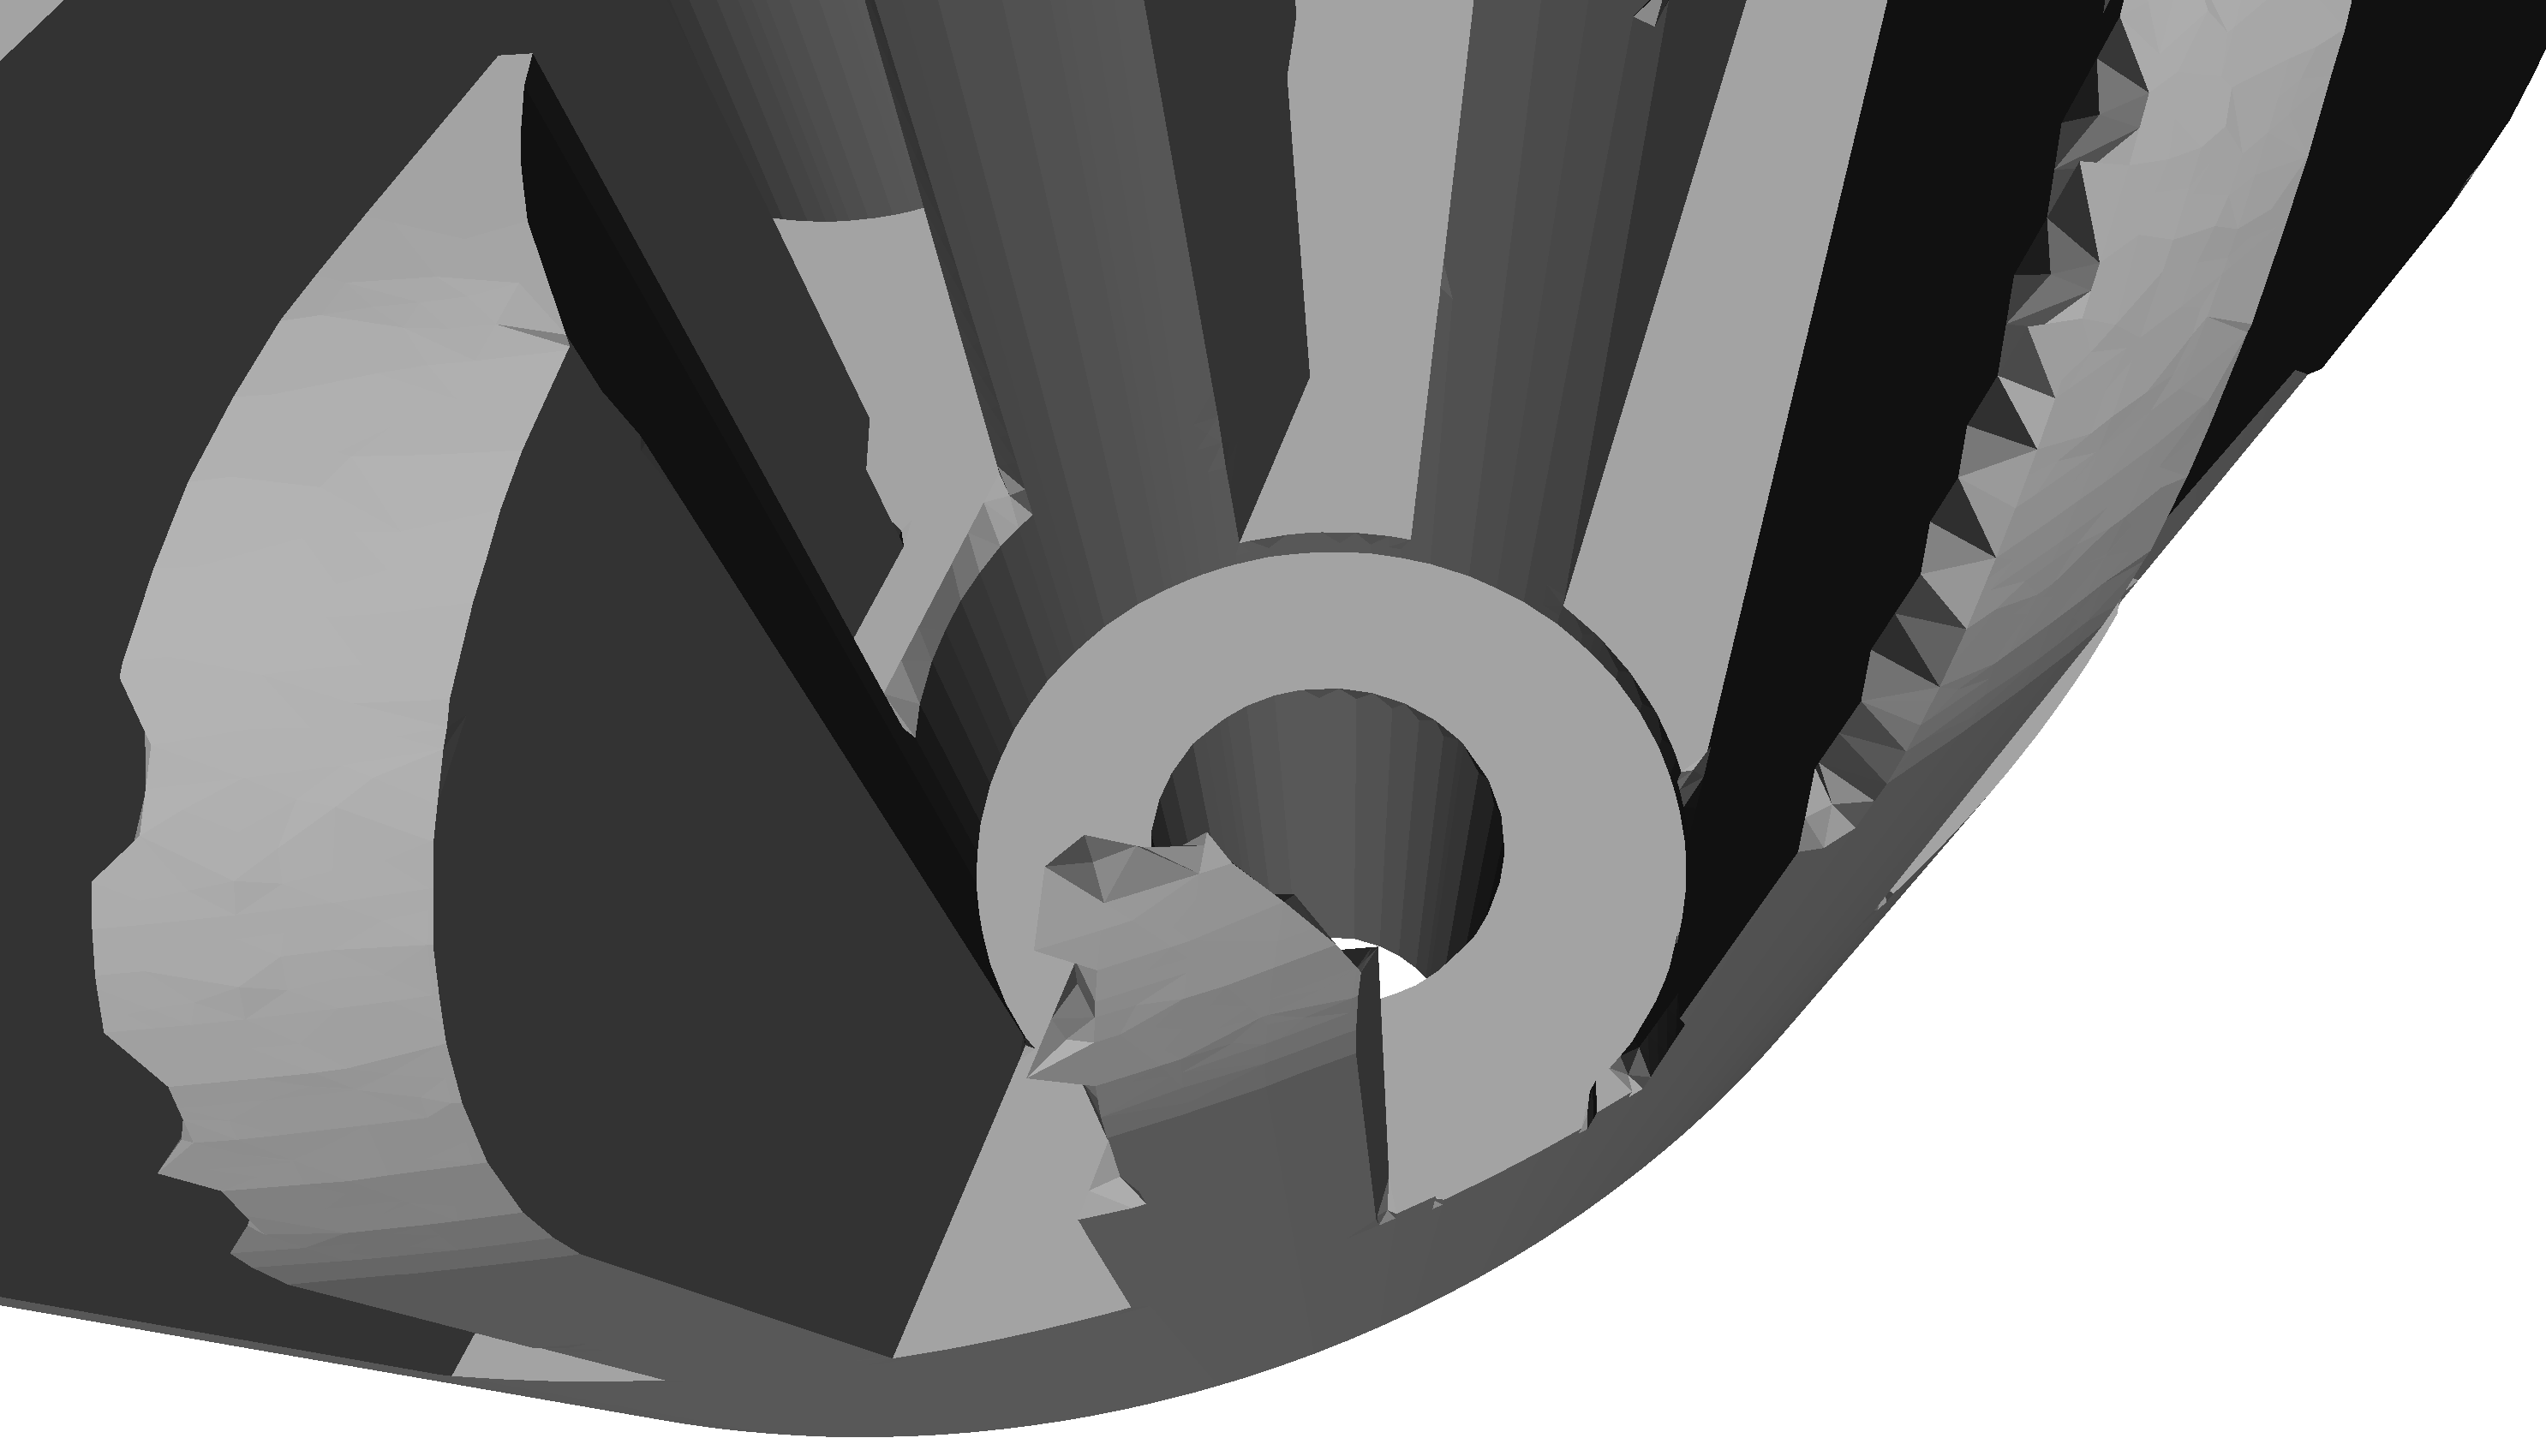
\includegraphics[width=\textwidth]{td_cylinder_head_drilling_features}
		\caption{feature reconstruction}
		\label{fig:td_cylinder_head_drilling_features}
	\end{subfigure}
	\bigskip\\
	\begin{subfigure}[b]{0.67\textwidth}
		\centering
		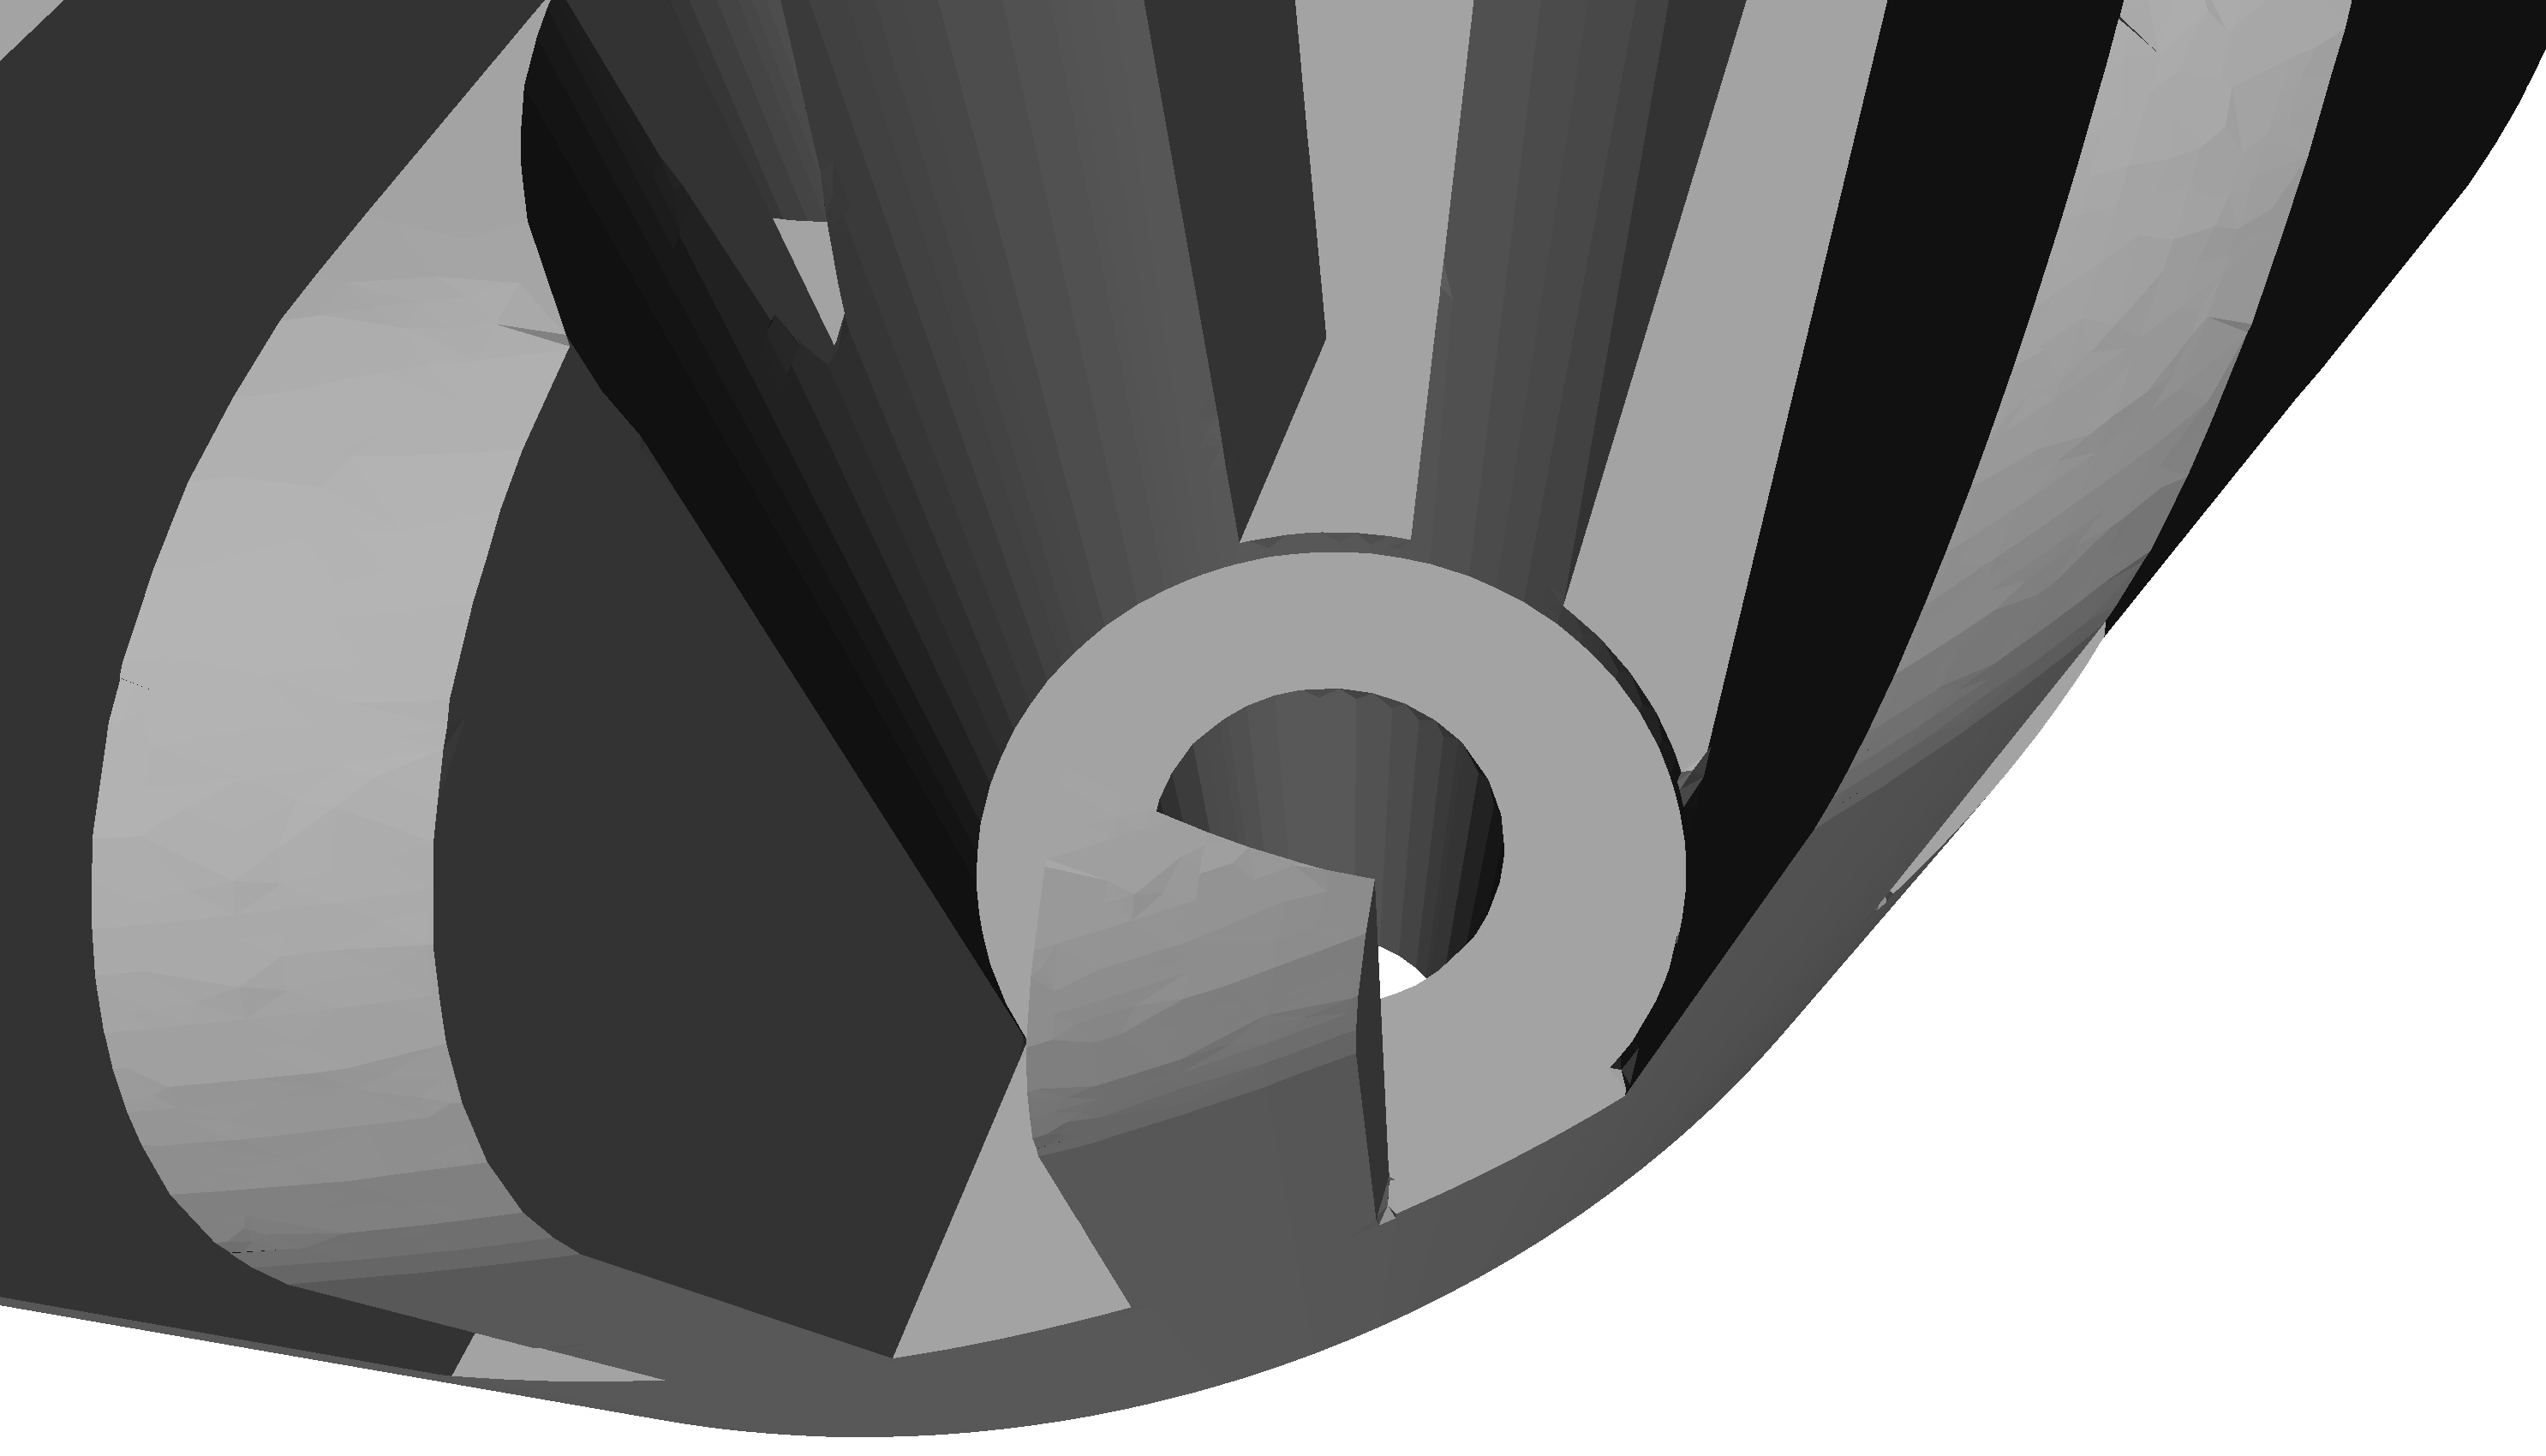
\includegraphics[width=\textwidth]{td_cylinder_head_drilling_cell_slicing}
		\caption{feature reconstruction and cell slicing}
		\label{fig:td_cylinder_head_drilling_cell_slicing}
	\end{subfigure}
	\caption[Tri-dexel feature reconstruction and cell slicing]{
		Details of the \cylinderhead scene rendered with the same perspective.
		The renderings show the effects of refinement, feature reconstruction and cell slicing.
		The meshes have been extracted using the tri-dexel approach at a grid resolution of 100.
	}
	\label{fig:td_features_and_cell_slicing}
\end{figure}

\Cref{fig:td_cylinder_head_issues} shows cell slicing issues of the outmost rip of the \cylinderhead.

\begin{figure}
	\centering
	\begin{subfigure}[b]{0.49\textwidth}
		\centering
		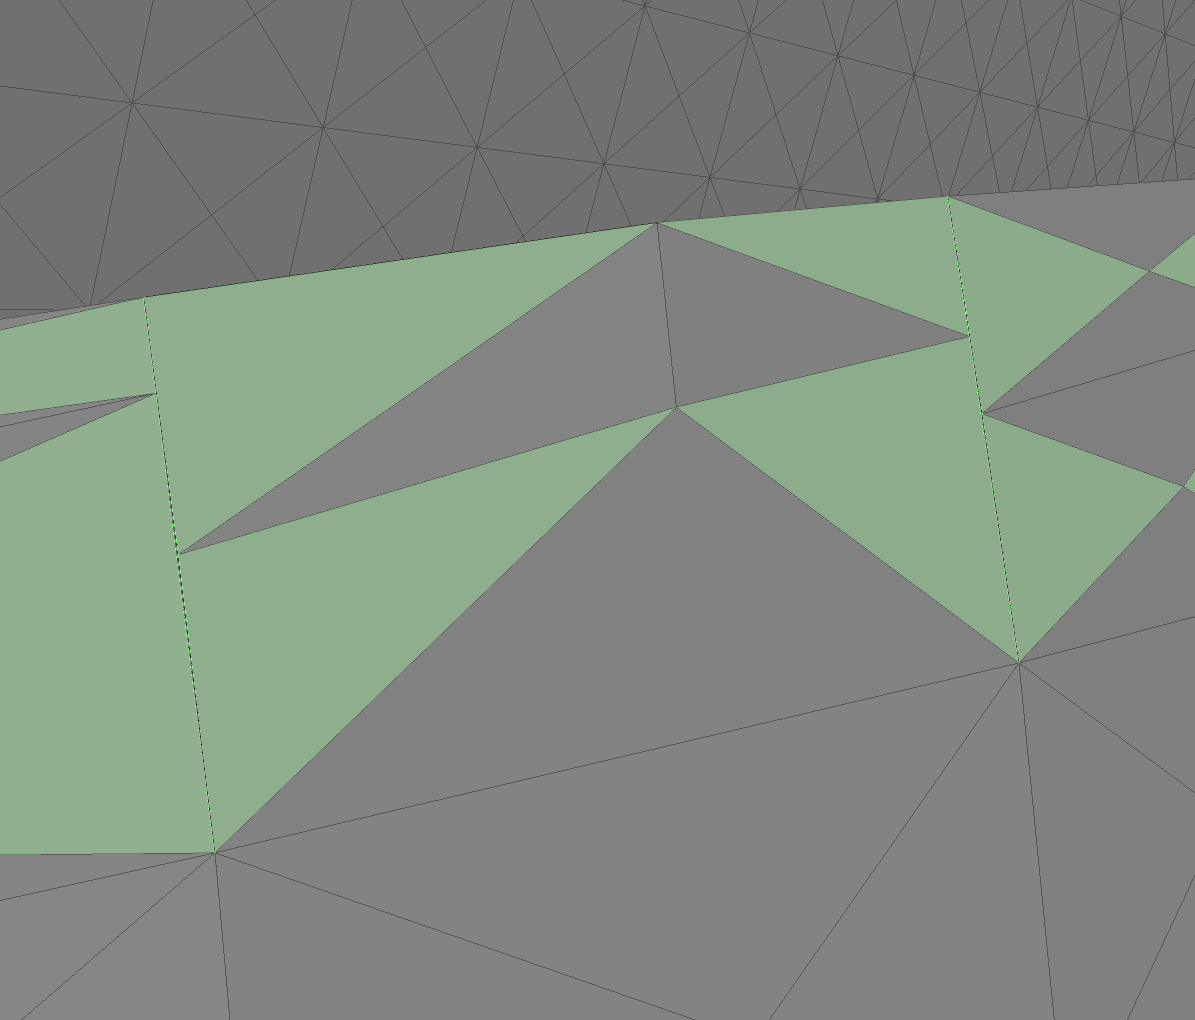
\includegraphics[width=\textwidth]{td_cylinder_head_t_vertex}
		\caption{t-vertices}
		\label{fig:td_cylinder_head_t_vertex}
	\end{subfigure}
	\begin{subfigure}[b]{0.49\textwidth}
		\centering
		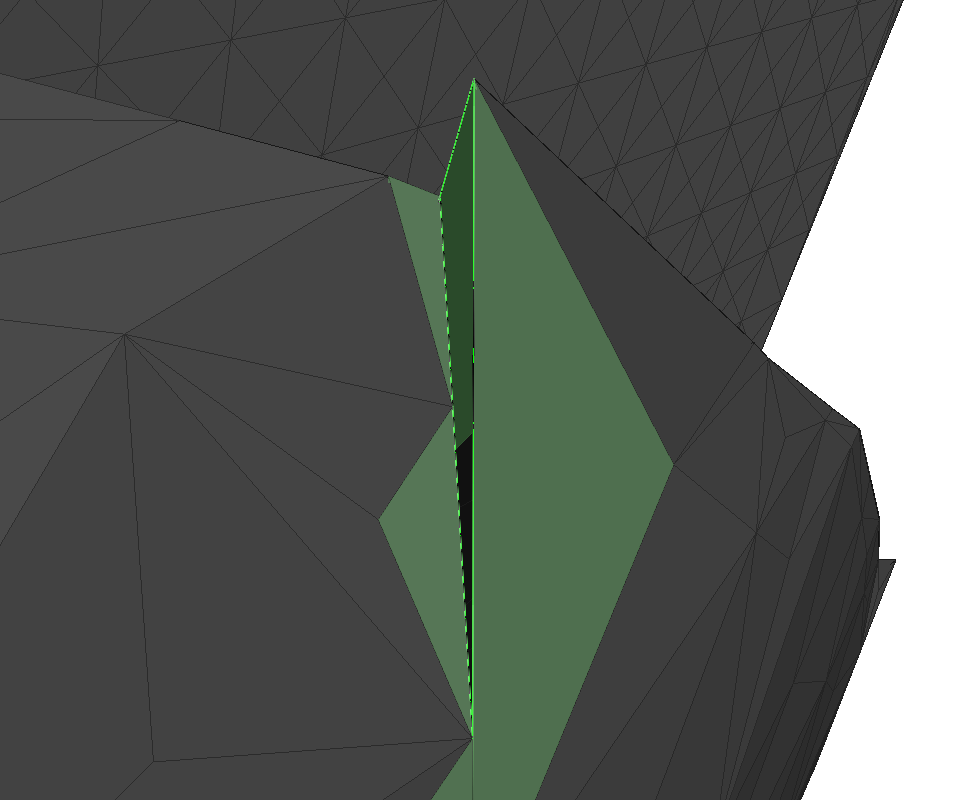
\includegraphics[width=\textwidth]{td_cylinder_head_hole}
		\caption{hole}
		\label{fig:td_cylinder_head_hole}
	\end{subfigure}
	\caption[Tri-dexel T-vertices and holes]{
		Details of the \cylinderhead scene.
		Boundary edges are marked in green.
		The renderings show the creation of T-vertices and holes at the border of normal and sliced cells.
		The hole is created at the border of a cell and a sliced cell, which is discussed in \cref{fig:tri_dexel_hole_creation}.
		The meshes have been extracted using the tri-dexel approach with cell slicing at a grid resolution of 100.
	}
	\label{fig:td_cylinder_head_issues}
\end{figure}

\Cref{tbl:tri_dexel_boundary edges} contains the number of boundary edges for the tested resolutions and the tri-dexel variant using cell slicing.

\begin{table}
	\centering
	\begin{tabular}{l|r|r|r|r}
		scene          & \multicolumn{4}{c}{resolution} \\
		&   50 &  100 &  200 &   400 \\
		\midrule
		\cubes        &    0 &    0 &    0 &     0 \\
		\cylindersd   &    0 &  128 &  238 &   846 \\
		\cylinders    &    0 &    0 &    0 &     0 \\
		\cylinderhead &  871 & 1880 & 4136 &  4966 \\
		\impeller     & 1129 & 2380 & 4654 & 11940 \\
		\impellerhalf &  574 & 1191 & 3033 &  6050 \\
		\turbine      & 2006 & 3703 & 7181 & 13803 \\
	\end{tabular}
	\caption[Tri-dexel boundary edges]{
		Created boundary edges by the tri-dexel surface extraction using cell-slicing and the test scenes described in \cref{tbl:test_scenes}.
		The meshes created without cell-slicing do not contain boundary edges.
	}
	\label{tbl:tri_dexel_boundary edges}
\end{table}


\section{Point cloud based}
\label{sec:point_cloud_results}

The point cloud creation and the subsequent reconstruction using the VML's BPA, \cf \cref{sec:point_cloud_reconstruction}, have been benchmarked individually.
Similar to the tri-dexel benchmarks, the resolutions 50, 100, 200 and 400 have been used for the raycaster creating the point clouds.
\Cref{tbl:point_cloud_results} contains the runtime and output size of the created point clouds.

\begin{table}
	\centering
	\begin{tabular}{l|rr|rr|rr|rr}
		resolution    & \multicolumn{2}{c}{50} & \multicolumn{2}{c}{100} & \multicolumn{2}{c}{200} & \multicolumn{2}{c}{400} \\
		scene         & p\sub{out} & time & p\sub{out} & time & p\sub{out} & time & p\sub{out} & time \\
		\midrule
		\cubes        & \SI{14}{\kilo\nothing} & \SI{  3}{\milli\second} & \SI{56}{\kilo\nothing} & \SI{ 12}{\milli\second} & \SI{226}{\kilo\nothing} & \SI{  47}{\milli\second} & \SI{907}{\kilo\nothing} & \SI{ 187}{\milli\second} \\
		\cylindersd   & \SI{ 7}{\kilo\nothing} & \SI{  5}{\milli\second} & \SI{27}{\kilo\nothing} & \SI{ 17}{\milli\second} & \SI{108}{\kilo\nothing} & \SI{  63}{\milli\second} & \SI{436}{\kilo\nothing} & \SI{ 247}{\milli\second} \\
		\cylinders    & \SI{ 7}{\kilo\nothing} & \SI{  3}{\milli\second} & \SI{26}{\kilo\nothing} & \SI{ 11}{\milli\second} & \SI{107}{\kilo\nothing} & \SI{  41}{\milli\second} & \SI{433}{\kilo\nothing} & \SI{ 161}{\milli\second} \\
		\cylinderhead & \SI{15}{\kilo\nothing} & \SI{  7}{\milli\second} & \SI{60}{\kilo\nothing} & \SI{ 23}{\milli\second} & \SI{242}{\kilo\nothing} & \SI{  86}{\milli\second} & \SI{976}{\kilo\nothing} & \SI{ 335}{\milli\second} \\
		\impeller     & \SI{11}{\kilo\nothing} & \SI{ 99}{\milli\second} & \SI{46}{\kilo\nothing} & \SI{353}{\milli\second} & \SI{184}{\kilo\nothing} & \SI{1118}{\milli\second} & \SI{744}{\kilo\nothing} & \SI{3813}{\milli\second} \\
		\impellerhalf & \SI{ 9}{\kilo\nothing} & \SI{ 54}{\milli\second} & \SI{38}{\kilo\nothing} & \SI{193}{\milli\second} & \SI{155}{\kilo\nothing} & \SI{ 600}{\milli\second} & \SI{625}{\kilo\nothing} & \SI{2037}{\milli\second} \\
		\turbine      & \SI{ 7}{\kilo\nothing} & \SI{165}{\milli\second} & \SI{31}{\kilo\nothing} & \SI{650}{\milli\second} & \SI{132}{\kilo\nothing} & \SI{2509}{\milli\second} & \SI{532}{\kilo\nothing} & \SI{9610}{\milli\second} \\
	\end{tabular}
	\caption[Point cloud results]{
		Test results for the point cloud creation.
	}
	\label{tbl:point_cloud_results}
\end{table}

The mesh sizes and timings for the VML's BPA implementation are given in \cref{tbl:bpa_results}.
The ball's radius in the tests is derived from the raycasting resolution and set to 1.5 times the diameter of a cell of the sampling grid created by three axis aligned raycasts.

%TODO consider different table separation: remove pin columns and move into own table with pin and tout
\begin{table}
	\centering
	\begin{tabular}{l|rrr|rrr}
		resolution    & \multicolumn{3}{c}{50} & \multicolumn{3}{c}{100} \\
		scene         & p\sub{in} & t\sub{out} & time & p\sub{in} & t\sub{out} & time \\
		\midrule
		\cubes        & \SI{14}{\kilo\nothing}& \SI{27}{\kilo\nothing} & \SI{53}{\milli\second} & \SI{56}{\kilo\nothing} & \SI{111}{\kilo\nothing} & \SI{222}{\milli\second} \\
		\cylindersd   & \SI{ 7}{\kilo\nothing}& \SI{13}{\kilo\nothing} & \SI{22}{\milli\second} & \SI{27}{\kilo\nothing} & \SI{ 53}{\kilo\nothing} & \SI{ 95}{\milli\second} \\
		\cylinders    & \SI{ 7}{\kilo\nothing}& \SI{13}{\kilo\nothing} & \SI{22}{\milli\second} & \SI{26}{\kilo\nothing} & \SI{ 53}{\kilo\nothing} & \SI{ 94}{\milli\second} \\
		\cylinderhead & \SI{15}{\kilo\nothing}& \SI{27}{\kilo\nothing} & \SI{60}{\milli\second} & \SI{60}{\kilo\nothing} & \SI{110}{\kilo\nothing} & \SI{223}{\milli\second} \\
		\impeller     & \SI{11}{\kilo\nothing}& \SI{20}{\kilo\nothing} & \SI{48}{\milli\second} & \SI{46}{\kilo\nothing} & \SI{ 91}{\kilo\nothing} & \SI{200}{\milli\second} \\
		\impellerhalf & \SI{ 9}{\kilo\nothing}& \SI{17}{\kilo\nothing} & \SI{36}{\milli\second} & \SI{38}{\kilo\nothing} & \SI{ 76}{\kilo\nothing} & \SI{161}{\milli\second} \\
		\turbine      & \SI{ 7}{\kilo\nothing}& \SI{ 9}{\kilo\nothing} & \SI{20}{\milli\second} & \SI{31}{\kilo\nothing} & \SI{ 53}{\kilo\nothing} & \SI{142}{\milli\second} \\
		
		\multicolumn{1}{l}{\bigskip} \\
		
		resolution    & \multicolumn{3}{c}{200} & \multicolumn{3}{c}{400} \\
		scene         & p\sub{in} & t\sub{out} & time & p\sub{in} & t\sub{out} & time \\
		\midrule
		\cubes        & \SI{226}{\kilo\nothing}& \SI{449}{\kilo\nothing} & \SI{1022}{\milli\second} & \SI{907}{\kilo\nothing}& \SI{1807}{\kilo\nothing} & \SI{5106}{\milli\second} \\
		\cylindersd   & \SI{108}{\kilo\nothing}& \SI{217}{\kilo\nothing} & \SI{ 442}{\milli\second} & \SI{436}{\kilo\nothing}& \SI{ 871}{\kilo\nothing} & \SI{1999}{\milli\second} \\
		\cylinders    & \SI{107}{\kilo\nothing}& \SI{215}{\kilo\nothing} & \SI{ 421}{\milli\second} & \SI{433}{\kilo\nothing}& \SI{ 865}{\kilo\nothing} & \SI{1902}{\milli\second} \\
		\cylinderhead & \SI{242}{\kilo\nothing}& \SI{454}{\kilo\nothing} & \SI{ 946}{\milli\second} & \SI{976}{\kilo\nothing}& \SI{1850}{\kilo\nothing} & \SI{4263}{\milli\second} \\
		\impeller     & \SI{184}{\kilo\nothing}& \SI{368}{\kilo\nothing} & \SI{ 859}{\milli\second} & \SI{744}{\kilo\nothing}& \SI{1485}{\kilo\nothing} & \SI{3710}{\milli\second} \\
		\impellerhalf & \SI{155}{\kilo\nothing}& \SI{309}{\kilo\nothing} & \SI{ 695}{\milli\second} & \SI{625}{\kilo\nothing}& \SI{1248}{\kilo\nothing} & \SI{3135}{\milli\second} \\
		\turbine      & \SI{132}{\kilo\nothing}& \SI{246}{\kilo\nothing} & \SI{ 613}{\milli\second} & \SI{532}{\kilo\nothing}& \SI{1049}{\kilo\nothing} & \SI{2222}{\milli\second} \\
	\end{tabular}
	\caption[BPA results]{
		Test results for surface reconstruction using the VML's internal BPA implementation excluding the time required to generate the point cloud, \cf \cref{tbl:point_cloud_results}.
	}
	\label{tbl:bpa_results}
\end{table}

The CPU utilization during a single run of the BPA surface extraction of the \impeller scene with a grid resolution of 400 is shown in \cref{fig:bpa_hq_impeller_cpu}.

\begin{figure}
	\centering
	\begin{tikzpicture}
	\begin{axis}[
		width=0.95\textwidth,
		height=0.5\textwidth,
		xlabel={Wall clock time in \si{\second}},
		ylabel={CPU utilization in \si{\percent}},
		ymin=0,
		ymax=100,
		ytick={0,20,...,100},
		%xtick={0,2,...,100}
	]
	\addplot table [x=time, y=utilization, col sep=comma]{spreadsheets/bpa_hq_impeller_cpu.csv};
	\end{axis}
	\end{tikzpicture}
	\caption[BPA CPU utilization]{
		CPU utilization during point cloud creation and a run of the BPA with a grid resolution of 400 on the \impeller scene.
	}
	\label{fig:bpa_hq_impeller_cpu}
\end{figure}

\Cref{fig:bpa_results} shows renderings of the result meshes on point clouds created with a resolution of 400.

\begin{figure}
	\centering
	\begin{subfigure}[b]{0.34\textwidth}
		\centering
		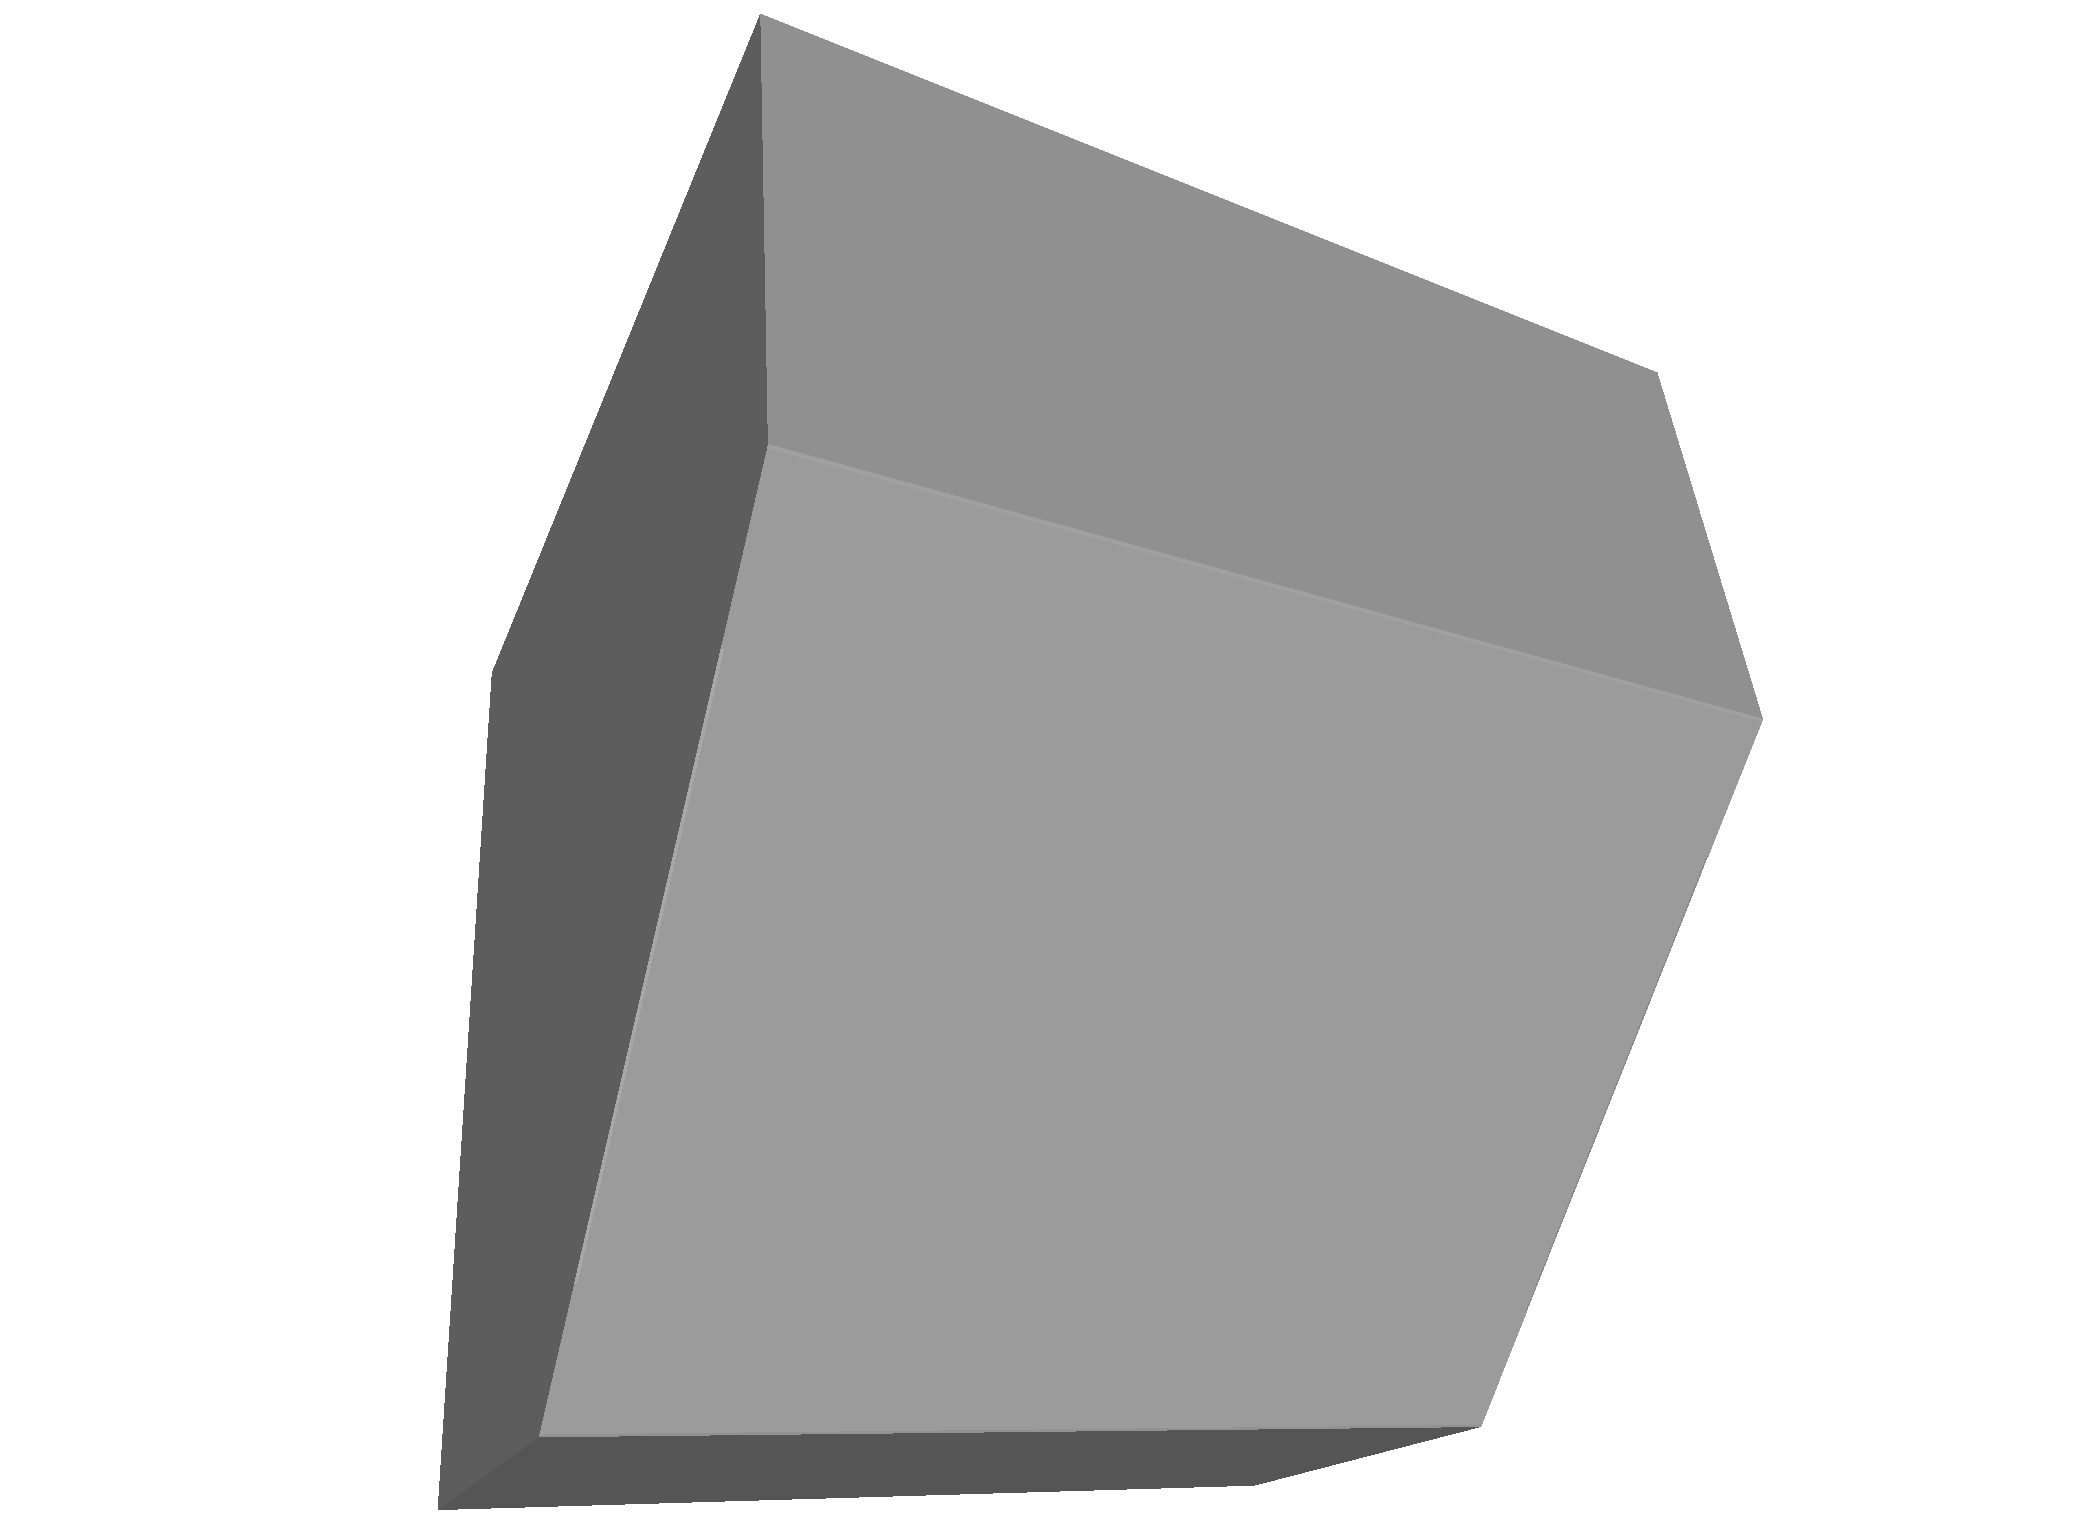
\includegraphics[width=\textwidth]{bpa_cube2}
		\caption{\cubes}
		\label{fig:bpa_cube2}
	\end{subfigure}
	\hspace{1cm}
	\begin{subfigure}[b]{0.34\textwidth}
		\centering
		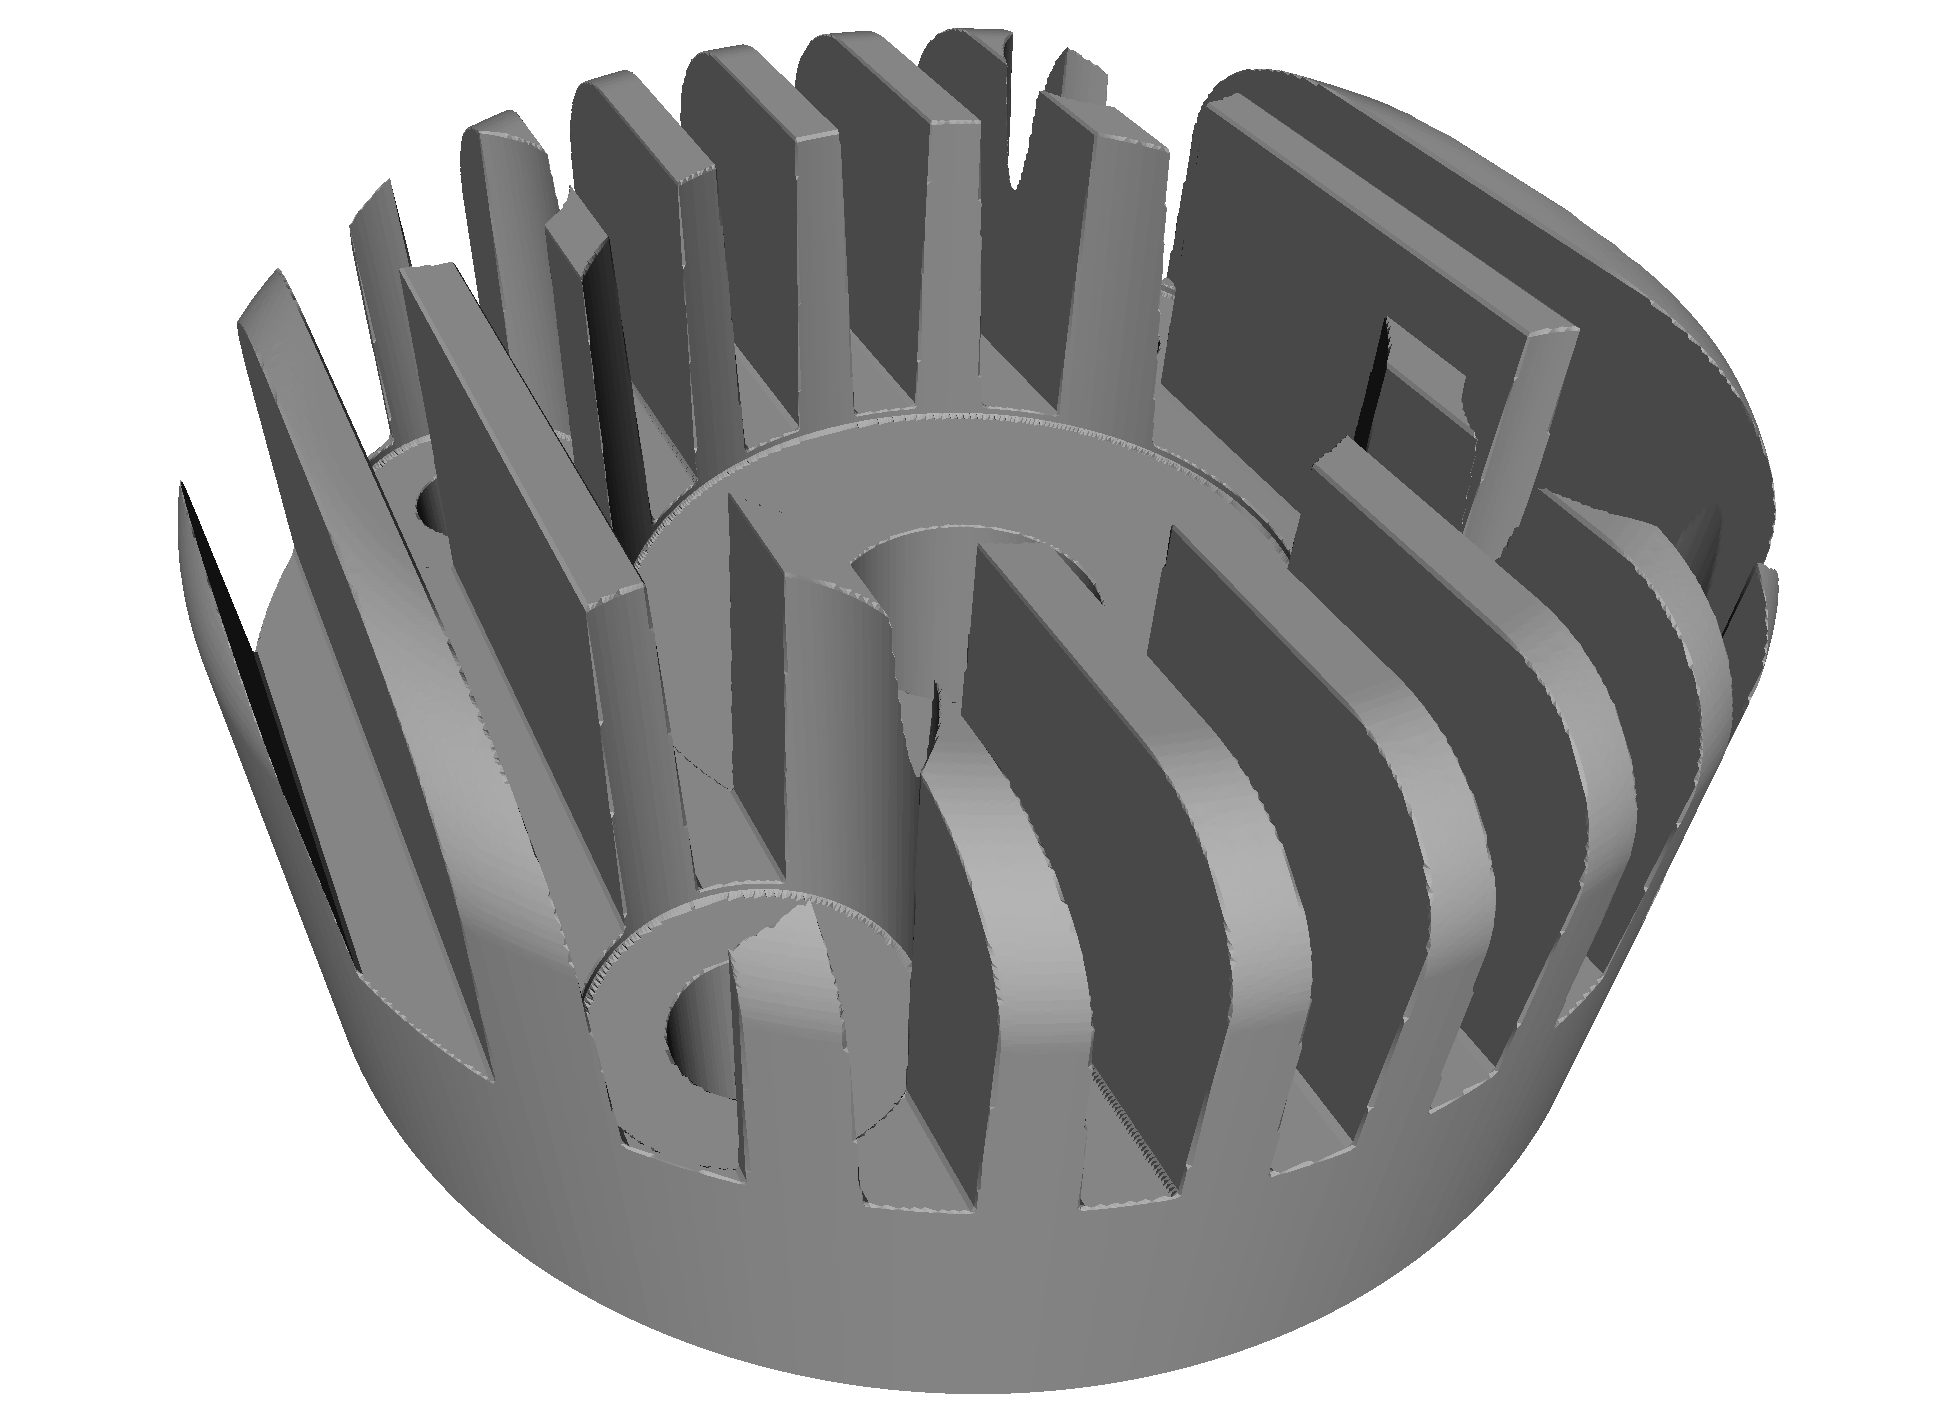
\includegraphics[width=\textwidth]{bpa_cylinder_head}
		\caption{\cylinderhead}
		\label{fig:bpa_cylinder_head}
	\end{subfigure}
	\begin{subfigure}[b]{0.34\textwidth}
		\centering
		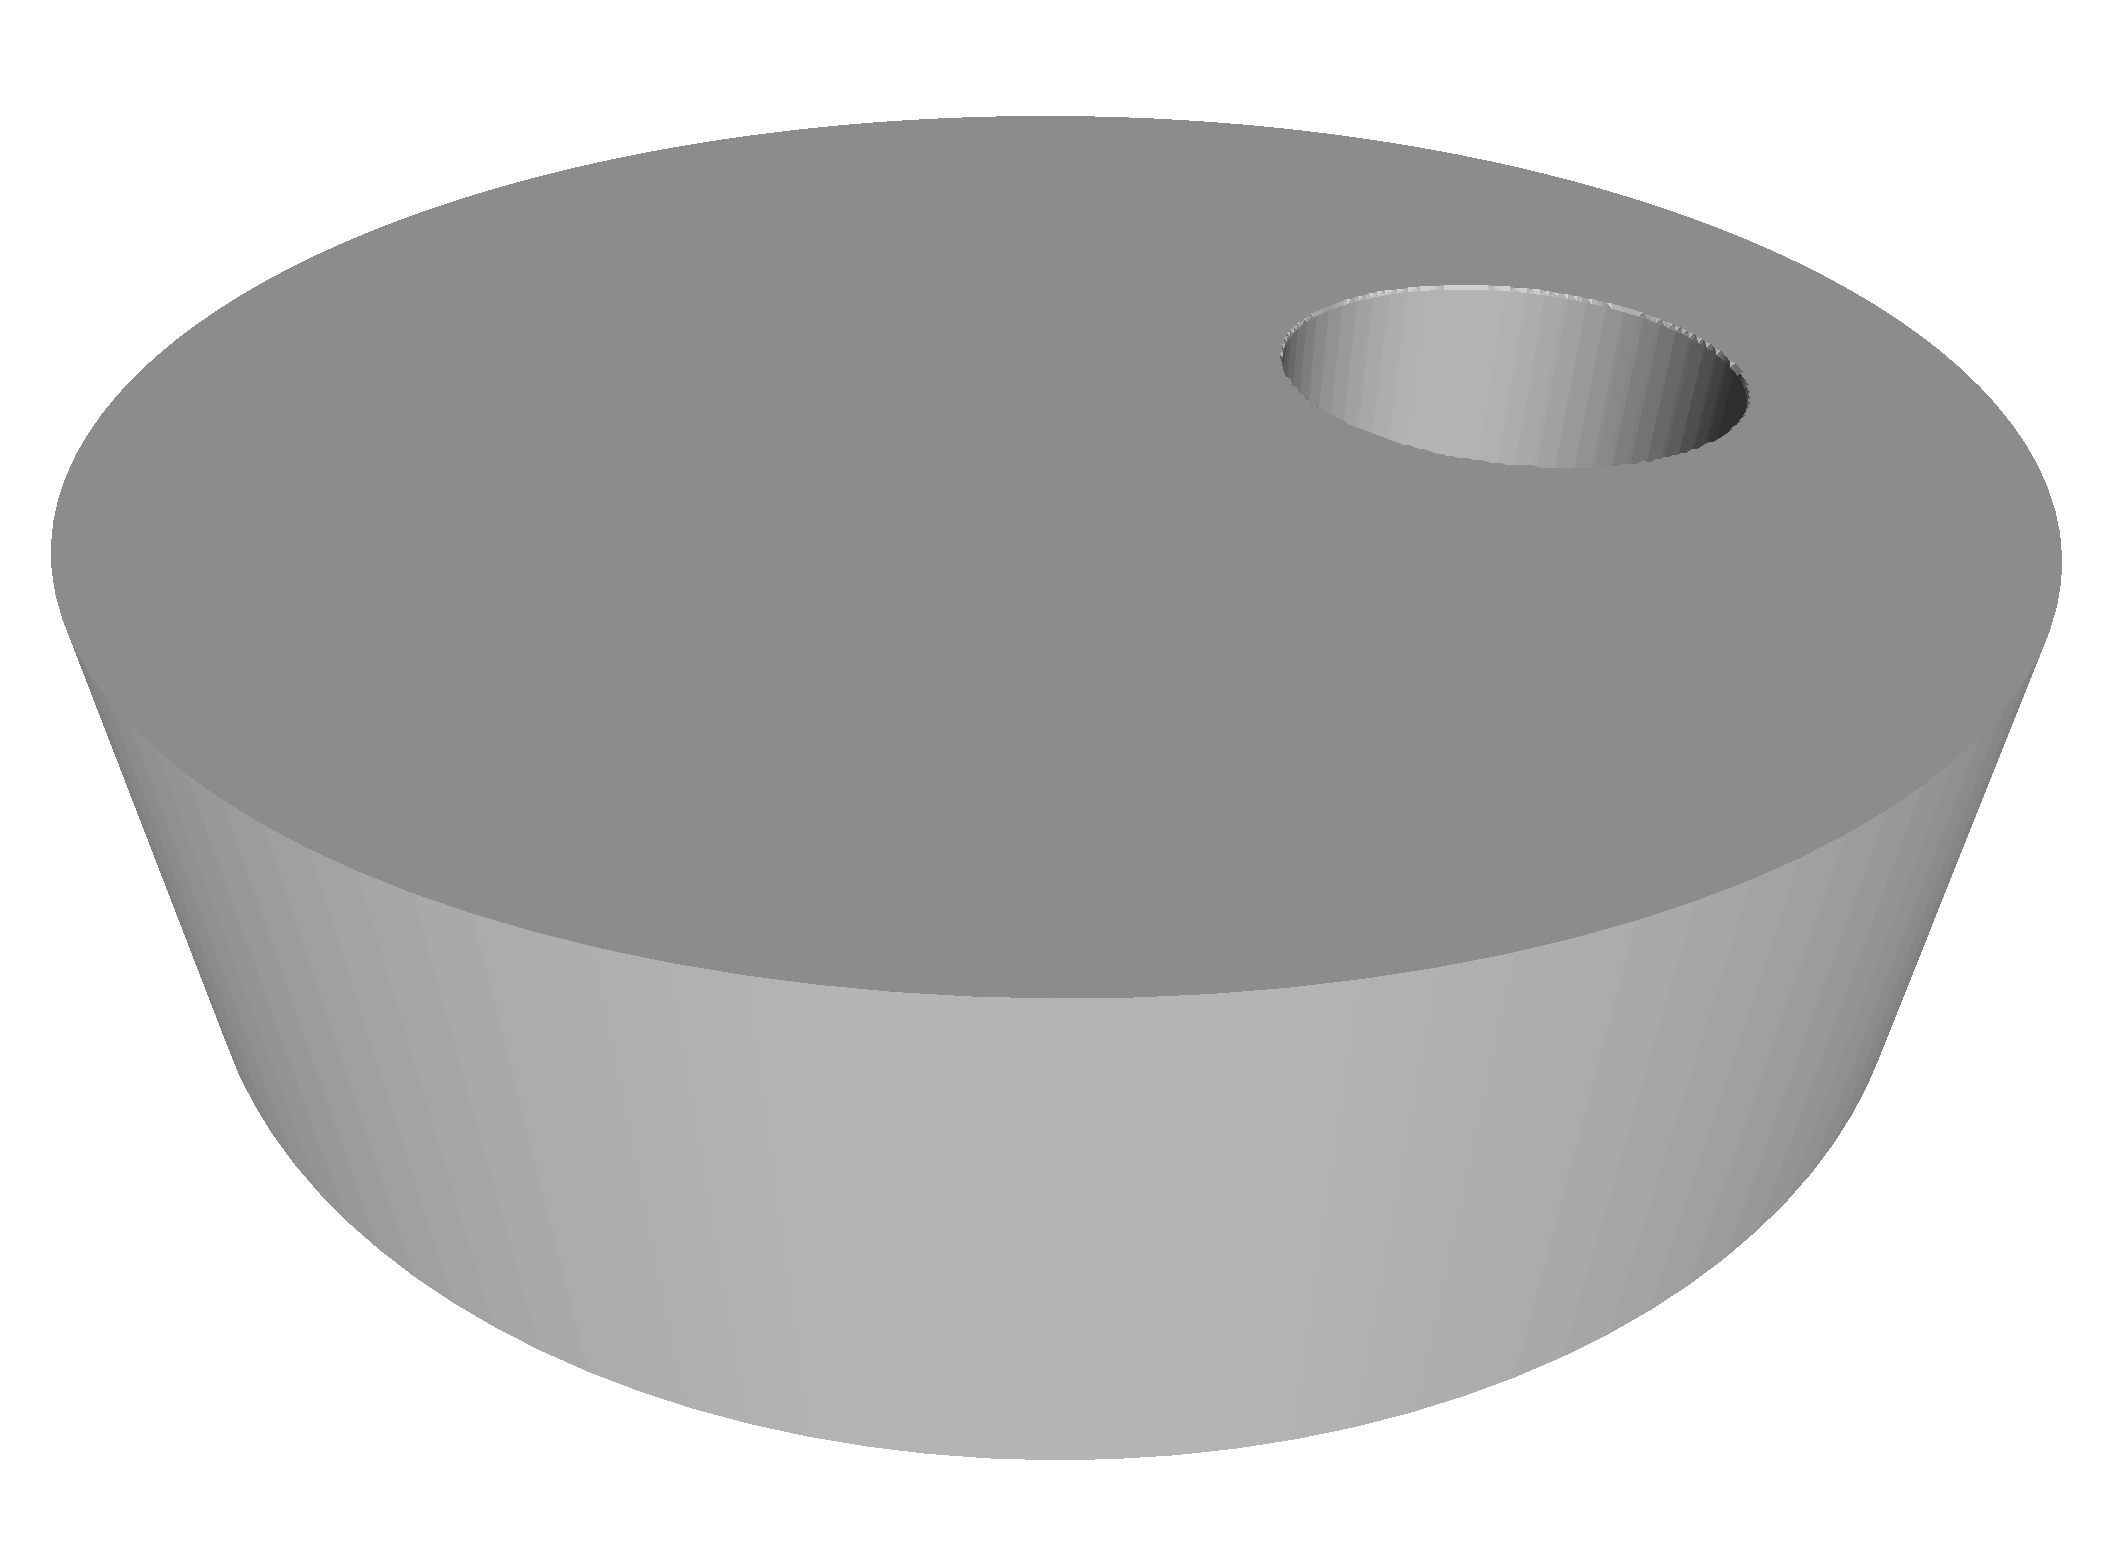
\includegraphics[width=\textwidth]{bpa_cylinders}
		\caption{\cylinders}
		\label{fig:bpa_cylinders}
	\end{subfigure}
	\hspace{1cm}
	\begin{subfigure}[b]{0.34\textwidth}
		\centering
		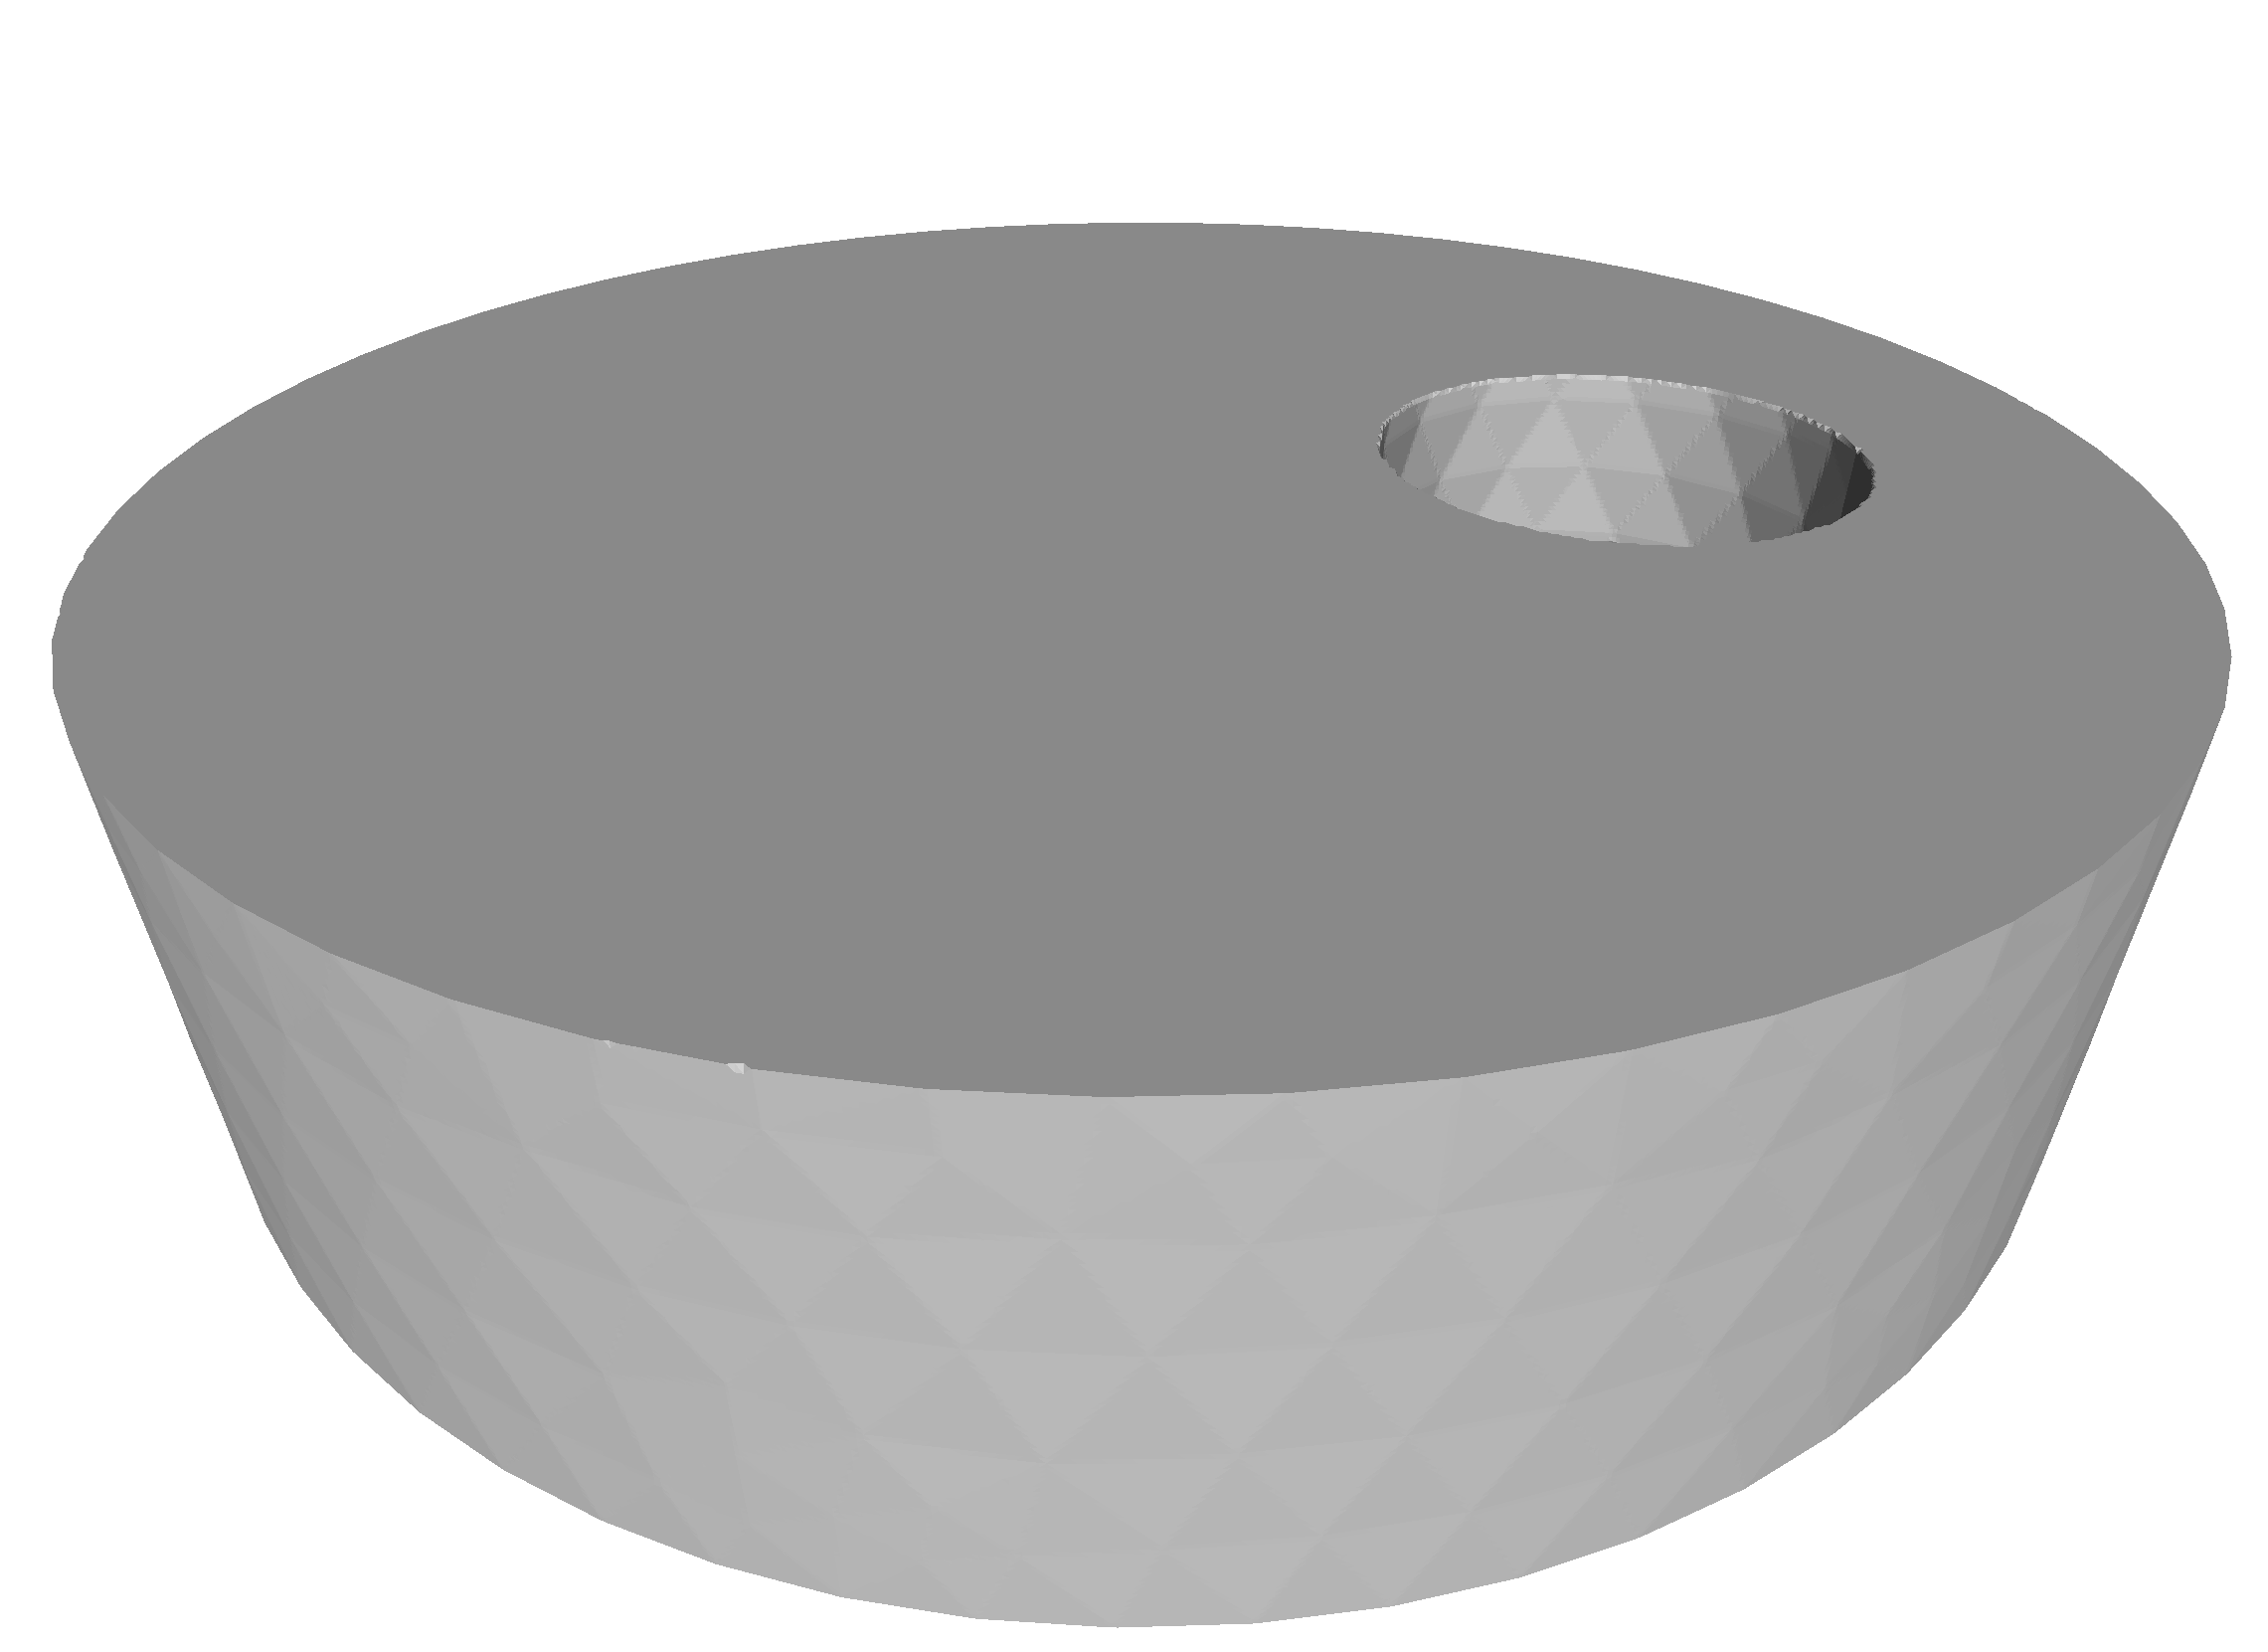
\includegraphics[width=\textwidth]{bpa_cylinders_d}
		\caption{\cylindersd}
		\label{fig:bpa_cylinders_d}
	\end{subfigure}
	\begin{subfigure}[b]{0.34\textwidth}
		\centering
		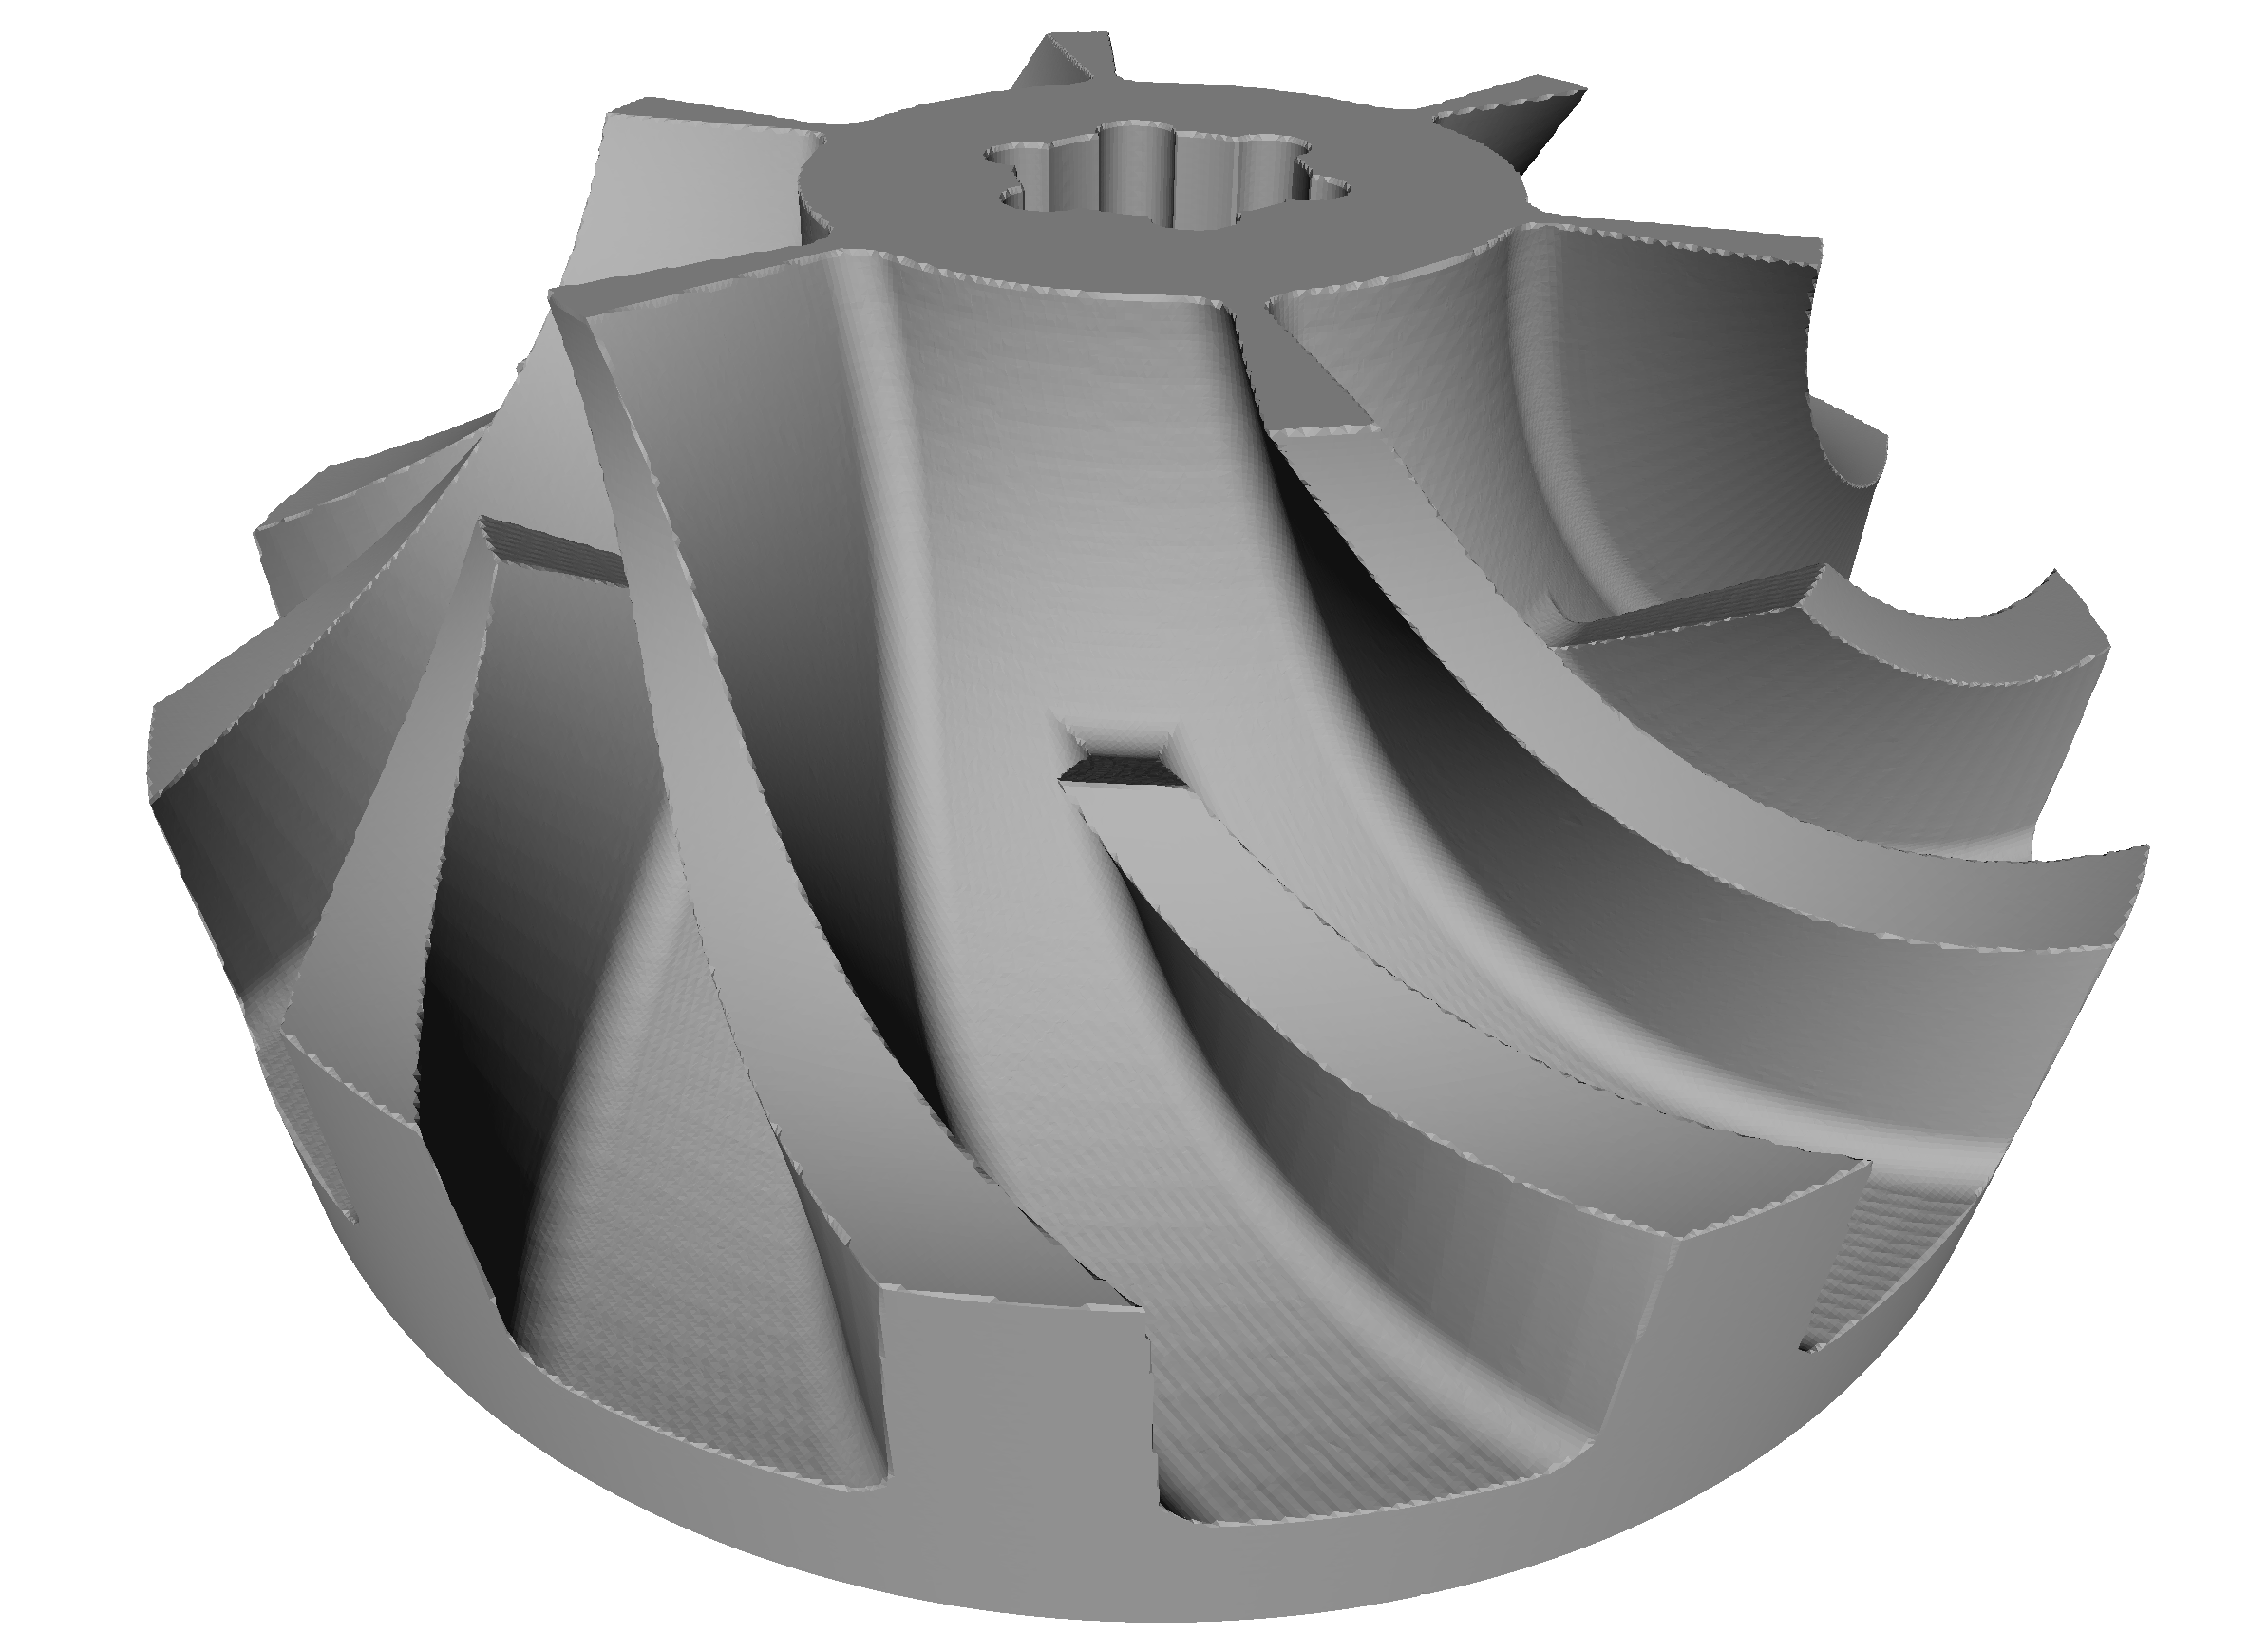
\includegraphics[width=\textwidth]{bpa_hq_impeller}
		\caption{\impeller}
		\label{fig:bpa_hq_impeller}
	\end{subfigure}
	\hspace{1cm}
	\begin{subfigure}[b]{0.34\textwidth}
		\centering
		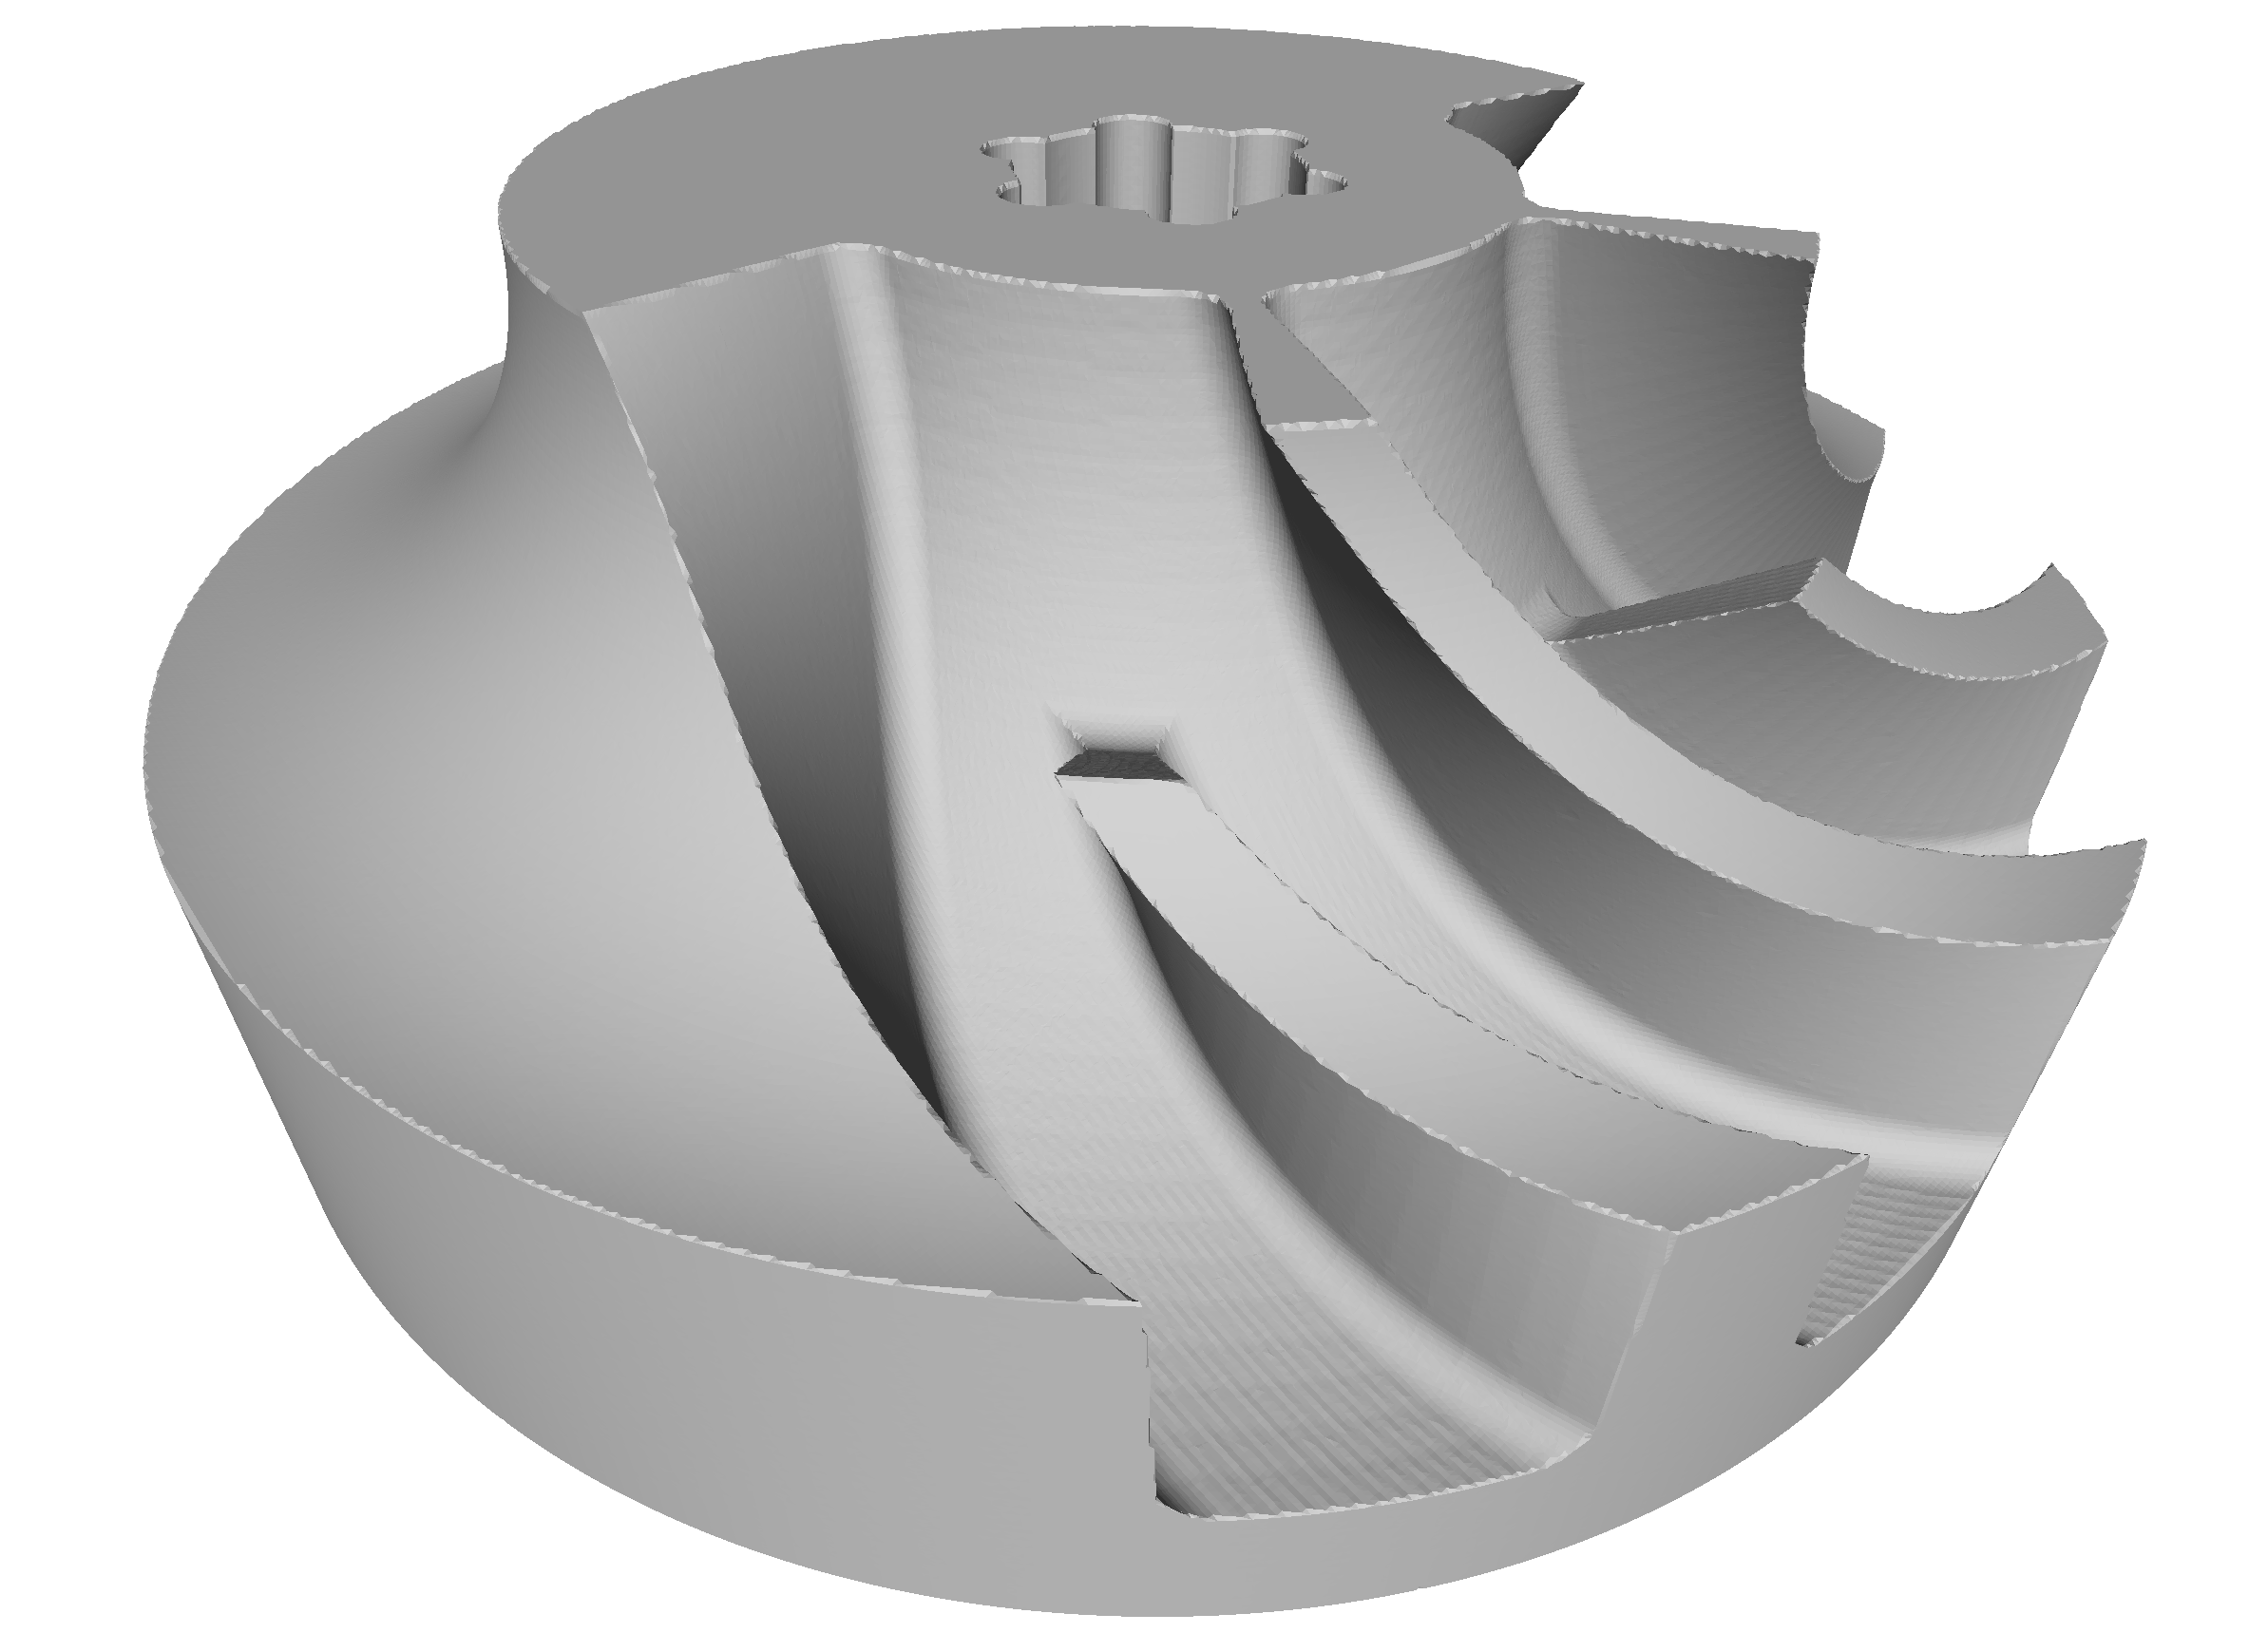
\includegraphics[width=\textwidth]{bpa_hq_impeller_2}
		\caption{\impellerhalf}
		\label{fig:bpa_hq_impeller_2}
	\end{subfigure}
	\begin{subfigure}[b]{0.33\textwidth}
		\centering
		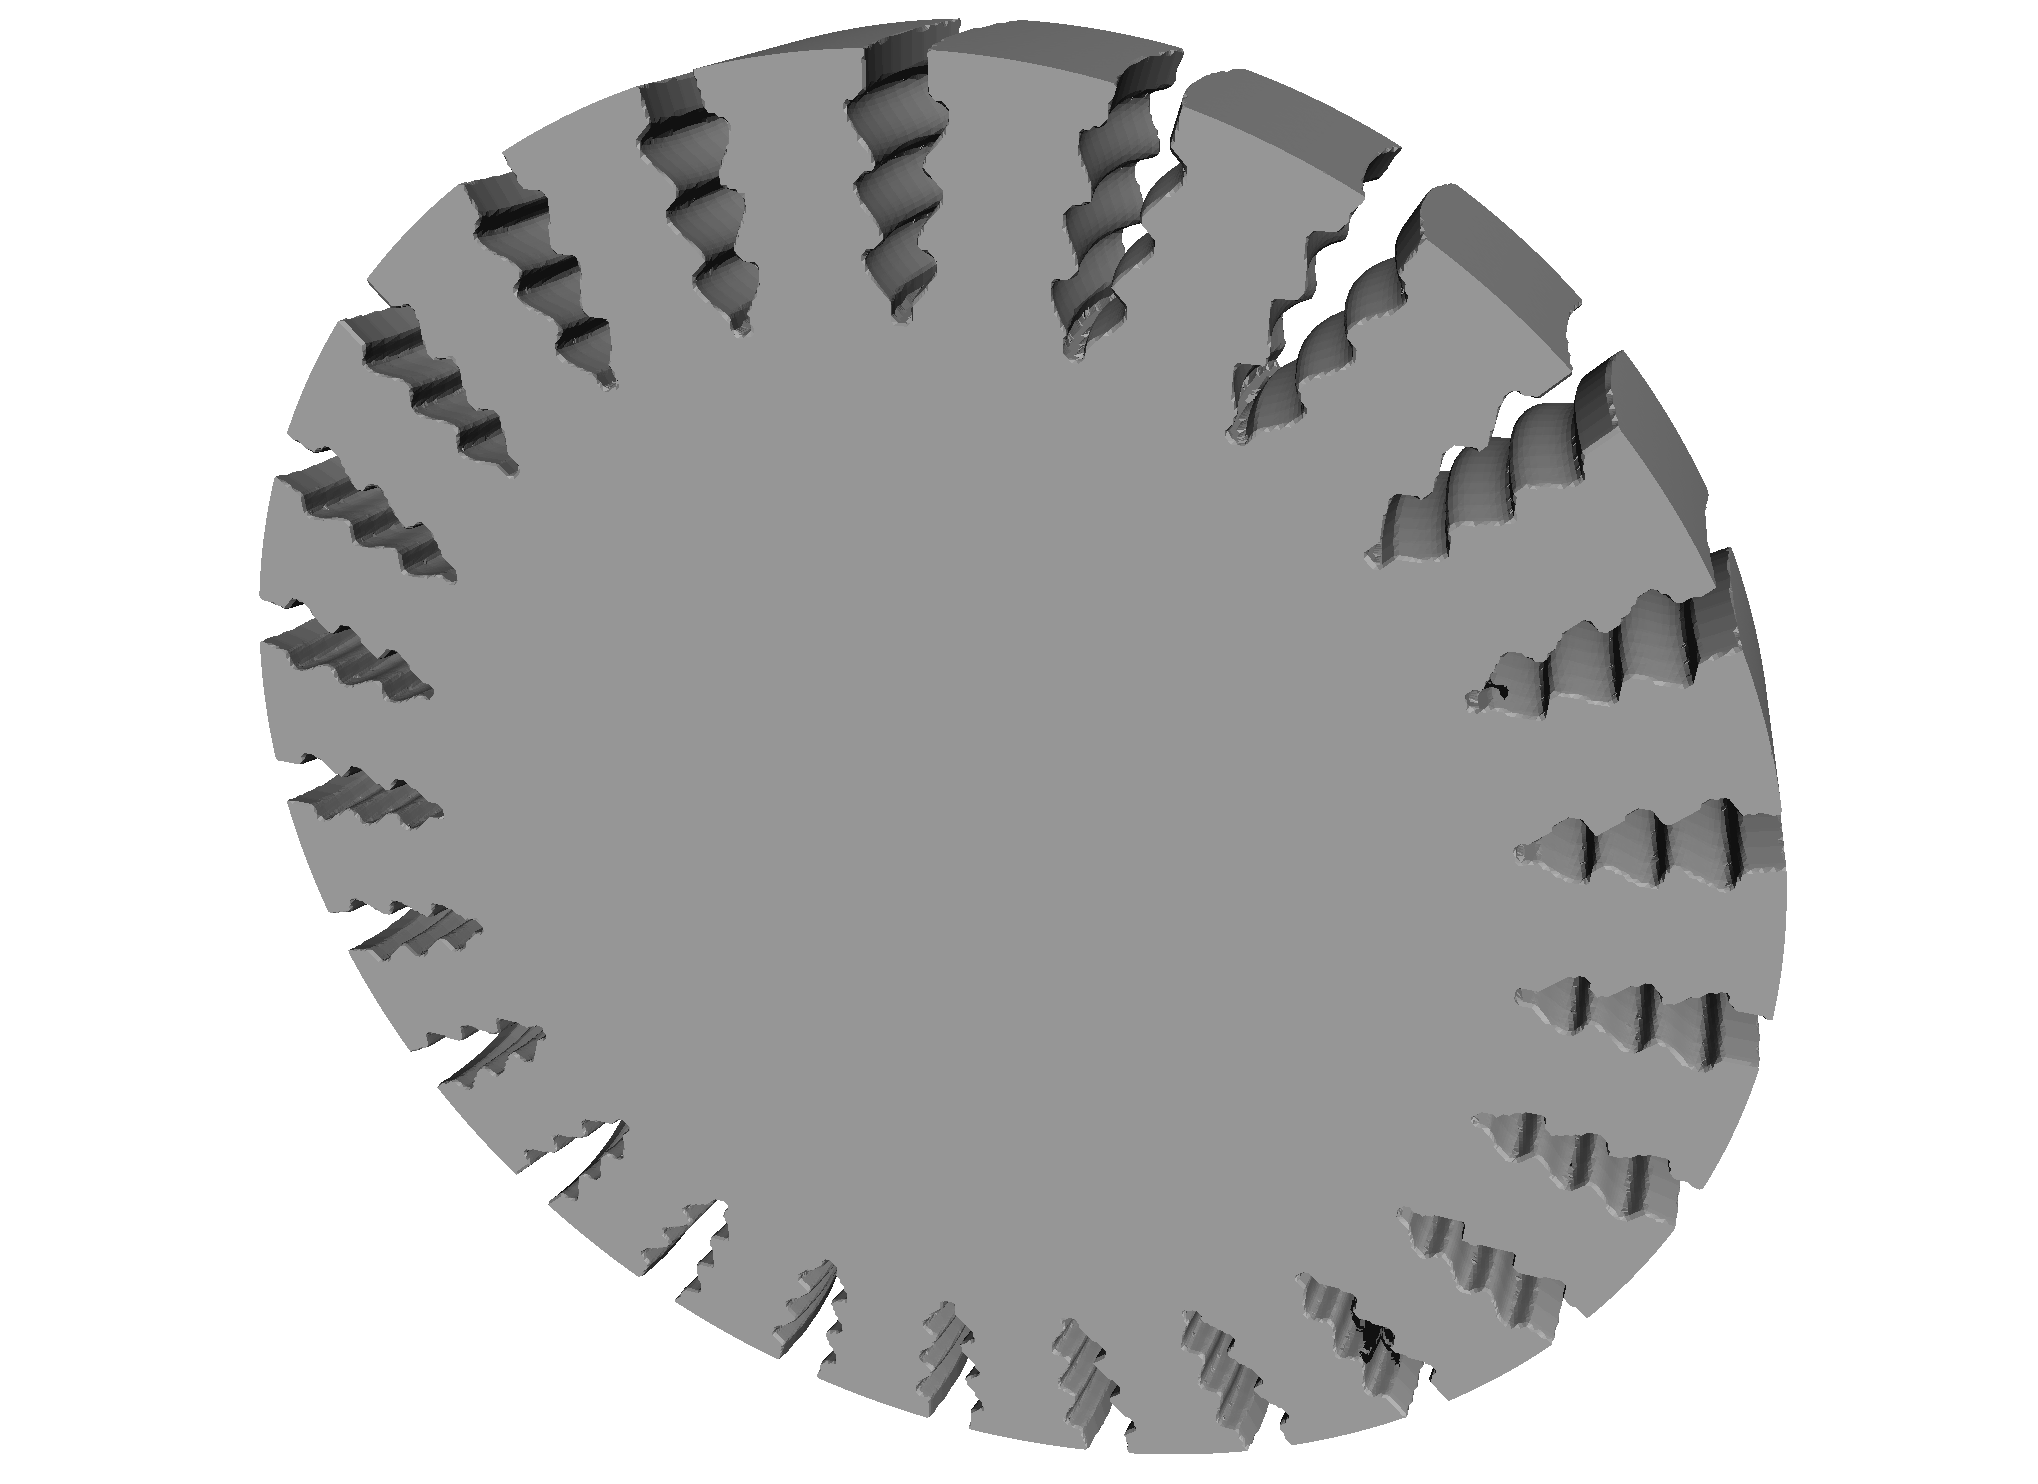
\includegraphics[width=\textwidth]{bpa_turbine}
		\caption{\turbine}
		\label{fig:bpa_turbine}
	\end{subfigure}
	\caption[BPA result renderings]{
		Renderings of the result meshes after applying the BPA reconstruction approach on a point cloud created with a resolution of 400 on the selected test scenes in \cref{tbl:test_scenes}.
	}
	\label{fig:bpa_results}
\end{figure}

Several concave and convex edges of the \cylinderhead scene which were not correctly reconstructed are shown in \cref{fig:bpa_cylinder_head_edges}.

\begin{figure}
	\centering
	\begin{subfigure}[b]{0.49\textwidth}
		\centering
		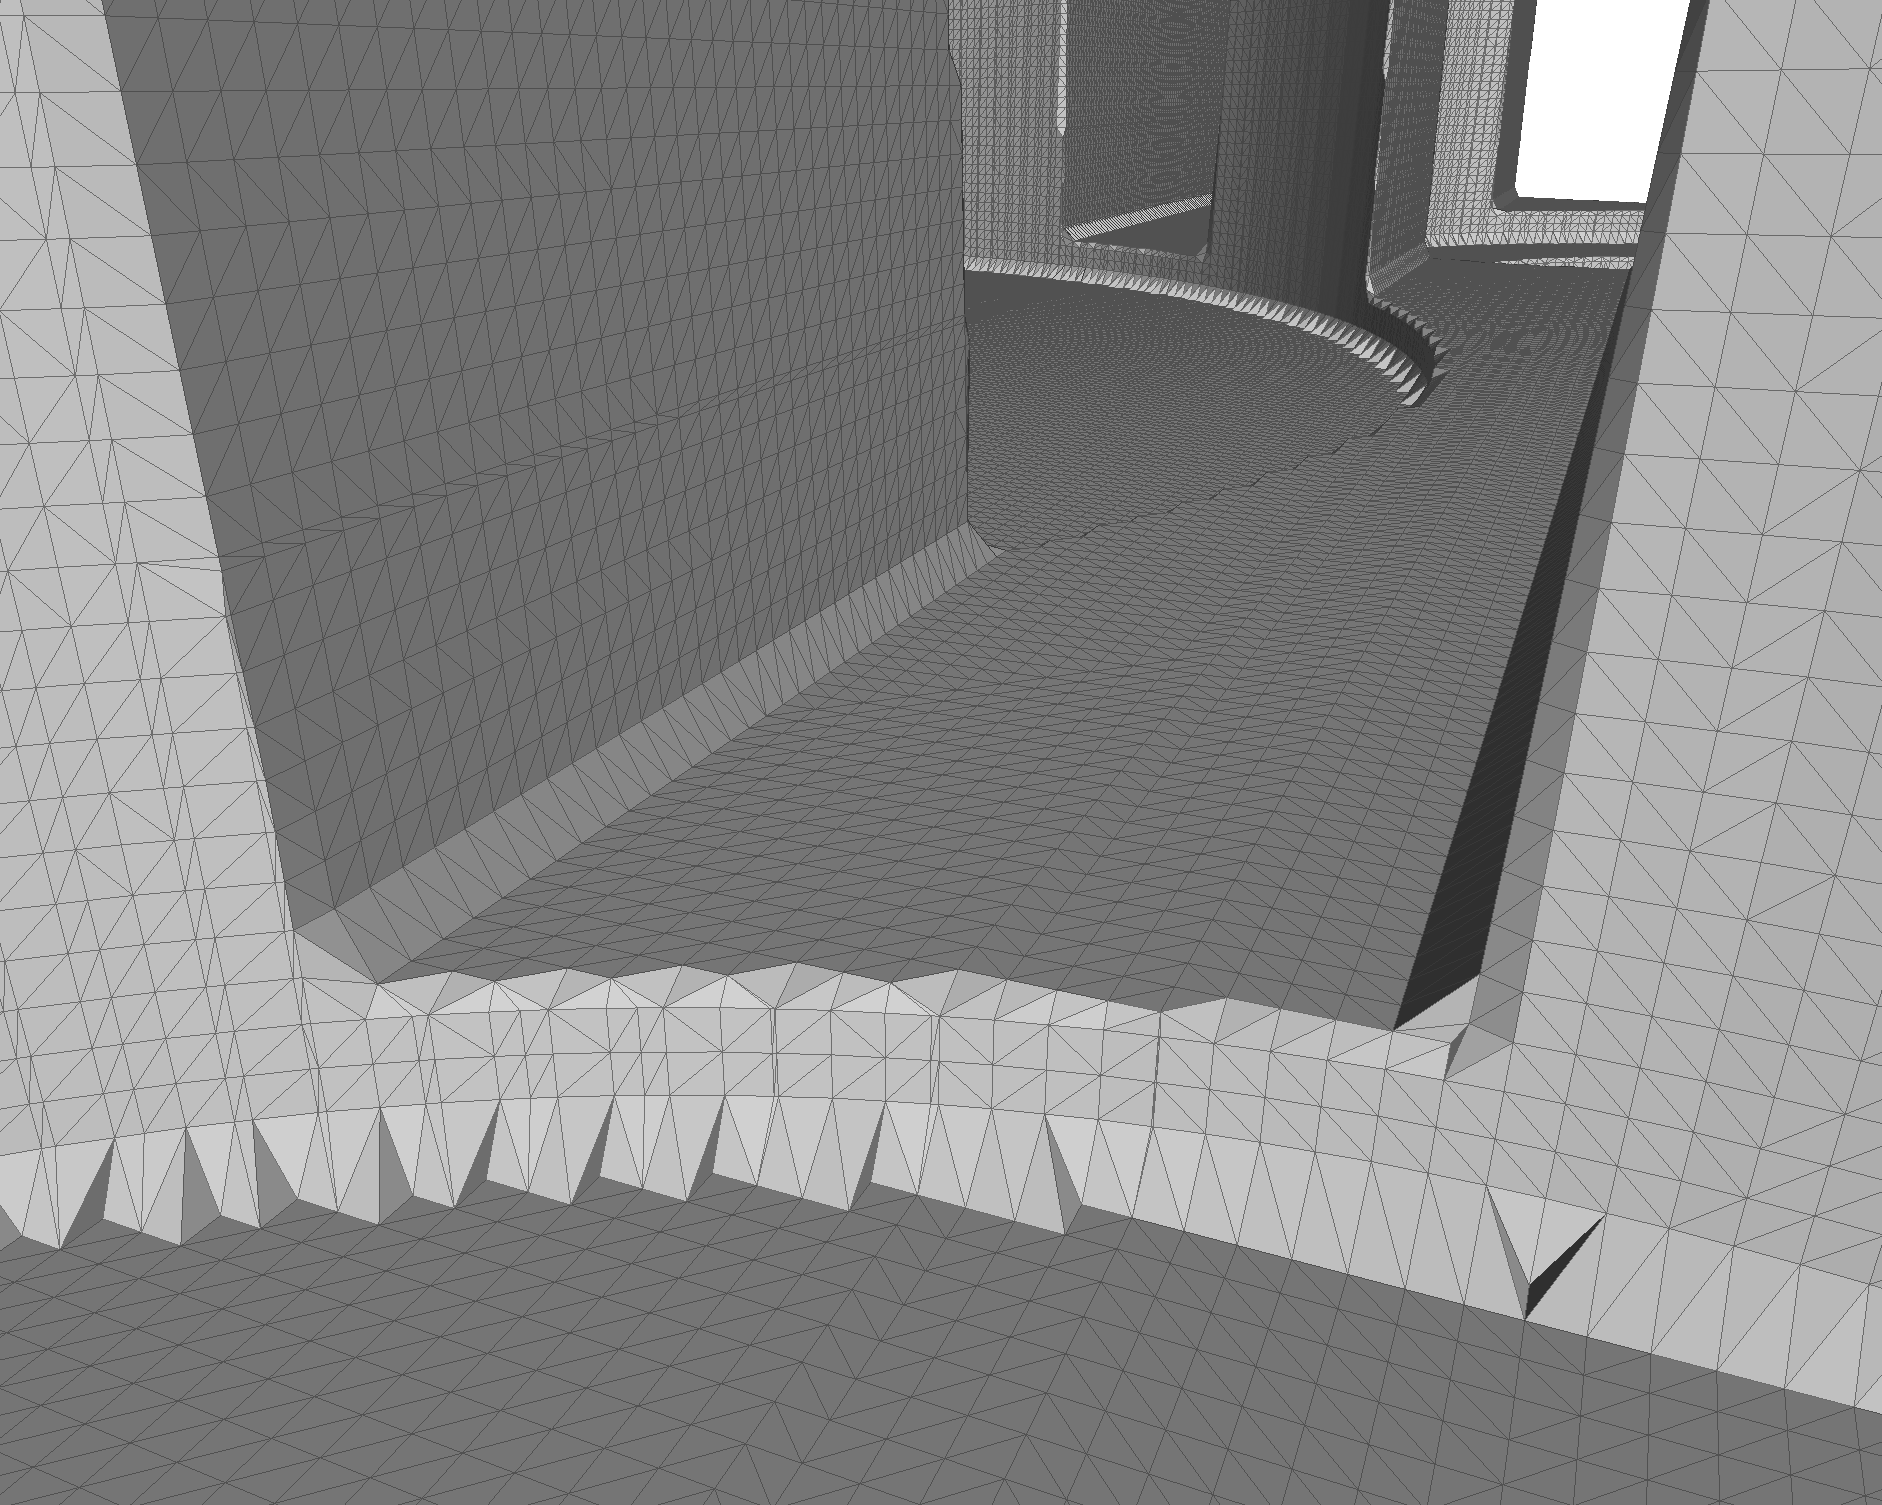
\includegraphics[width=\textwidth]{bpa_cylinder_head_edges}
		\caption{\cylinderhead edges}
		\label{fig:bpa_cylinder_head_edges}
	\end{subfigure}
	\begin{subfigure}[b]{0.49\textwidth}
		\centering
		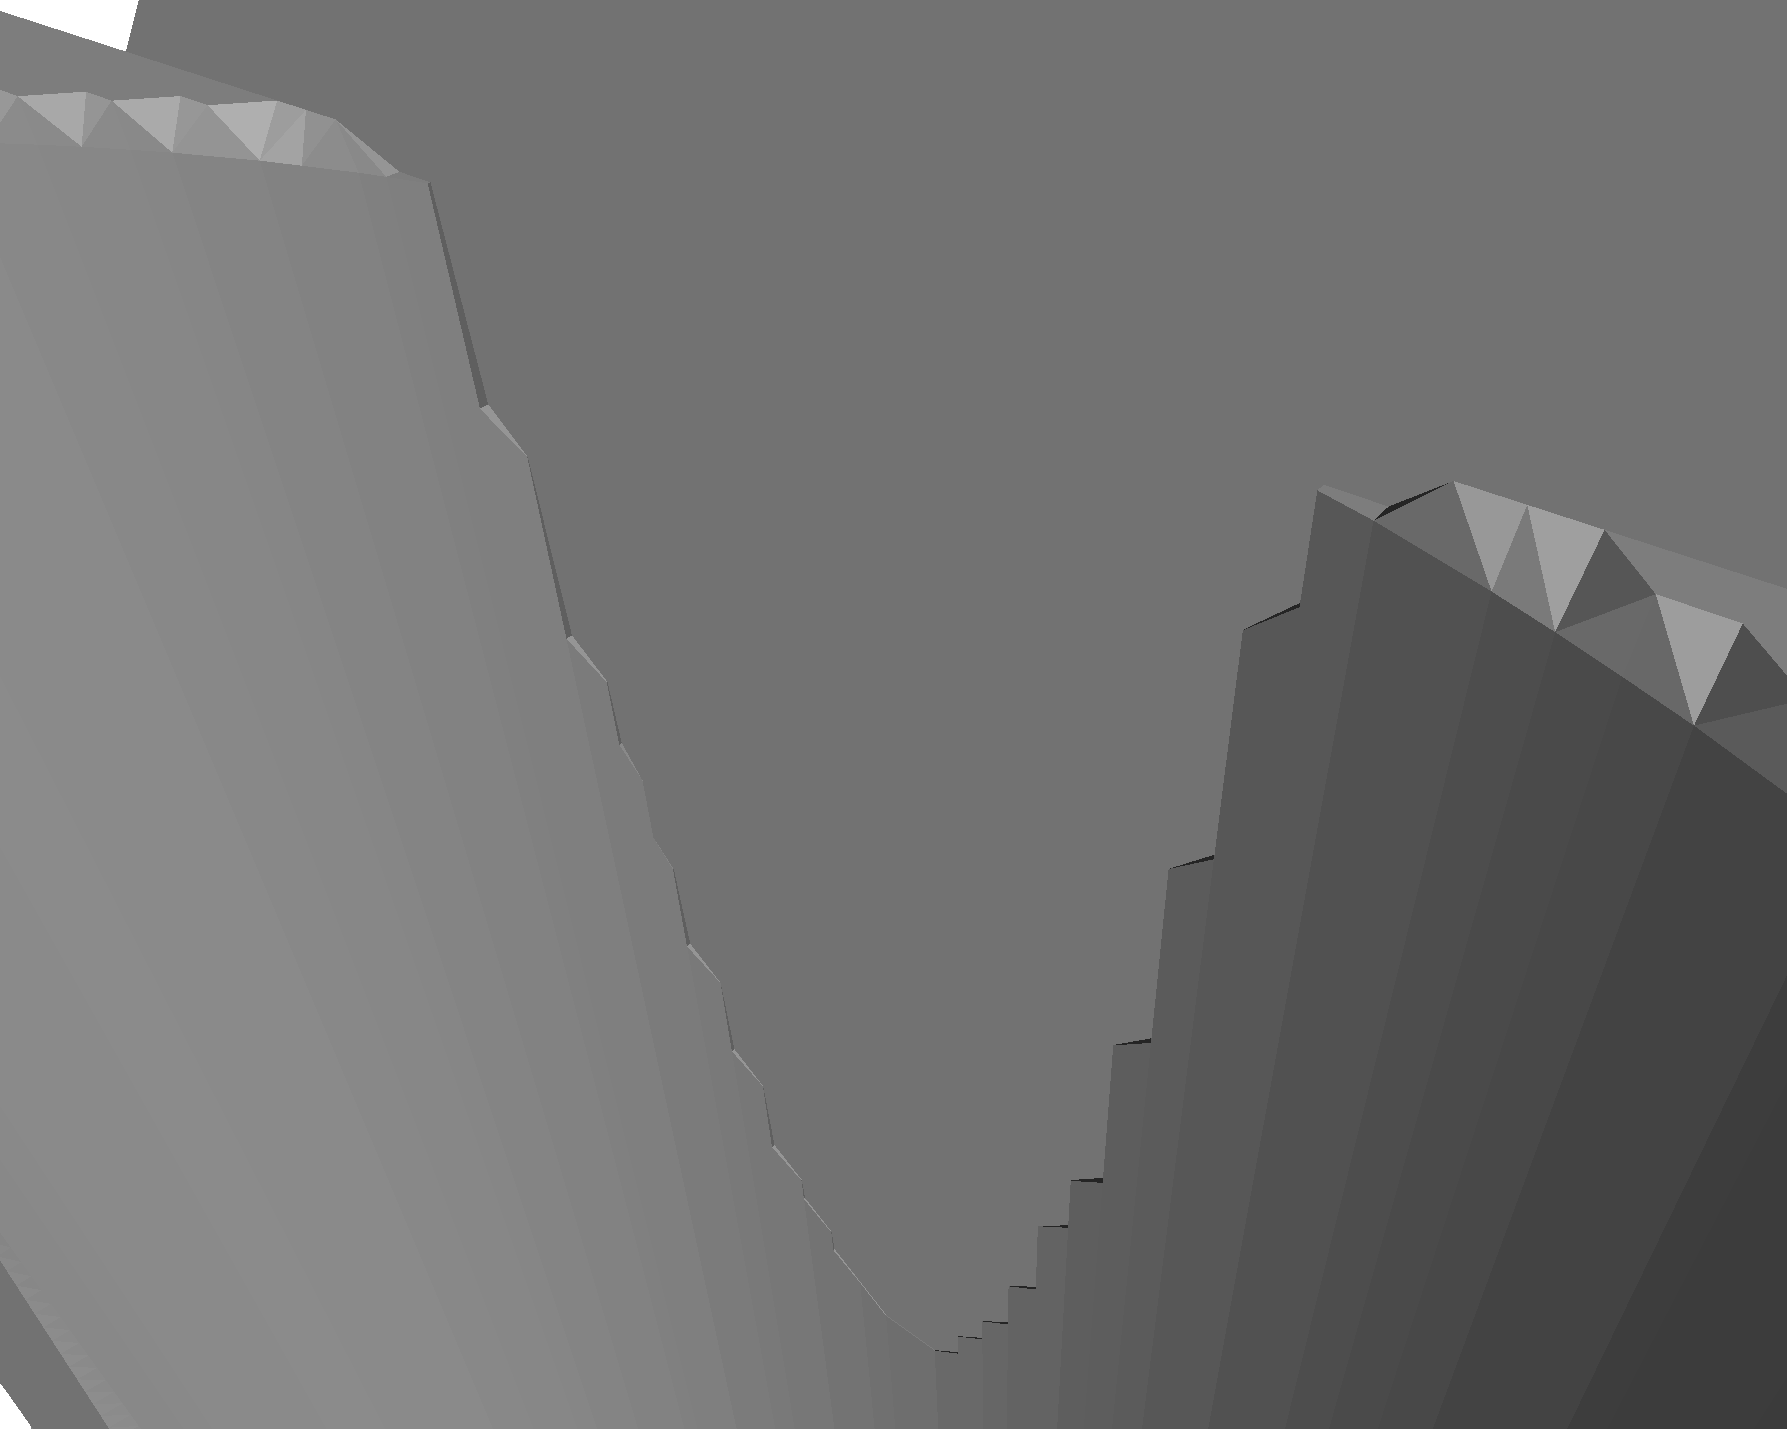
\includegraphics[width=\textwidth]{bpa_cylinder_head_thin_fin}
		\caption{\cylinderhead drilling at fin}
		\label{fig:bpa_cylinder_head_thin_fin}
	\end{subfigure}
	\caption[BPA result details]{
		Details of the \cylinderhead scene.
		The meshes have been extracted using the BPA approach with a resolution of 400.
	}
	\label{fig:bpa_cylinder_head_details}
\end{figure}

\Cref{fig:bpa_grooves} shows the grooves of the \turbine reconstructed from point clouds with various resolutions.

\begin{figure}
	\centering
	\begin{subfigure}[b]{0.24\textwidth}
		\centering
		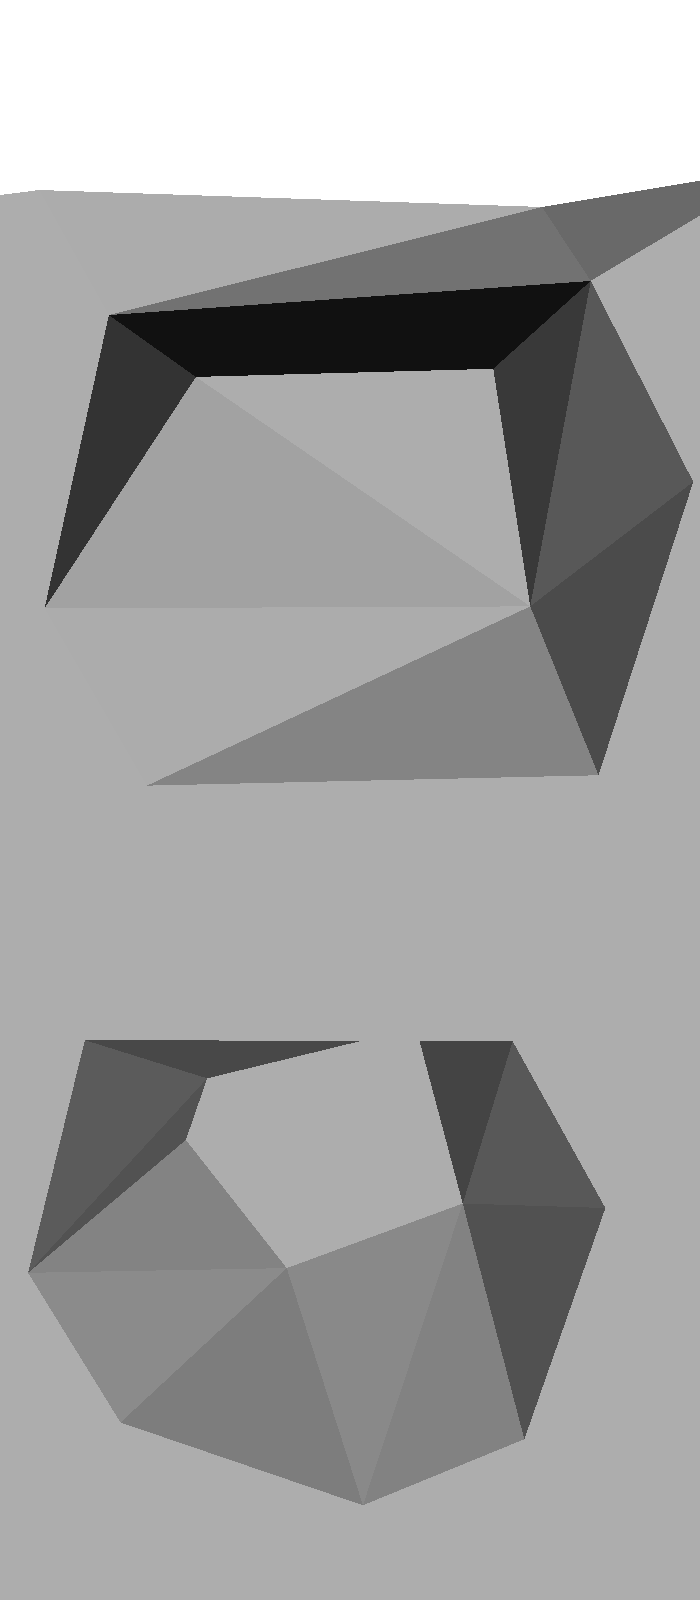
\includegraphics[width=\textwidth]{bpa_turbine_groove_50}
		\caption{50}
		\label{fig:bpa_turbine_groove_50}
	\end{subfigure}
	\begin{subfigure}[b]{0.24\textwidth}
		\centering
		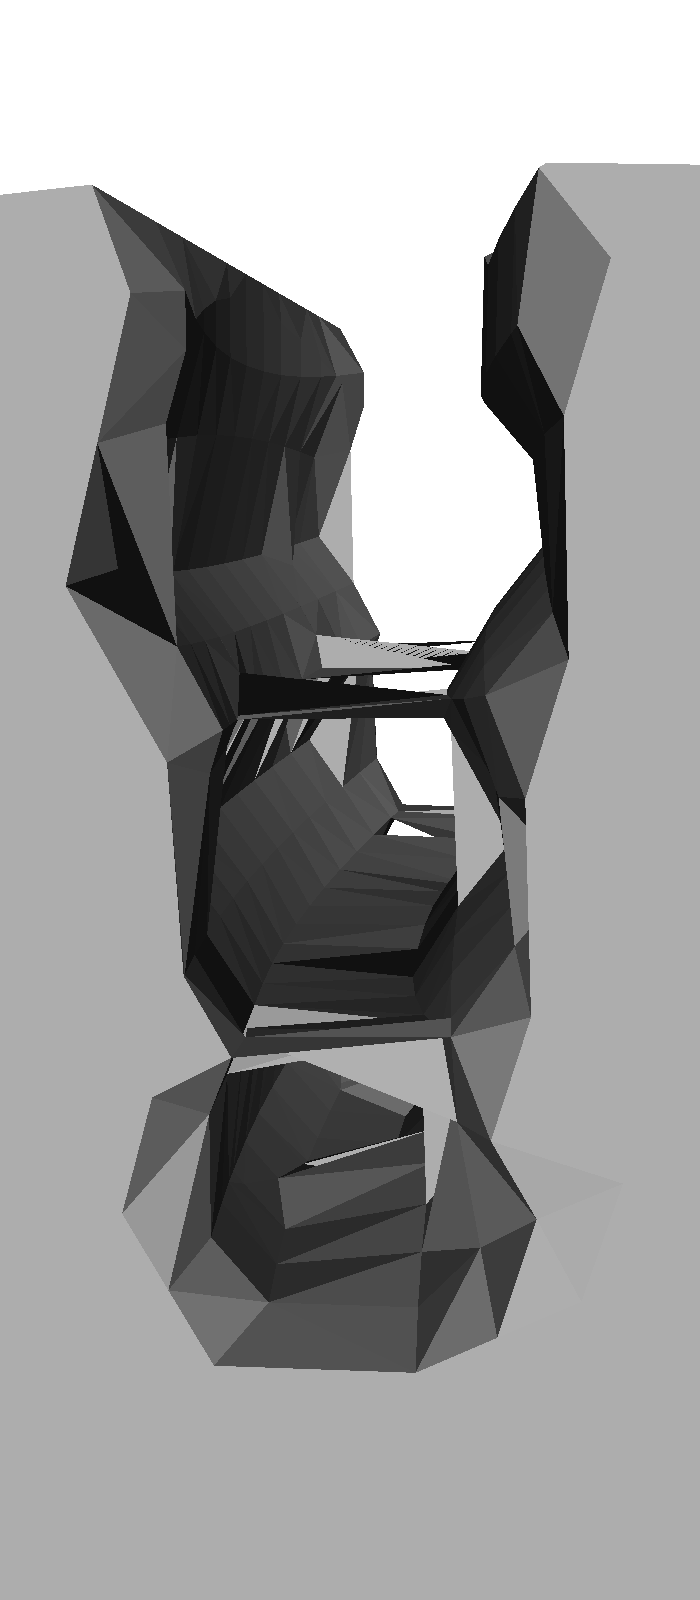
\includegraphics[width=\textwidth]{bpa_turbine_groove_100}
		\caption{100}
		\label{fig:bpa_turbine_groove_100}
	\end{subfigure}
	\begin{subfigure}[b]{0.24\textwidth}
		\centering
		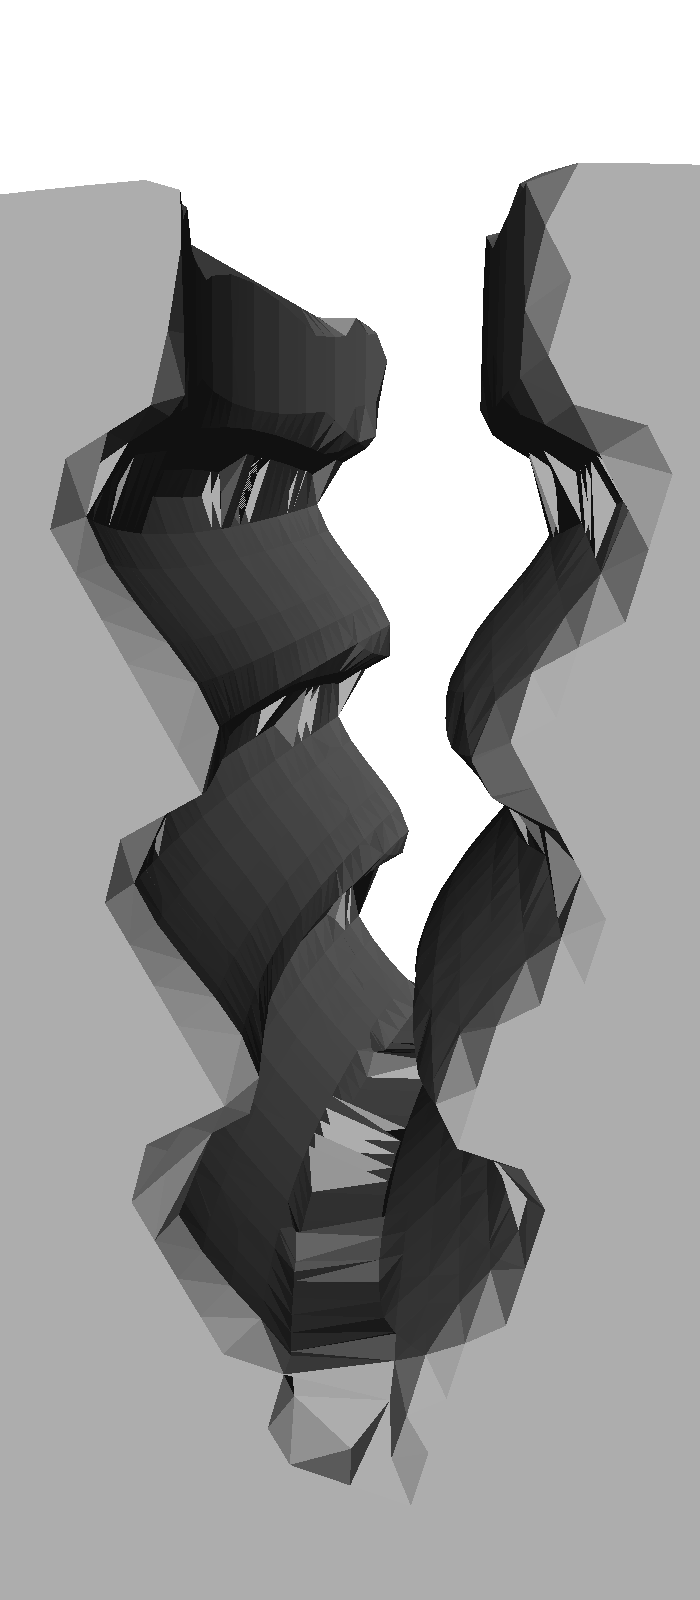
\includegraphics[width=\textwidth]{bpa_turbine_groove_200}
		\caption{200}
		\label{fig:bpa_turbine_groove_200}
	\end{subfigure}
	\begin{subfigure}[b]{0.24\textwidth}
		\centering
		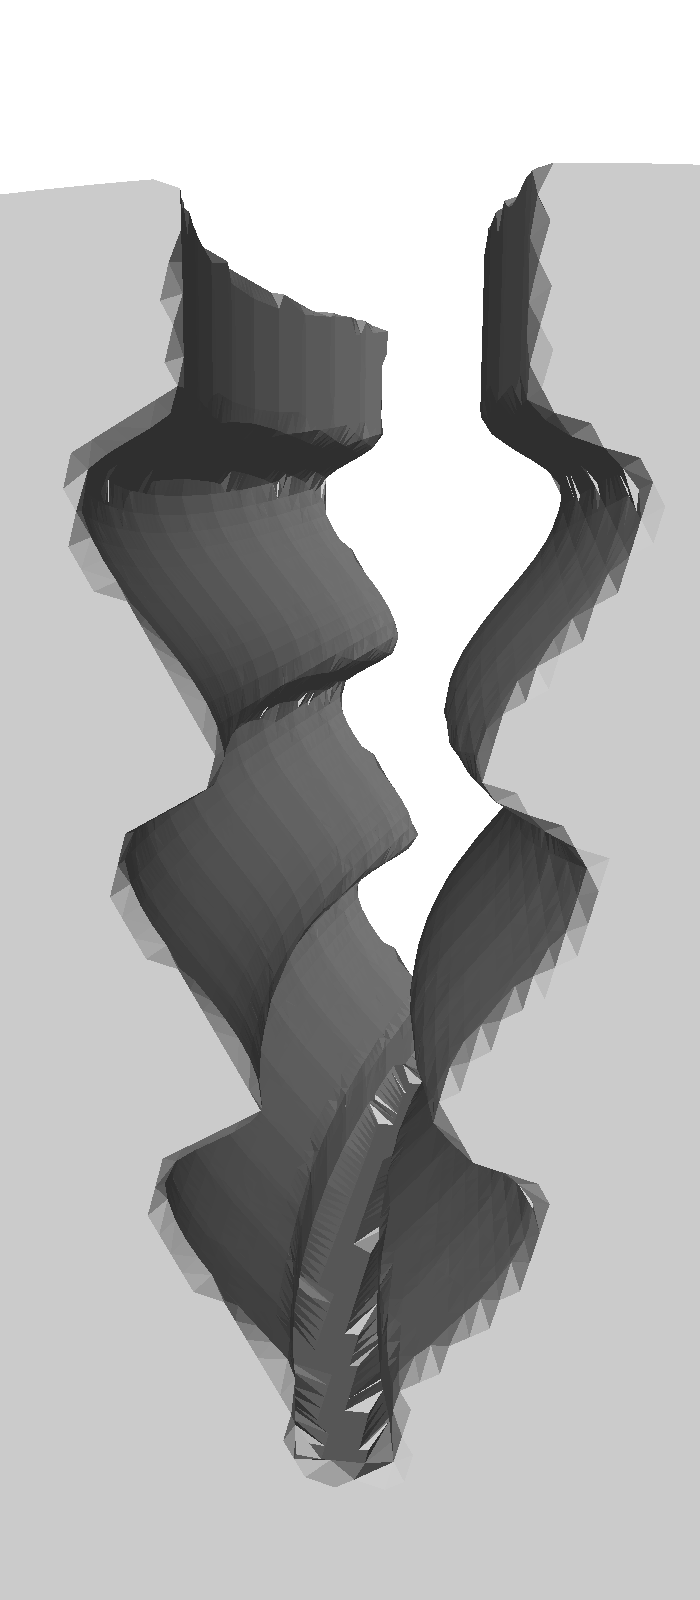
\includegraphics[width=\textwidth]{bpa_turbine_groove_400}
		\caption{400}
		\label{fig:bpa_turbine_groove_400}
	\end{subfigure}
	\caption[BPA \turbine grooves]{
		Detailed renderings with the same perspective of a groove of the \turbine scene.
		The meshes were created using the BPA reconstruction algorithm run on a point cloud with the resolutions 50, 100, 200 and 400.
	}
	\label{fig:bpa_grooves}
\end{figure}

Problematic cases for the BPA are shown in \cref{fig:bpa_issues}.

\begin{figure}
	\centering
	\begin{subfigure}[b]{0.49\textwidth}
		\centering
		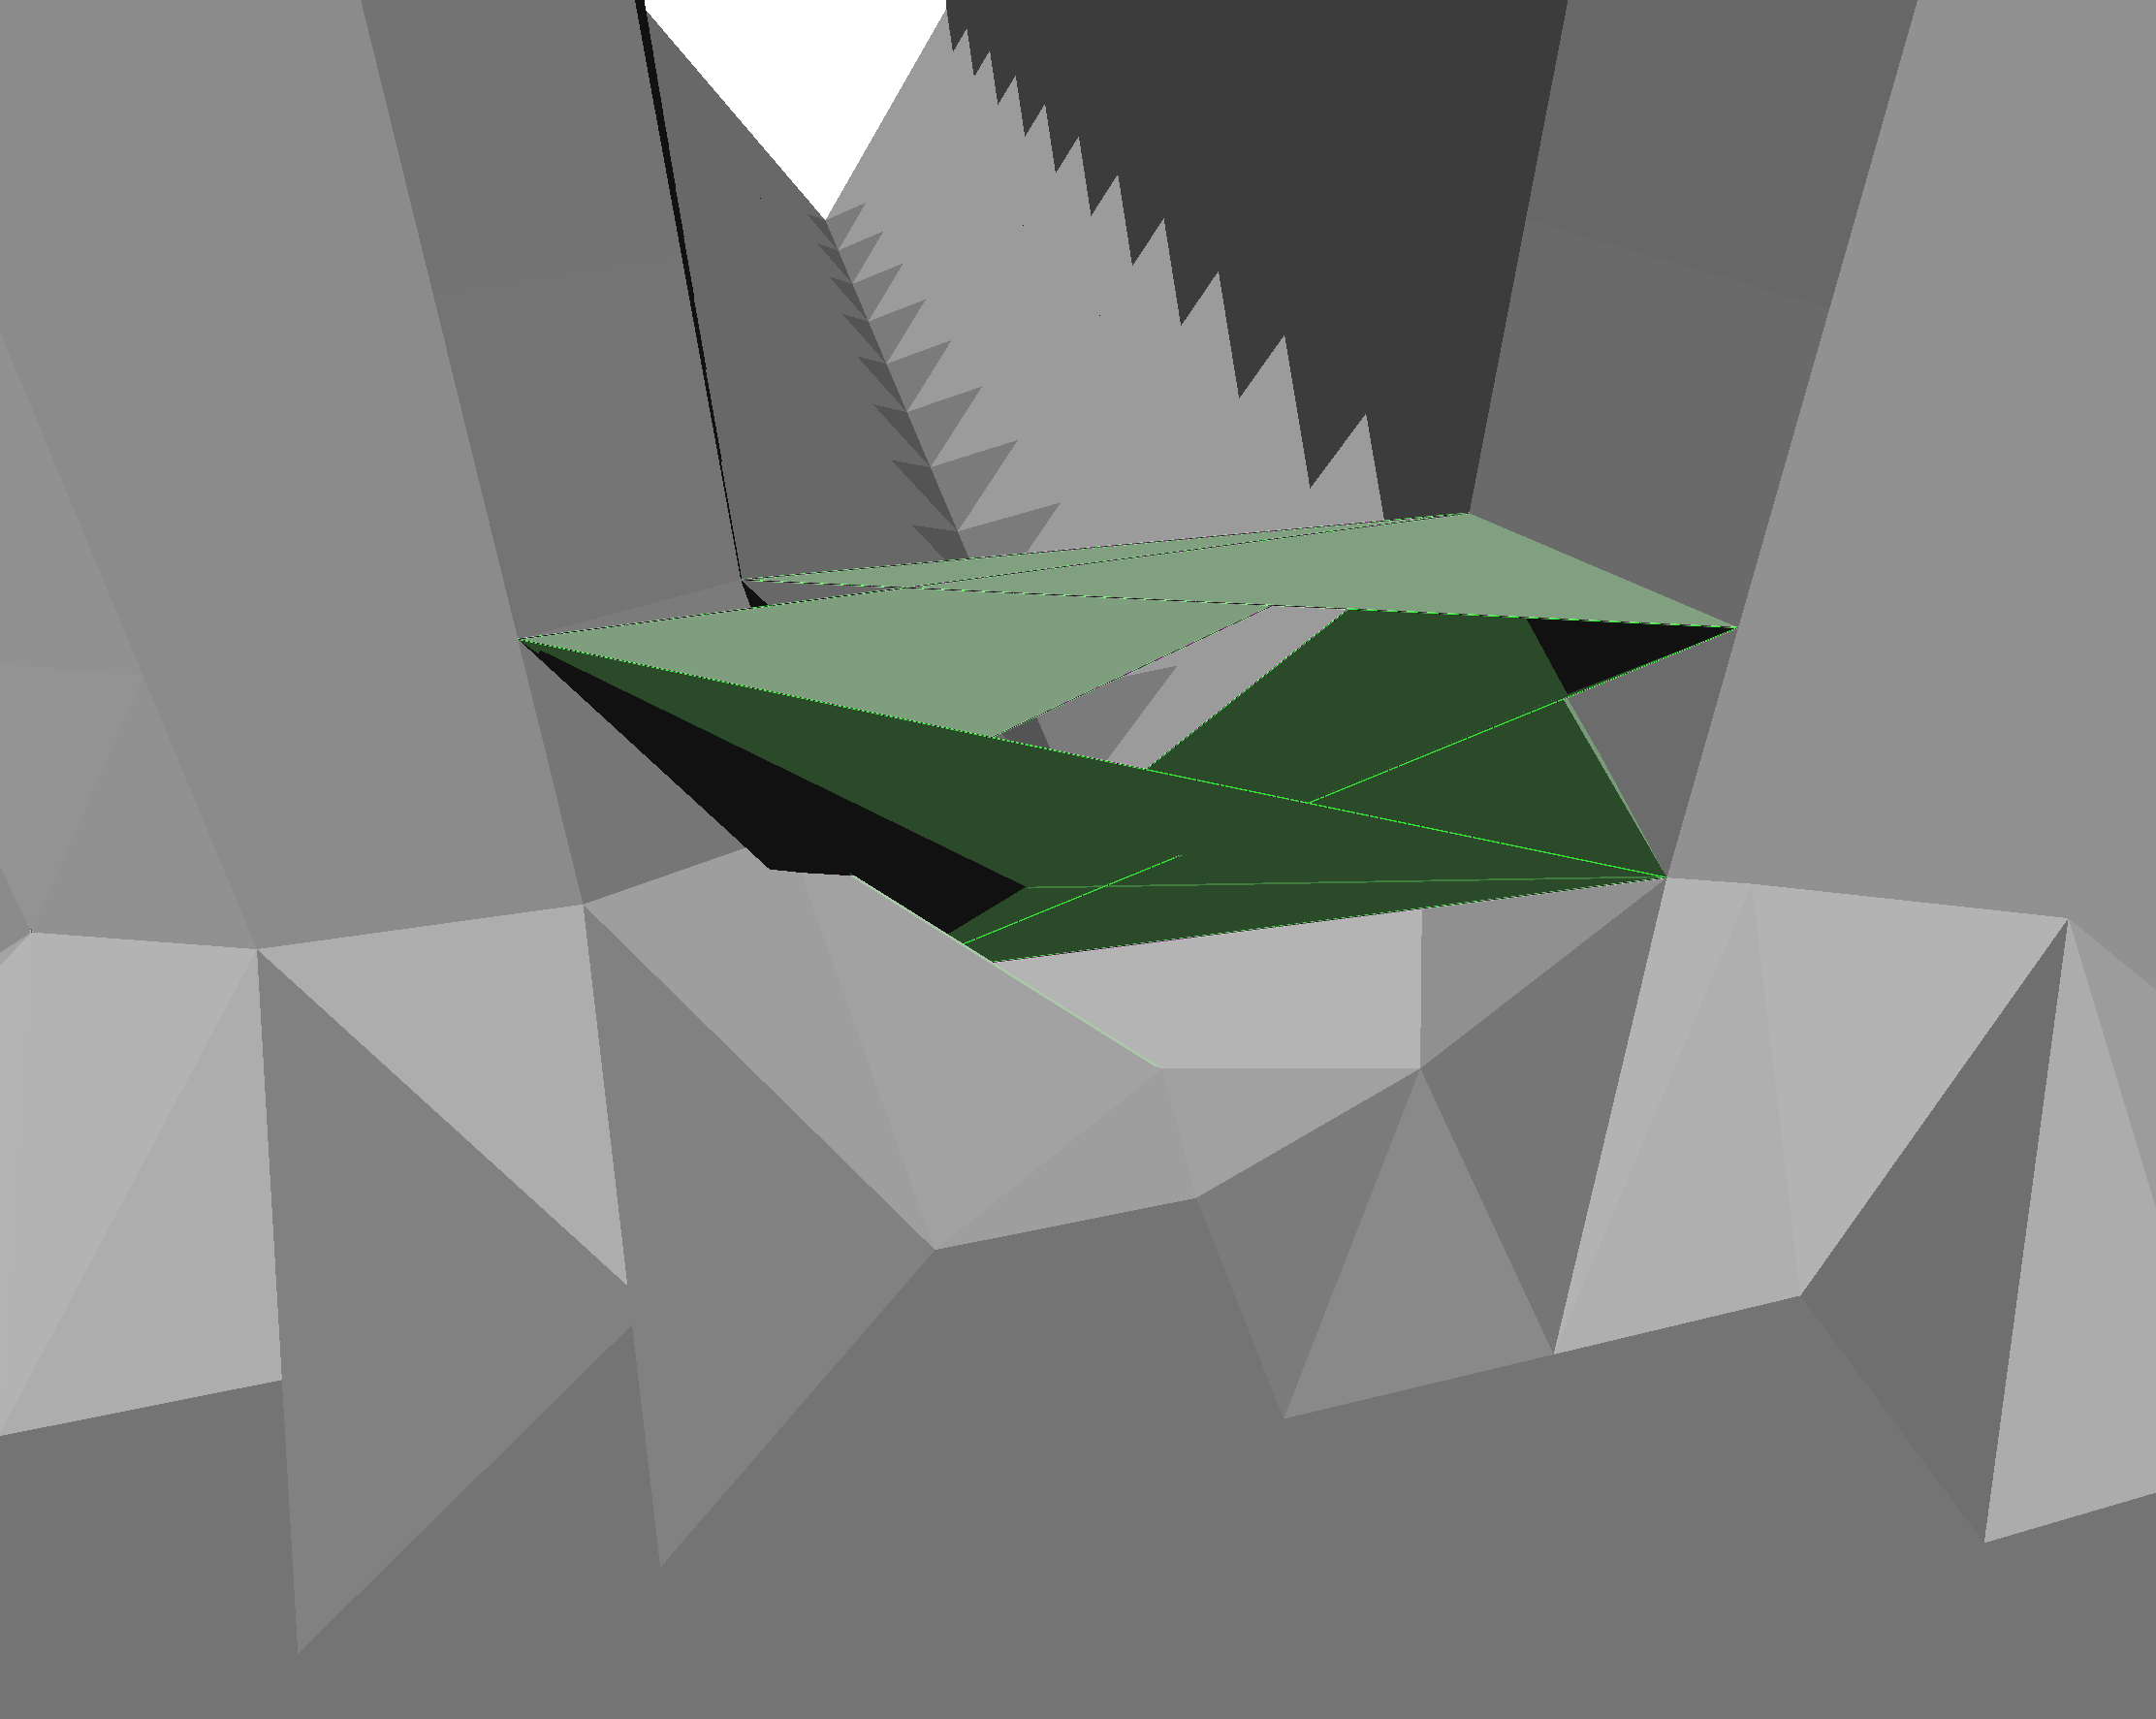
\includegraphics[width=\textwidth]{bpa_cylinder_head_non_manif}
		\caption{\cylinderhead 50}
		\label{fig:bpa_cylinder_head_non_manif}
	\end{subfigure}
	\begin{subfigure}[b]{0.49\textwidth}
		\centering
		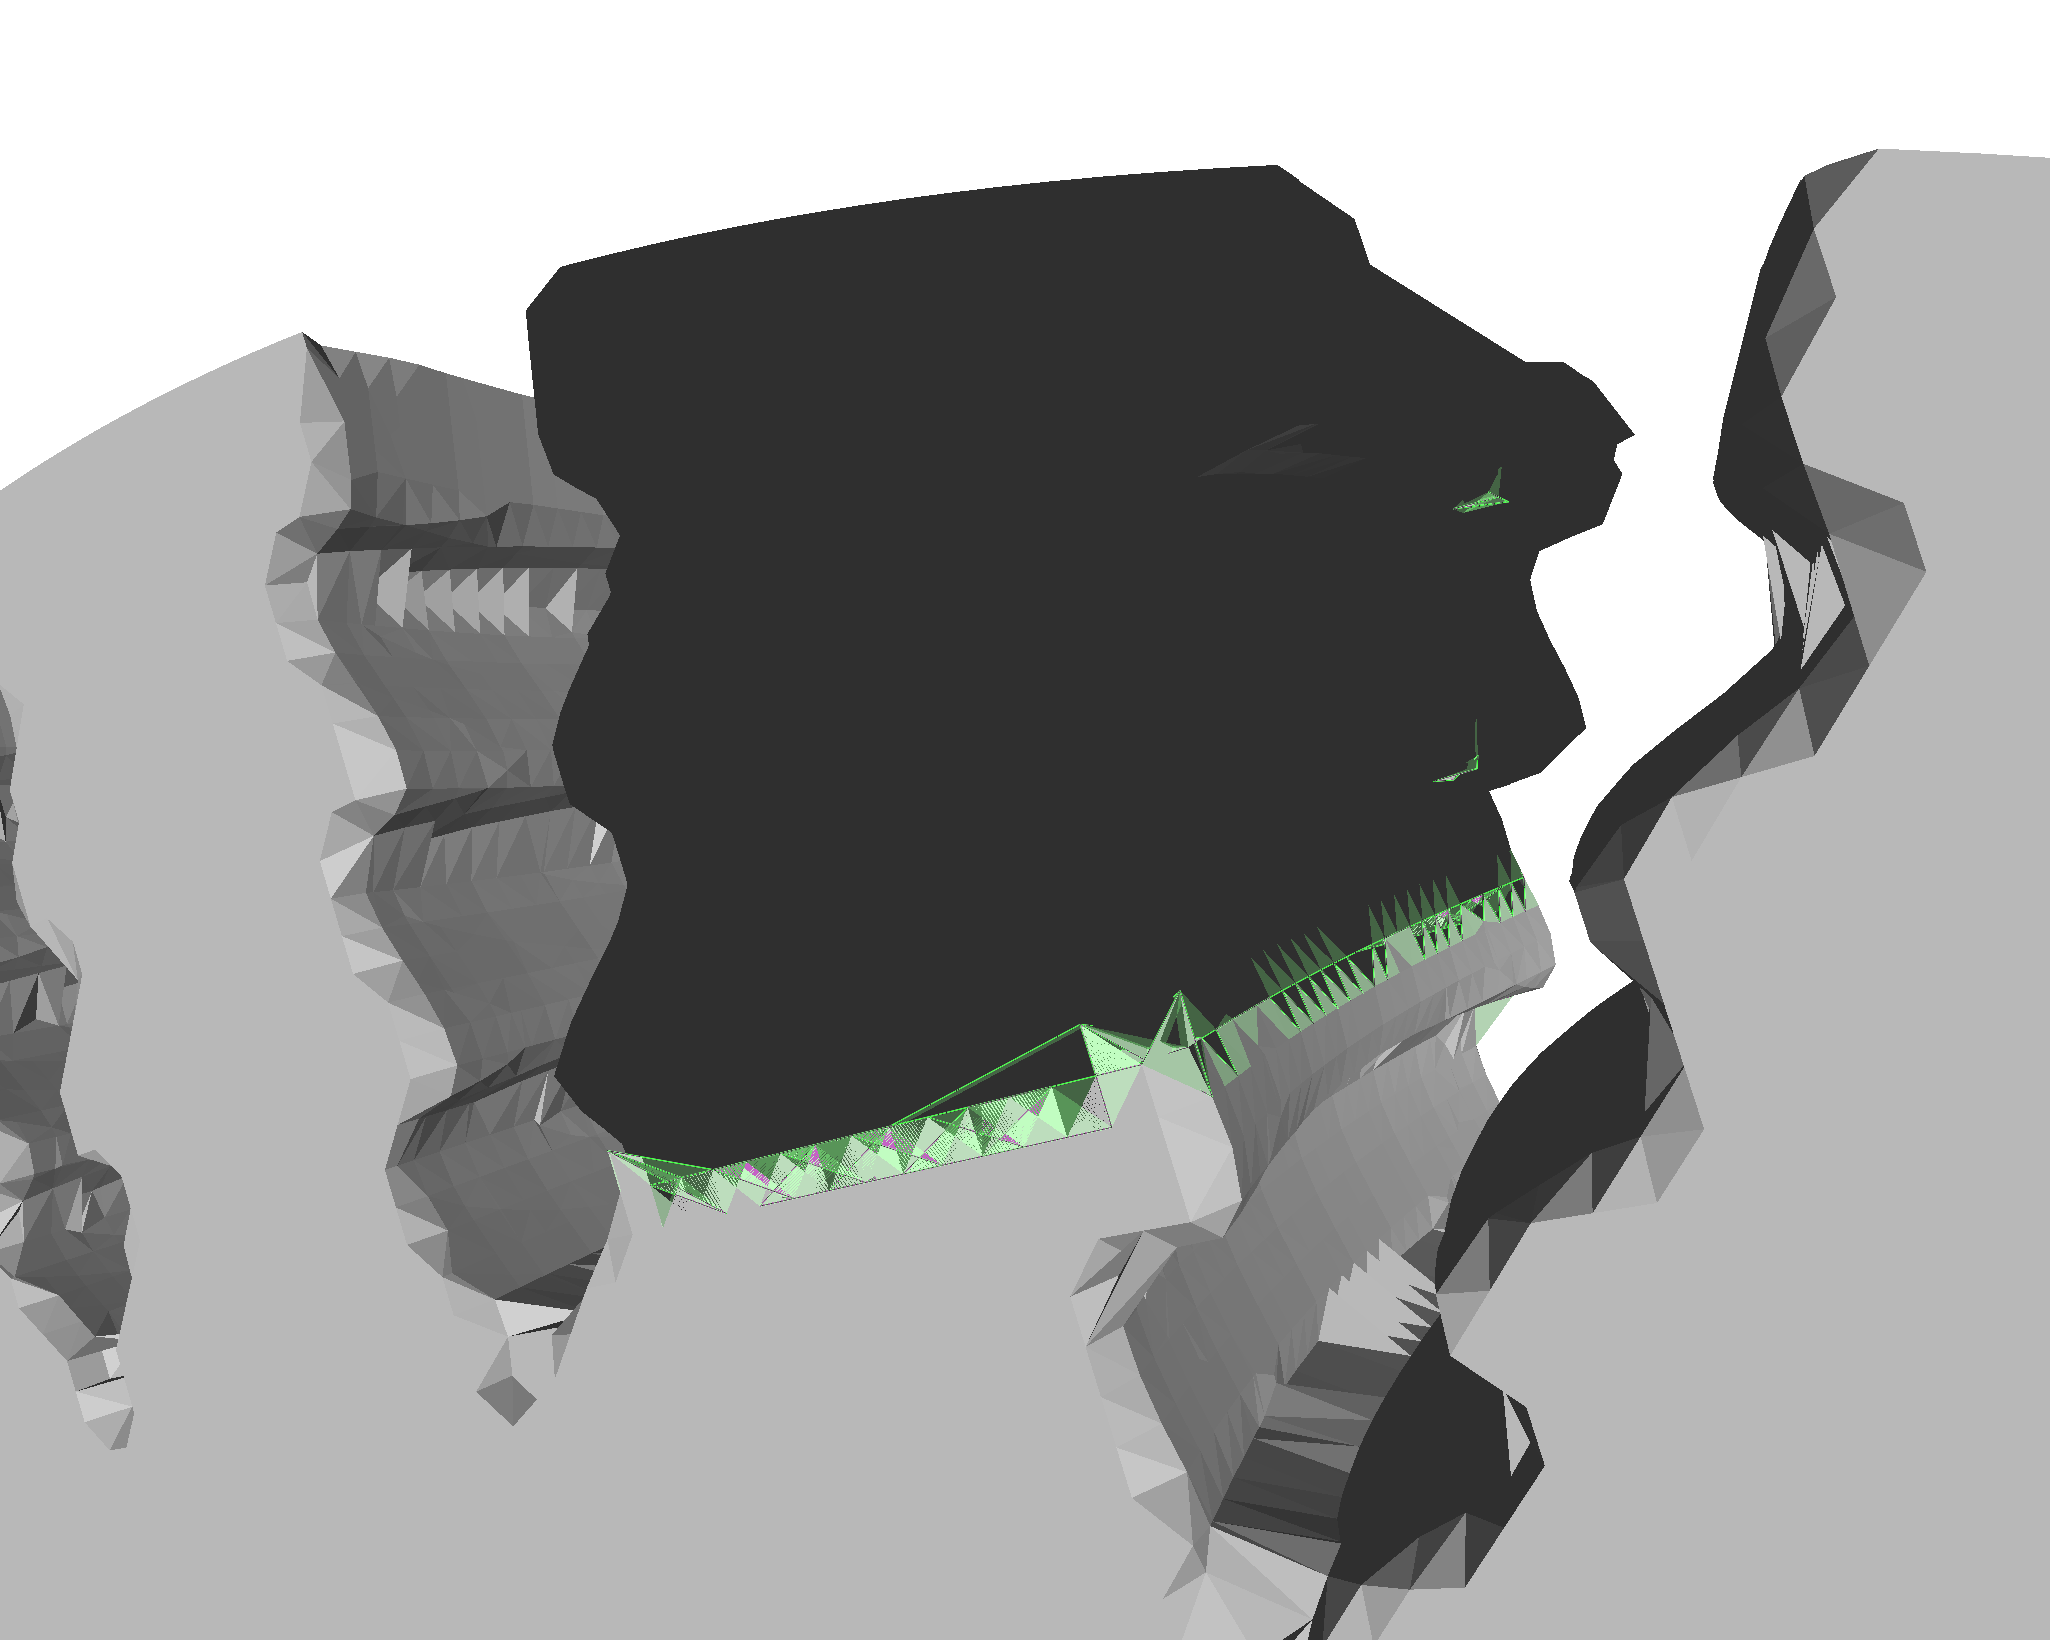
\includegraphics[width=\textwidth]{bpa_turbine_inside}
		\caption{\turbine 200}
		\label{fig:bpa_turbine_inside}
	\end{subfigure}
	\caption[BPA artifacts]{
		Error in the \cylinderhead and \turbine scene after BPA reconstruction.
		Boundary edges are marked in green.
	}
	\label{fig:bpa_issues}
\end{figure}

The created boundary edges of the BPA are listed in \cref{tbl:bpa_boundary edges}.

\begin{table}
	\centering
	\begin{tabular}{l|r|r|r|r}
		resolution    &  50 &  100 &  200 &  400 \\
		\midrule
		\cubes        &   0 &    0 &    0 &    0 \\
		\cylindersd   &   0 &    0 &    0 &    0 \\
		\cylinders    &   0 &    0 &    0 &    0 \\
		\cylinderhead & 110 &    0 &    0 &    0 \\
		\impeller     &   0 &    0 &    0 &    0 \\
		\impellerhalf &   0 &    0 &    0 &    0 \\
		\turbine      &   0 & 3055 & 1721 & 3293 \\
	\end{tabular}
	\caption[BPA boundary edges]{
		Created boundary edges by the BPA surface extraction.
	}
	\label{tbl:bpa_boundary edges}
\end{table}

\Cref{fig:poisson_results} shows renderings of the \cylinderhead and \impeller scene after applying the Poisson surface reconstruction filter available in MeshLab.

\begin{figure}
	\centering
	\begin{subfigure}[b]{0.49\textwidth}
		\centering
		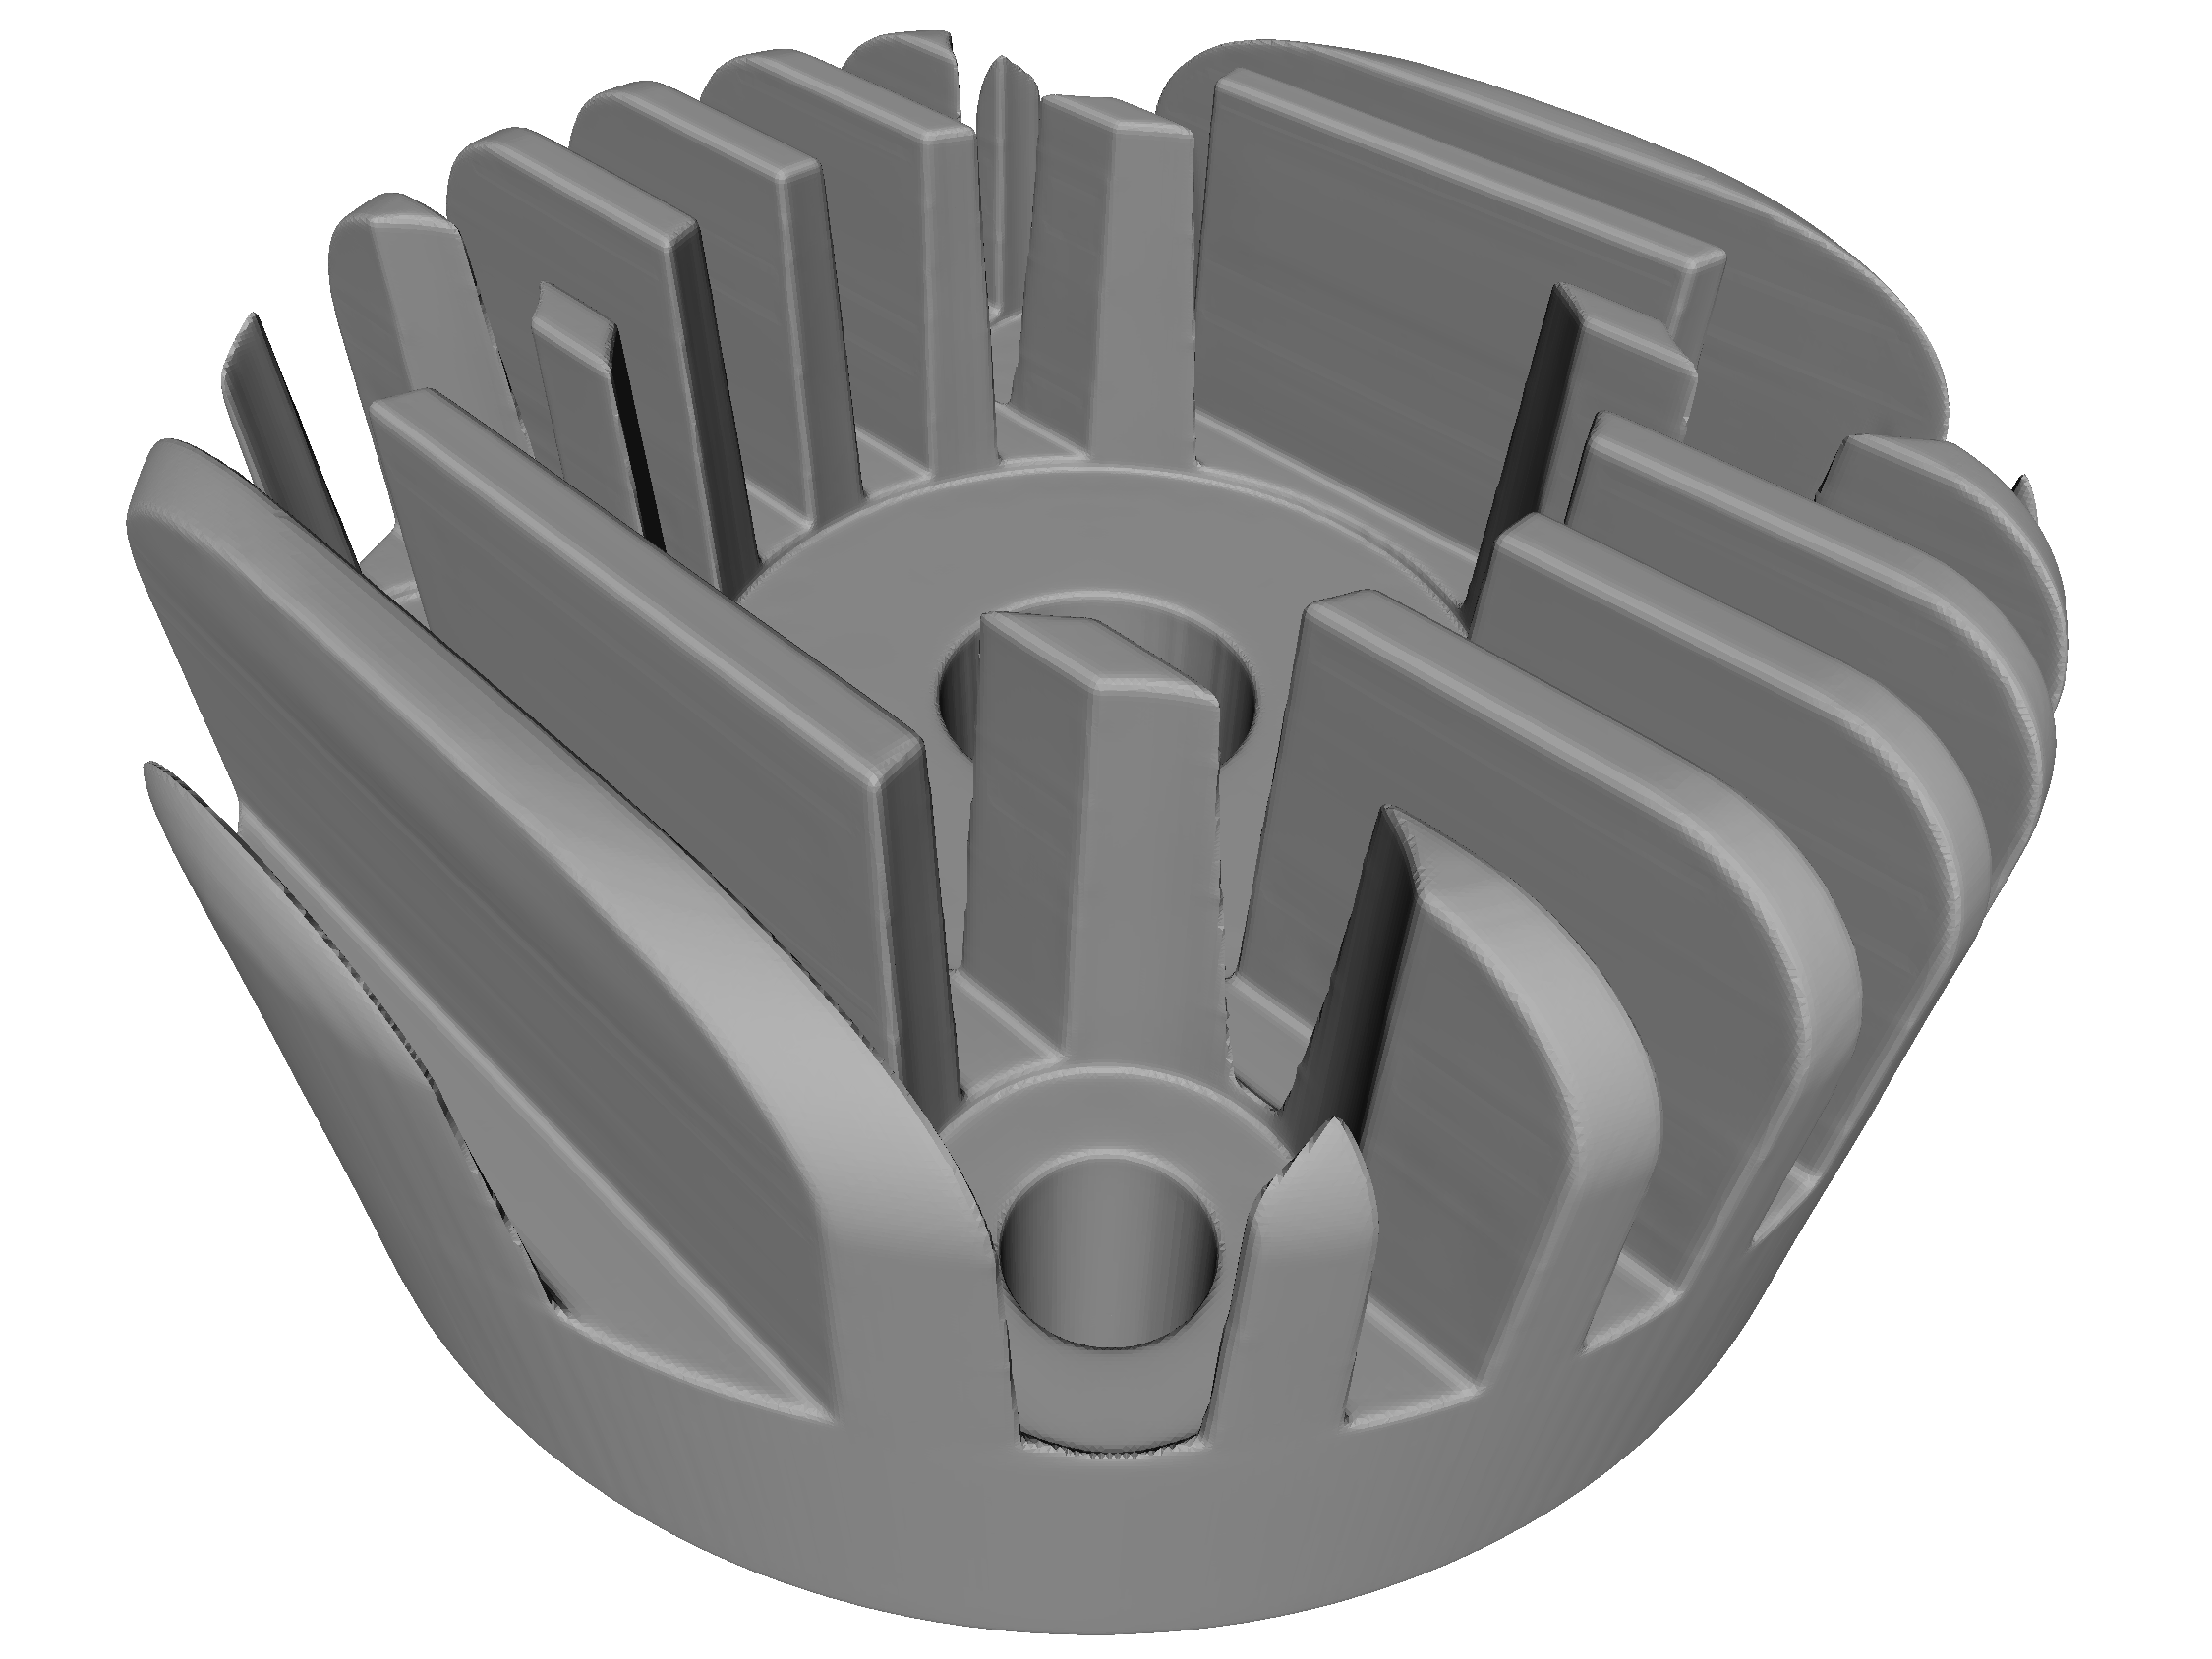
\includegraphics[width=\textwidth]{poi_cylinder_head}
		\caption{\cylinderhead}
		\label{fig:poi_cylinder_head}
	\end{subfigure}
	\begin{subfigure}[b]{0.49\textwidth}
		\centering
		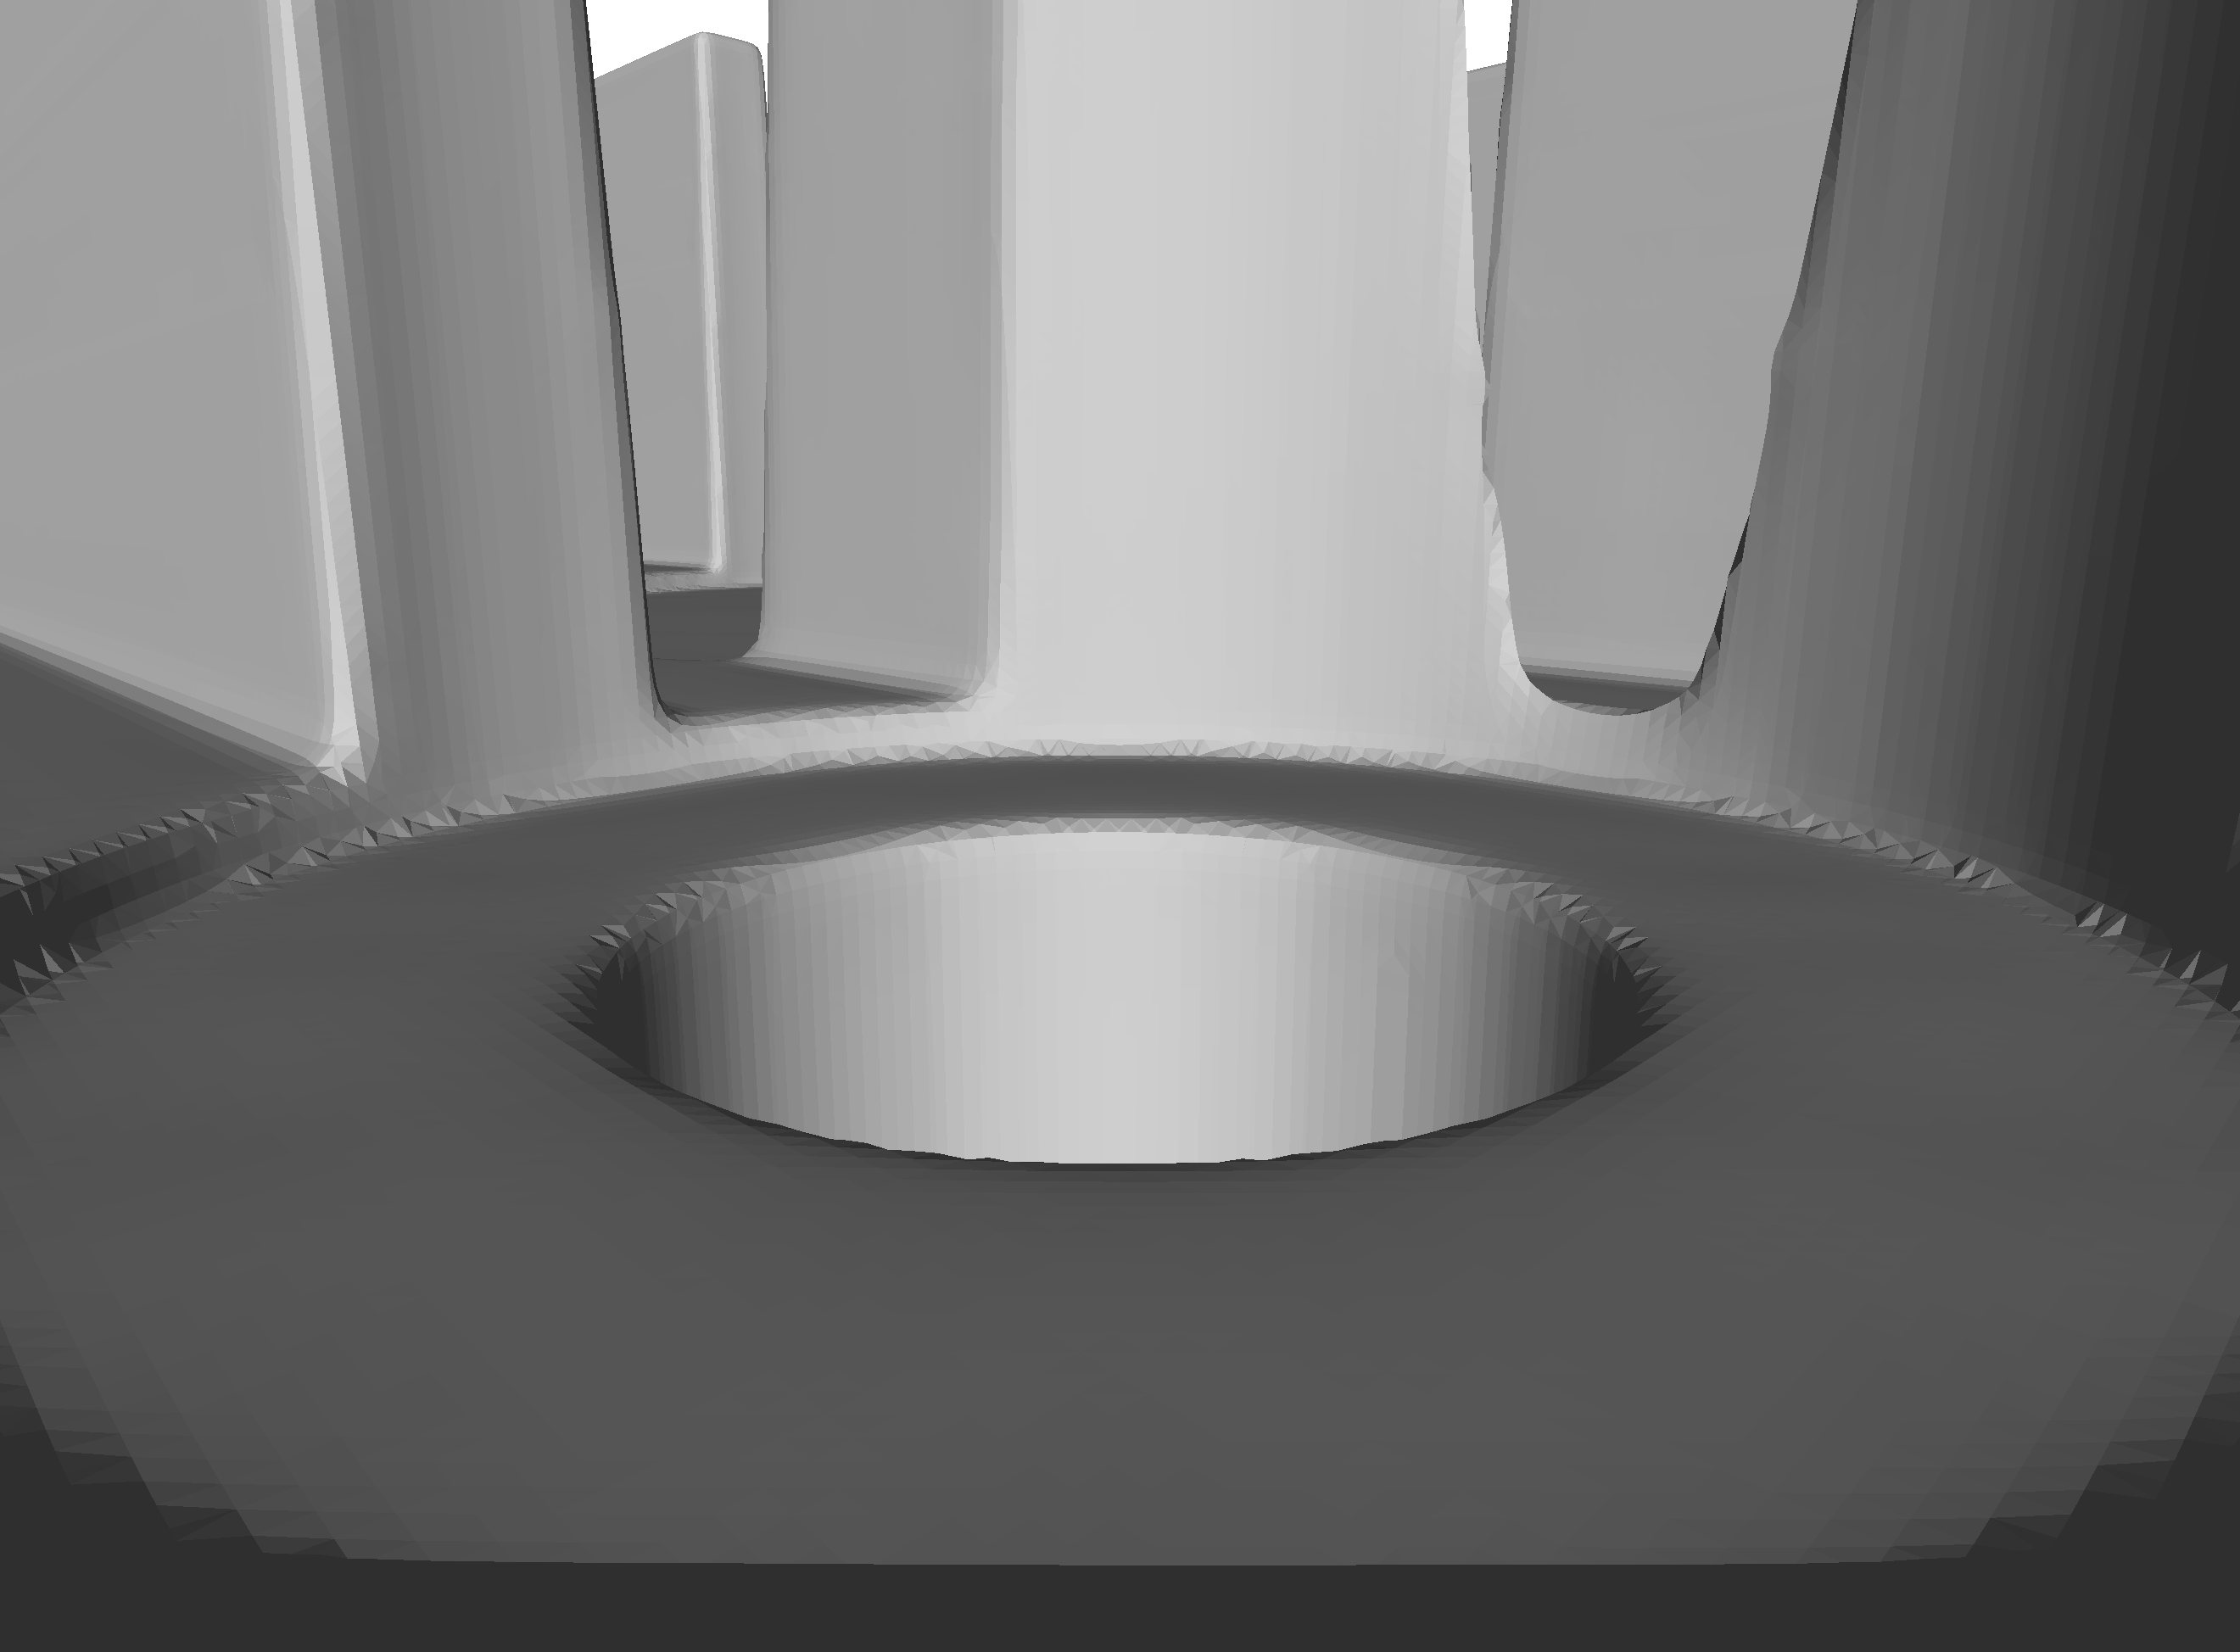
\includegraphics[width=\textwidth]{poi_cylinder_head_detail}
		\caption{\cylinderhead details}
		\label{fig:poi_cylinder_head_detail}
	\end{subfigure}
	\begin{subfigure}[b]{0.49\textwidth}
		\centering
		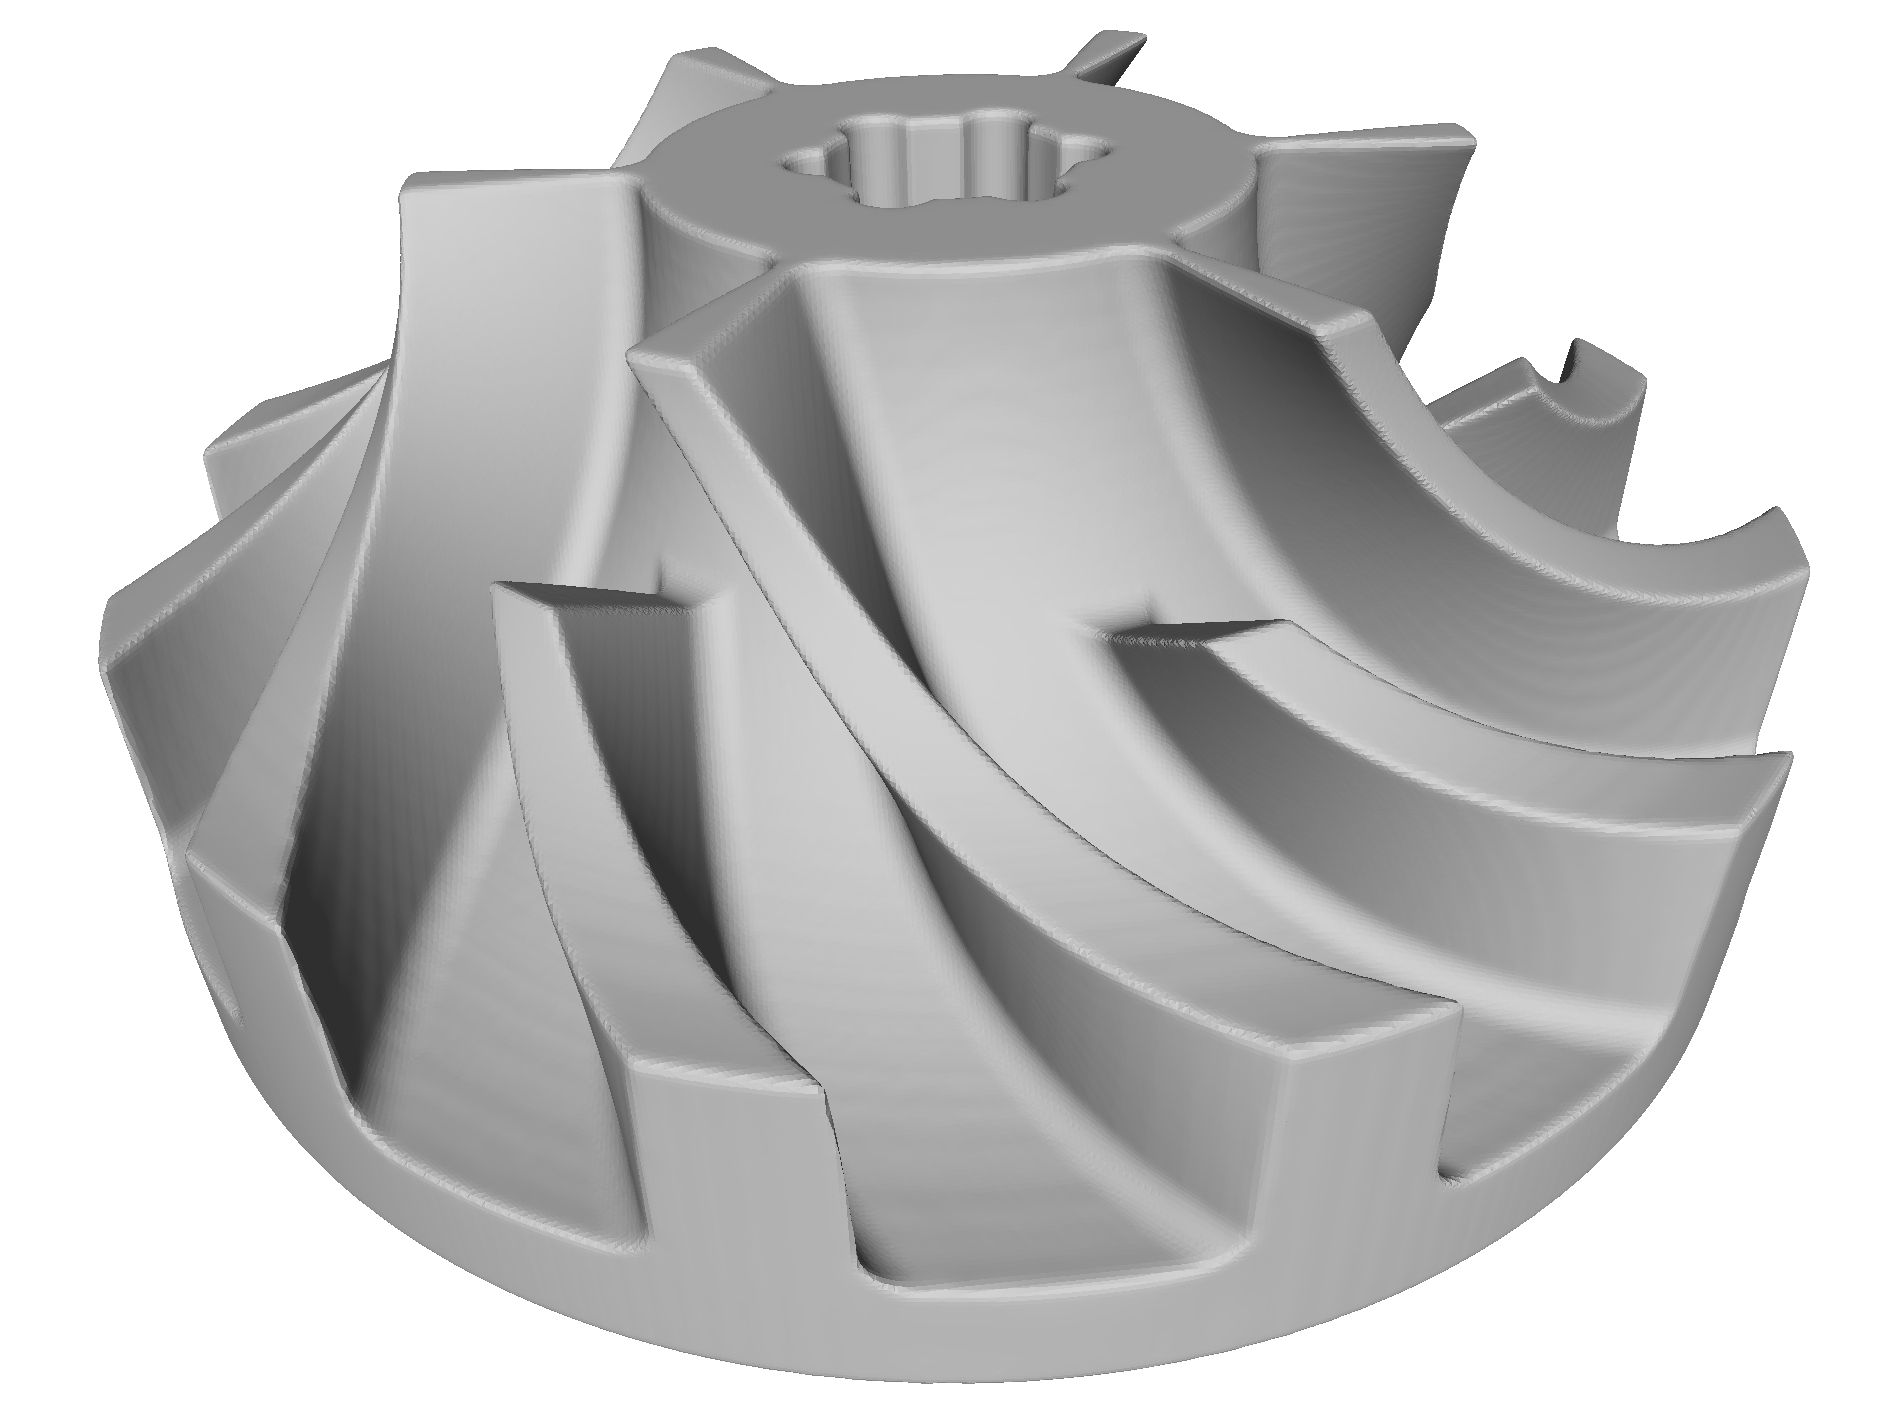
\includegraphics[width=\textwidth]{poi_hq_impeller}
		\caption{\impeller}
		\label{fig:poi_hq_impeller}
	\end{subfigure}
	\begin{subfigure}[b]{0.49\textwidth}
		\centering
		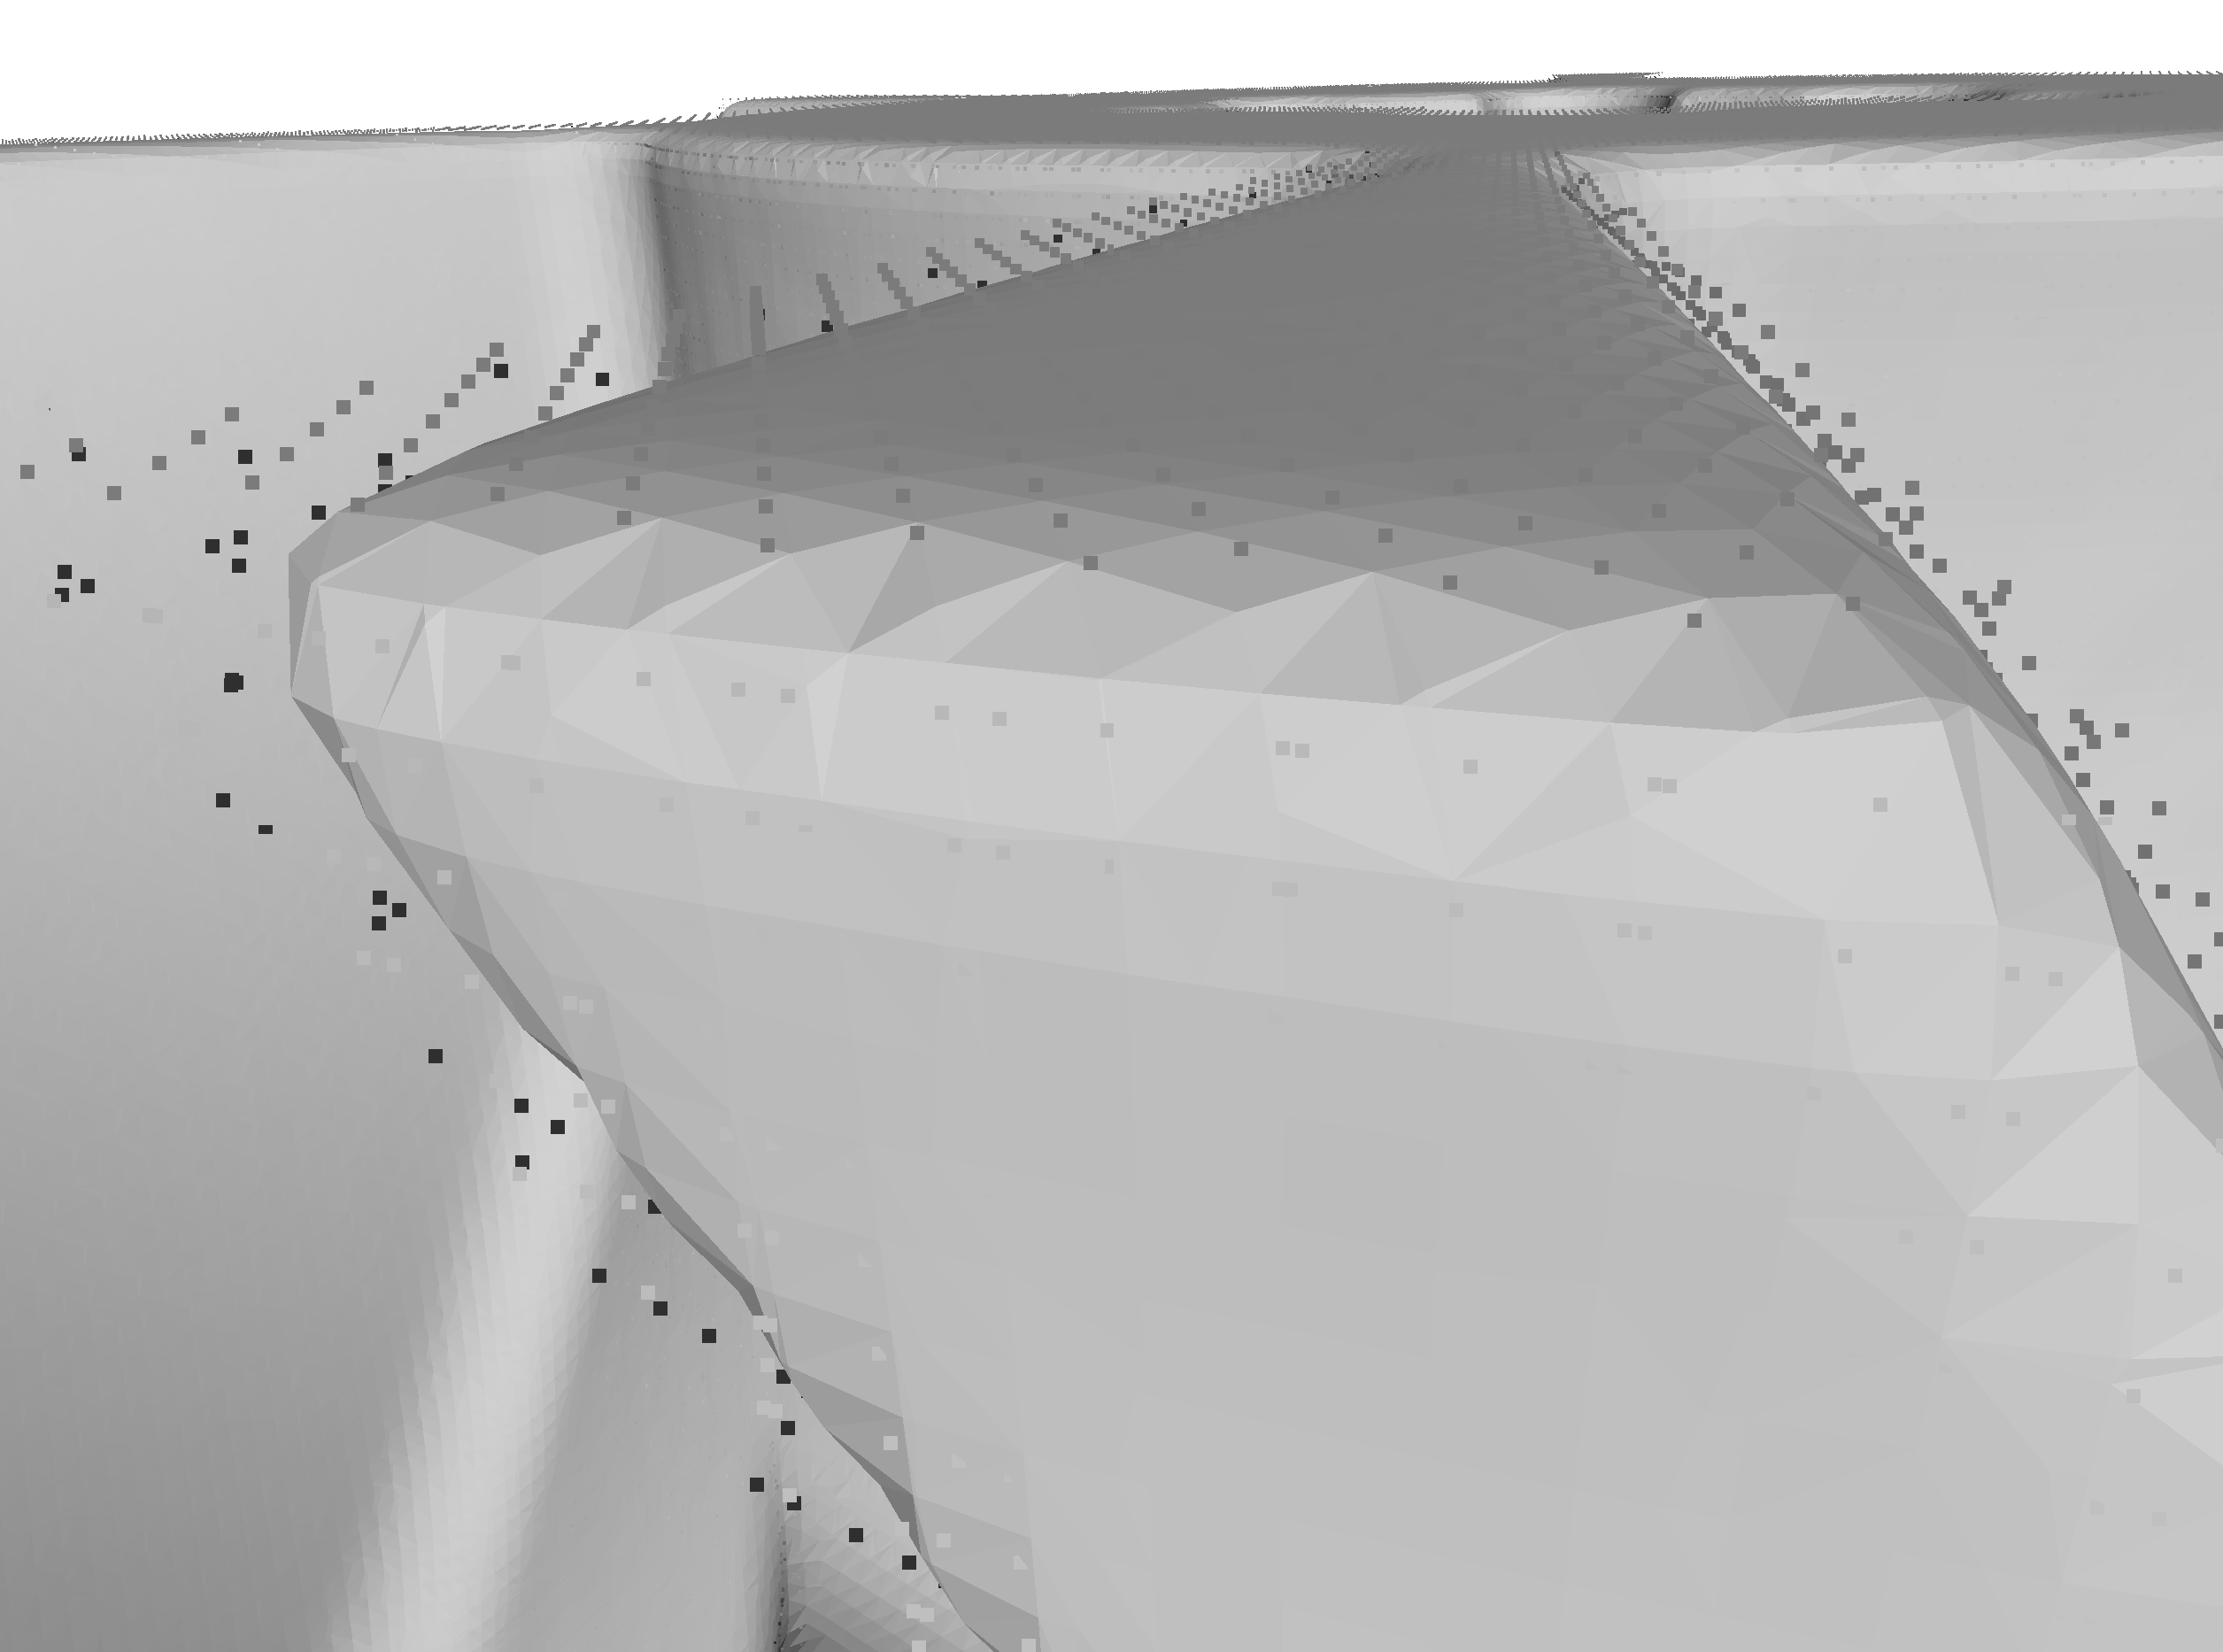
\includegraphics[width=\textwidth]{poi_hq_impeller_points}
		\caption{\impeller edges}
		\label{fig:poi_hq_impeller_points}
	\end{subfigure}
	\caption[Poisson result renderings]{
		Renderings of the \cylinderhead and \impeller scenes of reconstructions using the Poisson surface reconstruction filter from MeshLab.
		The point cloud was created with a resolution of 400.
		The Poisson filter was parameterized with an octree depth of ten, solver divide at eight, one sample per node and a surface offsetting of one, \cf corresponding dialog in MeshLab.
	}
	\label{fig:poisson_results}
\end{figure}

\Cref{fig:poi_grooves} shows a groove of the \turbine reconstructed from point clouds with various resolutions.

\begin{figure}
	\begin{subfigure}[b]{0.24\textwidth}
		\centering
		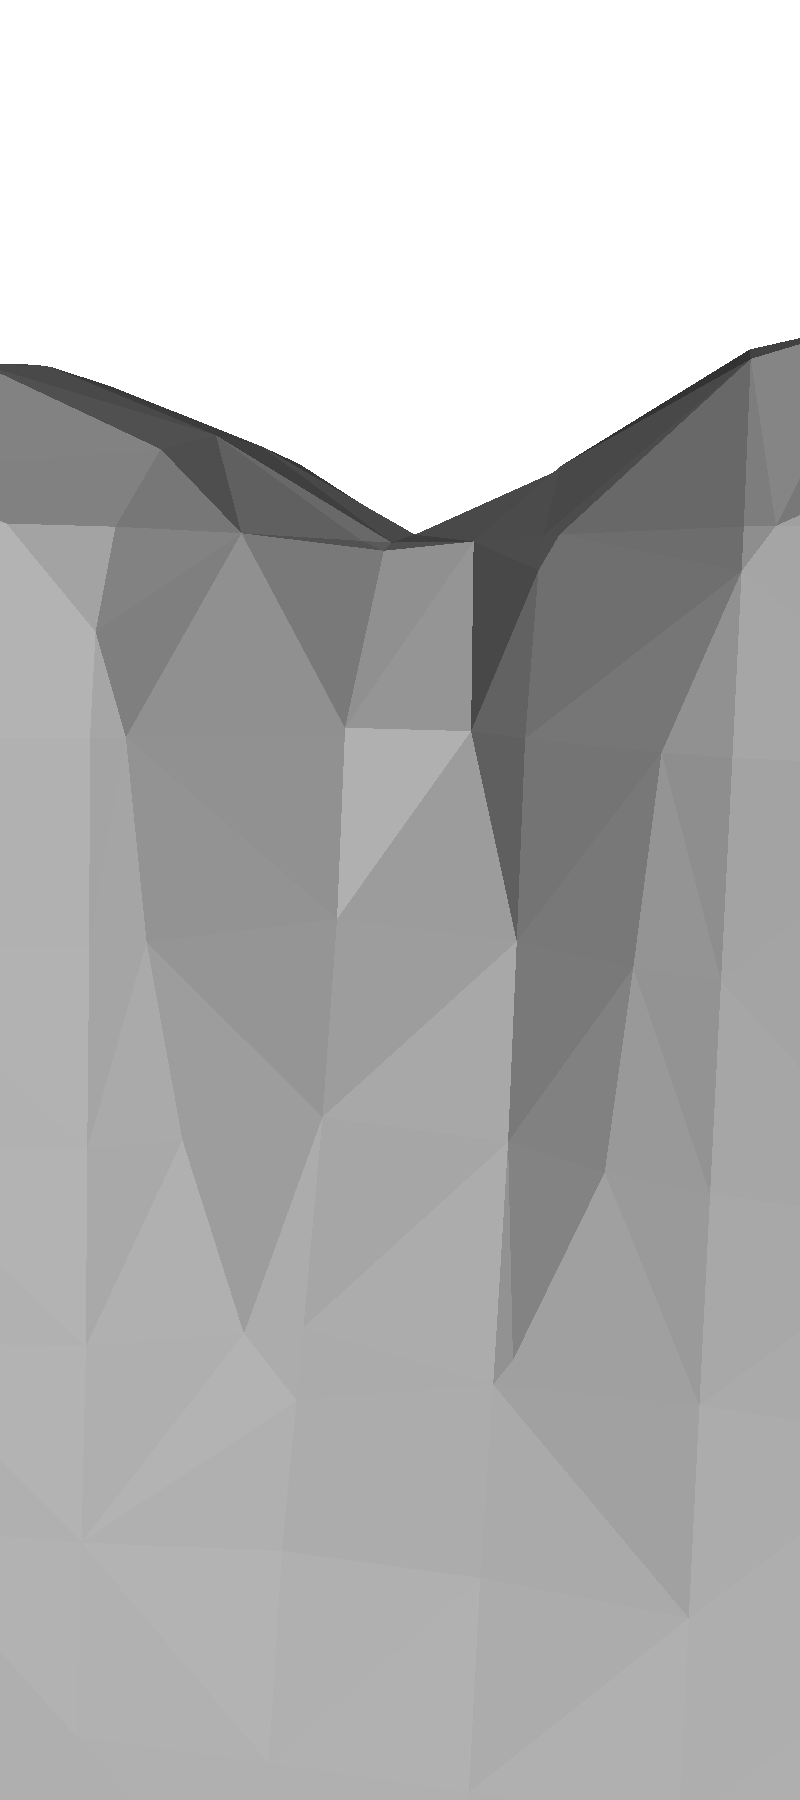
\includegraphics[width=\textwidth]{poi_turbine_groove_50}
		\caption{50}
		\label{fig:poi_turbine_groove_50}
	\end{subfigure}
	\begin{subfigure}[b]{0.24\textwidth}
		\centering
		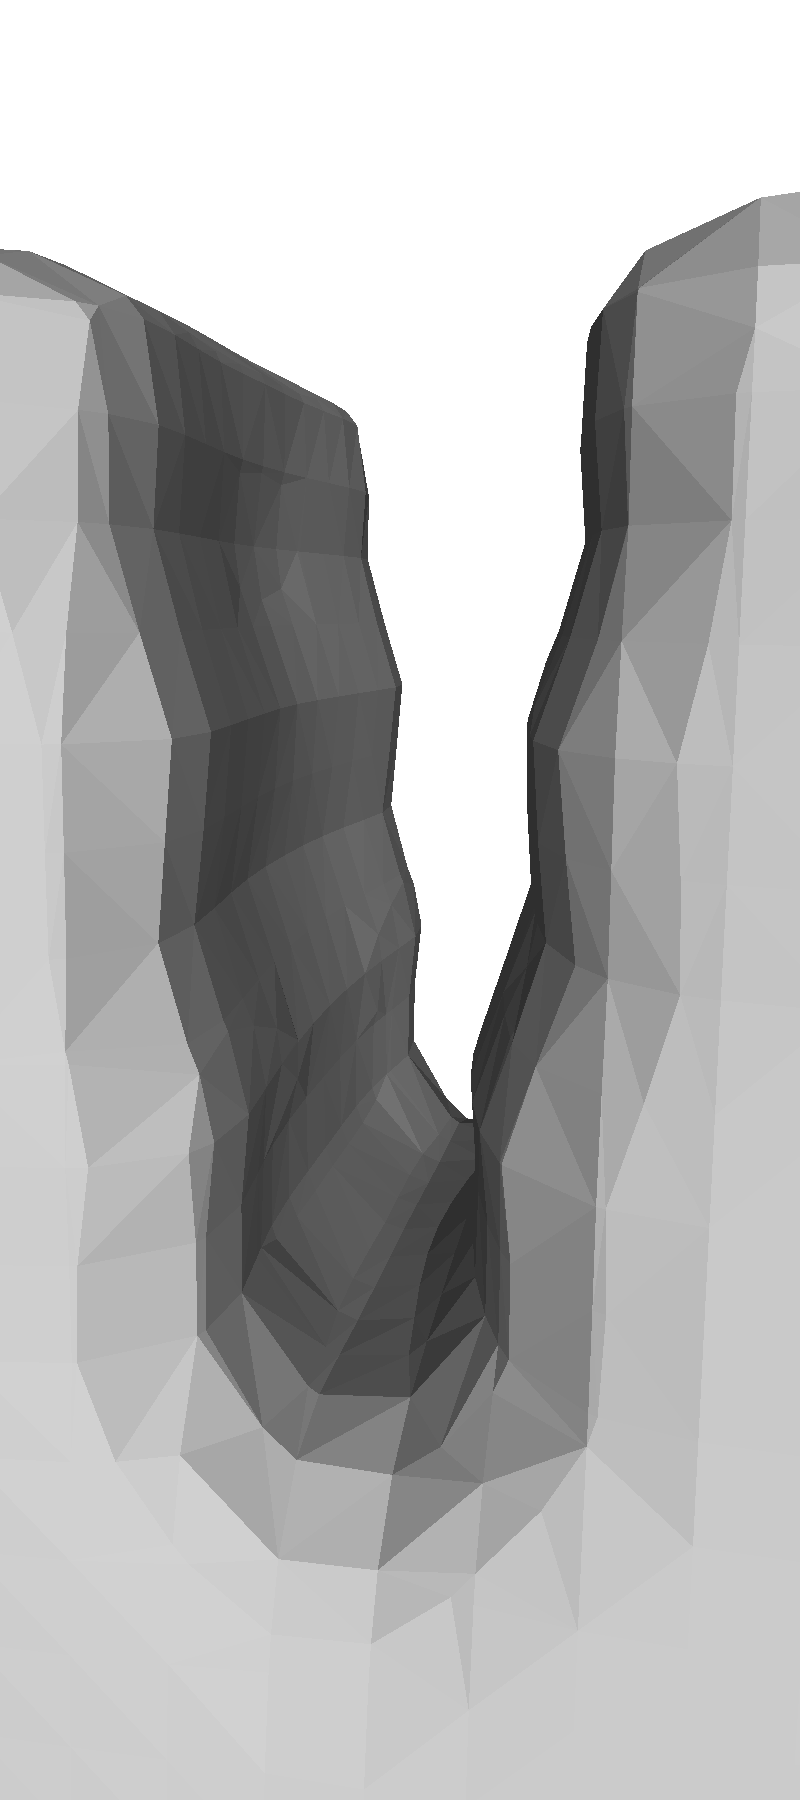
\includegraphics[width=\textwidth]{poi_turbine_groove_100}
		\caption{100}
		\label{fig:poi_turbine_groove_100}
	\end{subfigure}
	\begin{subfigure}[b]{0.24\textwidth}
		\centering
		\includegraphics[width=\textwidth]{poi_turbine_groove_200}
		\caption{200}
		\label{fig:poi_turbine_groove_200}
	\end{subfigure}
	\begin{subfigure}[b]{0.24\textwidth}
		\centering
		\includegraphics[width=\textwidth]{poi_turbine_groove_400}
		\caption{400}
		\label{fig:poi_turbine_groove_400}
	\end{subfigure}
	\caption[Poisson \turbine grooves]{
		Detailed renderings with the same perspective of a groove of the \turbine scene.
		The meshes were created using the Poisson surface reconstruction filter of MeshLab.
	}
	\label{fig:poi_grooves}
\end{figure}

\endgroup
